\documentclass[../../book-main.tex]{subfiles}
\usepackage[UTF8]{ctex}
\graphicspath{{\subfix{../..}}}

\begin{document}

\chapter{通过展开优化实现深度表示}
\label{ch:representation}
\label{ch:unrolling}

\begin{quote}
\hfill    ``{\em 我所不能创造的,我就不理解}。''

$~$ \hfill --- 理查德·费曼
\end{quote}
\vspace{5mm}

% {\yaodong{第一章的笔记:``正如我们将在本书中看到的,答案直到最近才被发现:非线性问题可以通过渐进的线性化和变换来有效处理,这可以通过深度神经网络实现(见第 \ref{ch:representation} 章)。此外,我们将在本书中尝试展示,如何将上面列出的所有这些机制自然地整合到一个完整的学习系统中,该系统展现出自主智能系统的特征(见第 \ref{ch:autoencoding} 章和第 \ref{ch:closed-loop} 章)。''}}

% \yima{从前一章的过渡:除了通过最小化编码率来识别低维分布外,学习还有一个额外的目标:使表示更具信息量或结构化。因此,我们需要最大化信息增益,其中最小化低维分布的熵是其中的一部分。}

% \yima{设定背景:我们使用高斯(子空间)或高斯混合(子空间)作为原型分布,用于(近似)建模任何感兴趣的分布。}

在前面的章节中,我们已经展示了如何在多维空间中识别低维结构,\textit{主要关注线性结构}。
例如,当观测数据 $\bm{x}$ 服从统计模型 $\bm{x} = \bm{U}\bm{z} + \bm{\varepsilon}$ 时,我们介绍了主成分分析(PCA)来学习线性去噪器 $\hat{\bm{U}}^{\top}$。
在这种情况下,学习到的表示是线性变换后的输入数据 $\hat{\bm{U}}^{\top}\bm{x}$。
在线性模型假设下,人们可以用高效的优化算法和强大的理论保证来学习低维线性结构。
此外,线性模型假设涵盖了广泛的应用和问题,包括人脸识别、磁共振图像恢复以及结构纹理恢复~\cite{Wright-Ma-2022}。

另一方面,在处理现实世界的应用时,线性模型可能会受到限制,特别是当输入数据 $\bm{x}$ 很复杂时,例如语音和自然语言、图像和视频以及机器人运动。这类数据的低维分布通常是非线性的。
如何处理非线性问题在控制论、信号处理和模式识别等不同学科中有着悠久的历史。人们已经付出了相当大的努力,试图将线性模型的方法和解决方案扩展到处理非线性问题,包括早期将 PCA 扩展到非线性 PCA 的努力(我们将在第 \ref{ch:autoencoding} 章中更详细地研究)。在大多数情况下,这些方法是基于关于数据分布的某些假设而设计的,并针对特定问题量身定制。

最近,深度神经网络在各种数据和应用中取得了显著的成功。一个神经网络
\begin{equation}
  f(\cdot, \bm \theta) \colon \x
  \xrightarrow{\hspace{1mm} f^0 \hspace{1mm}} \z^0 \rightarrow \cdots
  \rightarrow \z^\ell \xrightarrow{\hspace{1mm} f^\ell \hspace{1mm}}
  \z^{\ell+1} \rightarrow  \cdots \to \z^L = \z.
\end{equation}
可以为下游应用学习有效的特征/表示。例如,一个训练好的深度神经网络 $f(\cdot, \bm \theta)$ 可以应用于将图像映射到表示向量,即 $\bm{z}_i = f(\bm{x}_i,\bm \theta)$,而线性分类器可以在这些表示 $\{\bm{z}_i\}$ 的基础上进行学习。一个显著的突破是 AlexNet~\cite{krizhevsky2012imagenet},这是一个用超过一百万张自然图像训练的深度卷积神经网络,其性能超过了所有以前基于手工制作特征的方法。AlexNet 与以前方法的一个关键区别是\textit{从海量数据中学习非线性变换的参数},并通过反向传播(BP)\cite{Back-Prop} 进行训练,详见附录 \ref{app:optimization} 的 \ref{app:BP-section} 节。


%\subsection{关于黑盒深度网络的谜团}
% 在不打断流程的情况下,提出关于通过深度神经网络进行表示学习的谜团。如何理解所有经验设计的深度神经网络的作用,这些网络在很大程度上是黑盒。

随后的流行做法是用其他经验设计的人工深度神经网络来建模映射 $f$,并通过反向传播(BP)从随机初始化中学习参数 $\bm \theta$。从 AlexNet \cite{krizhevsky2012imagenet} 开始,现代深度网络的架构不断被经验性地修正和改进。诸如 VGG \cite{simonyan2014very}、ResNet \cite{he2016deep}、DenseNet \cite{dense-net}、CNN、RNN 或 LSTM \cite{LSTM}、Transformer \cite{vaswani2017attention} 以及混合专家模型(MoE)\cite{MoE,Fedus-2022} 等网络架构不断推动性能的极限。作为提高深度网络性能努力的一部分,网络的几乎每个组件都经过了经验性的审视,并提出了各种修正和改进。这些不仅限于非线性激活函数 \cite{maas2013rectifier,klambauer2017self,xu2015empirical,nwankpa2018activation}、跳跃连接 \cite{ronneberger2015u,he2016deep}、归一化 \cite{ioffe2015batch,ba2016layer,ulyanov2016instance,wu2018group,miyato2018spectral}、上/下采样或池化 \cite{scherer2010evaluation}、卷积~\cite{lecun1998gradient,krizhevsky2012imagenet} 等。
然而,几乎所有这些修改都是通过多年的经验性{试错}或消融研究发展而来的。一些最近的做法甚至走向极端,通过广泛的随机搜索技术来寻找有效的网络结构和训练策略,例如神经架构搜索 \cite{NAS-1,Baker2017DesigningNN}、AutoML \cite{automl} 和学习如何学习 \cite{andrychowicz2016learning}。

尽管深度神经网络得到了广泛应用,但尚不清楚这种构建的网络其底层设计原则是什么。特别是,不清楚网络的每一层执行什么数学功能。在本章中,基于前几章的结果,我们将发展一个有原则的框架,该框架将为深度网络的作用提供一个完全严格的数学解释,包括其各个层和整个网络。

要理解深度网络以及如何更好地设计它们,我们必须从表示学习的目标开始。在前面的章节中,我们已经论证过,目标是识别内在的低维数据分布,然后将其转换为一个紧凑和结构化(例如分段线性)的表示。正如我们在前一章中看到的,识别低维数据分布的一般方法是通过一个逐步最小化分布的熵或编码率的压缩过程。然而,到目前
为止,我们一直在使用经验设计的深度网络来建模或近似旨在优化这些目标的操作,例如用于去噪的得分函数(在第 \ref{sec:denoising-intro} 节中)或最大化率缩减的变换(在第 \ref{sec:MCR-landscape} 节中)。

正如我们在前一章,特别是在第 \ref{sec:chap4-representation-learning-problem} 节中所论证的,人们可以通过从一个将所有数据建模为一个大高斯分布的“惰性”表示中获得的信息来衡量所得表示的优劣。\footnote{我们在前一章中已经看到,这是对采样数据集的一种特定解释选择。} 特别是,如果\textit{我们使用高斯(子空间)混合\footnote{我们在前一章中已经深入研究过。}作为原型分布来近似感兴趣的非线性分布},那么我们可以使用相关高斯分布的(和)率失真函数来有效地衡量这种表示的编码率。然后,通过这种建模获得的{\em 信息增益}或(相对)熵减少量,可以通过惰性表示的编码率与更精细表示的编码率之间的差异来衡量。因此,表示学习的目标是最大化这个信息增益,也称为率缩减目标。

正如我们将在本章中看到的,一旦表示学习的目标明确,深度神经网络的作用就是精确地帮助迭代优化该目标。深度神经网络的每一层都可以自然地推导为逐步最大化信息增益的迭代优化步骤,包括 ResNet、CNN 和 Transformer 等流行架构,以及其他更高级的变体。特别是,本章旨在回答关于深度网络的以下问题:
\begin{itemize}
    %\item 第 \ref{sec:chap4-representation-learning-problem} 节 --- 表示学习问题:当学习一个非线性映射以将数据分布转换为结构化和紧凑的表示时,什么是衡量表示优劣的原则性和有效度量?
    \item 第 \ref{sec:chap4-white-box-model-via-unrolling} 节 --- 给定一个学习表示的优劣度量,如何通过对目标进行展开优化来构建从数据到最优表示的非线性映射?
    \item 第 \ref{sec:chap4-white-box-transformer} 节 --- 上述展开方法如何为流行的 Transformer 架构提供一个有原则的解释;如果是这样,相关的目标和优化机制是什么?
    \item 第 \ref{sec:chap4-derive-white-box-transformer-variants} 节 --- 这个框架如何指导我们设计更高效或更精简的深度架构?
\end{itemize}


%\pw{符号摘要:$D$:输入数据维度,$d$:特征维度,$m$:数据样本数}

% \yaodong{强调上一节不转换数据,主要只是处理数据本身。这里我们想用非线性映射来转换数据。这里强调非线性变换的作用。}




% {\yaodong{之前版本(如下)}}

% 表示学习:识别低维分布{\em 并}将其转换为期望的紧凑和结构化形式(例如,使分布更分段线性和独立)。

% 从非线性到线性,从依赖到独立,通过迭代压缩和变换,展开优化以最大化率缩减或信息增益,从而促进线性和独立性。本章将深度网络与通过梯度下降进行迭代优化的根源联系起来。





% \paragraph{通过压缩编解码进行表示学习。}
% 为了更正式地陈述所有这些实践背后的共同问题,我们可以将给定的数据集视为高维空间(例如 $\mathbb{R}^D$)中随机向量 $\bm{x}$ 的样本。
% 通常,$\bm{x}$ 的分布的内在维度远低于环境空间。一般来说,通过{\em 学习表示},我们通常指的是学习一个连续映射,比如 $f(\cdot)$,它将 $\bm{x}$ 转换为另一个(通常是低维)空间(例如 $\mathbb{R}^d$)中的所谓{\em 特征向量} $\bm{z}$。我们希望通过这样的映射:
% \begin{equation}
%      \bm{x} \in \mathbb{R}^D \xrightarrow{\hspace{2mm} f(\bm{x})\hspace{2mm}} \bm{z}  \in \mathbb{R}^d,
%      \label{eqn:encoding}
% \end{equation}
% $\bm{x}$ 的低维内在结构被识别出来,并以更紧凑和结构化的方式由 $\bm{z}$ 表示,以便于后续任务,如分类或生成。特征 $\bm{z}$ 可以被看作是原始数据 $\bm{x}$ 的一个(学习到的)紧凑编码,所以映射 $f$ 也被称为\textit{编码器}。
% 那么,表示学习的根本问题,也是我们在这项工作中将要解决的核心问题是:
% \begin{quotation}
% \noindent{\em 什么是衡量表示优劣的原则性和有效度量?}
% \end{quotation}

% \begin{definition}[(开环)表示学习]\label{def:open_loop_rep}
%     给定数据 \(\vX\),一个\textit{(开环)表示} 是一个函数 \(f \colon \cX \to \cZ\),使得\textit{特征} \(\vZ = f(\vX)\) 是紧凑和结构化的。
% \end{definition}

% {\yaodong{之前版本(以上)}}



\section{通过展开优化的白盒深度网络}\label{sec:chap4-white-box-model-via-unrolling}
% 关键信息:
% \begin{itemize}
%     \item 展开(残差连接、自回归残差、多簇、混合专家、ResNet、ResNeXt 等经典网络结构)
%     \item 多通道卷积结构 $\rightarrow$ 不变性(推导出的不变性架构)
% \end{itemize}
% \yaodong{本节主要用于概念理解,不一定实用。注意力中的操作(在 softmax 之前)本质上是一个卷积。
% }

% \yaodong{待办事项:一段概述和动机:(a). 给定原则性的学习目标,如何构建一个非线性映射来优化该目标?(b). 可以使用展开优化来推导非线性映射/层;(c). 将推导出的架构与现有的深度学习架构联系起来。}

现在,如果我们同意最大化率缩减或信息增益可以得到 \Cref{sec:chap4-representation-learning-problem} 中讨论的期望表示,那么剩下的问题就是如何构建和学习一个从数据 $\X$ 到最优表示 $\Z^*$ 的(非线性)映射。这涉及到设计一个能够有效捕捉数据中潜在结构并忠实实现最优表示的网络架构和学习算法。


\subsection{来自展开梯度下降的深度网络}
% 更正式地说,通过对率缩减目标展开梯度下降,我们推导出了\href{https://jmlr.org/papers/v23/21-0631.html}{白盒深度网络 ReduNet}(及其与 ResNet、ResNeXt 和 CNN 的联系)。

在上一章中,我们提出了率缩减目标 \eqref{eqn:maximal-rate-reduction} 作为学习数据线性判别表示的一个原则性目标。然而,我们没有指定用于从输入数据 $\x$ 中提取这些表示的特征映射 $\z = f(\x, \bm \theta)$ 的架构。
一个直接的选择是使用传统的深度网络,如 ResNet,来实现 $f(\x, \bm \theta)$。正如我们在示例 \ref{eg:Rate-Reduction-CIFAR10} 中看到的,这种选择在经验上通常能带来不错的性能。尽管如此,采用任意深度网络仍然存在几个未解决的问题。虽然学习到的特征表示现在更具可解释性,但网络本身仍然是{\em 不可解释的}。不清楚为什么任何选择的“黑盒”网络能够优化我们期望的 MCR$^2$ 目标。好的经验结果(例如使用 ResNet)并不一定能证明网络架构和算子的特定选择是合理的:为什么深度分层模型是必要的;增加层数试图改进或简化什么;网络应该多宽多深才足够;或者对于所使用的卷积(以流行的多通道形式)和非线性算子(例如 ReLU 或 softmax)是否有任何严格的理由?

在本章中,我们展示了使用梯度上升来最大化 \eqref{eqn:maximal-rate-reduction} 中定义的率缩减 $\Delta R_{\epsilon}(\Z \mid \bm \Pi)$,会自然地导出一个实现所需映射的“白盒”深度网络。所有的网络分层架构、线性和非线性算子以及参数都是{\em 以纯粹的前向传播方式显式构建的}。

\paragraph{编码率缩减的梯度上升。} 从上一章我们看到,为了寻求一个线性判别表示(LDR),在数学上,我们本质上是在寻找一个从数据 $\X = [\x_1, \ldots, \x_N] \in \Re^{D \times N}$(或从数据中提取的初始特征\footnote{我们将在下一节看到这种特征提取的必要性。})到一个最优表示 $\Z = [\z_1, \ldots, \z_N] \in \Re^{d \times N}$ 的连续映射 $f(\cdot)$,该映射最大化以下编码率缩减目标:
\begin{equation}\label{eq:mcr-formulation}
\begin{split}
\Delta R_{\epsilon}(\Z \mid \bm{\Pi}) \doteq \underbrace{\frac{1}{2}\log\det \Big(\I + {\alpha} \Z \Z^{\top} \Big)}_{R_{\epsilon}(\Z)} \;-\; \underbrace{\sum_{k=1}^{K}\frac{\gamma_{k}}{2} \log\det\Big(\I + {\alpha_{k}} \Z \bm{\Pi}_{k} \Z^{\top} \Big)}_{R_{\epsilon}^c(\Z \mid \bm \Pi)},
\end{split}
\end{equation}
其中 $\epsilon > 0$ 是一个预设的量化误差,为简单起见,我们记为\footnote{请注意,与 \Cref{ch:compression} 相比,我们使用了稍微简化的符号。}
\begin{align*}
    \alpha := \frac{d}{N\epsilon^2},\ \alpha_{k} := \frac{d}{\mathrm{tr}(\bm{\Pi}_{k})\epsilon^2},\ \gamma_{k} := \frac{\mathrm{tr}(\bm{\Pi}_{k})}{N},\ \text{for}\ k = 1,\ldots, K.
\end{align*}

问题归根结底在于,是否存在一种{\em 构造性}的方法来找到这样一个从 $\bm x$ 到 $\bm z$ 的连续映射 $f(\cdot,\bm \theta)$?为此,让我们考虑将目标 $\Delta R_{\epsilon}$ 作为 $\Z \subseteq \mathbb{S}^{d-1}$ 的函数进行增量最大化。虽然可能有许多优化方案可供选择,但为简单起见,我们首先考虑可以说是最简单的投影{\em 梯度上升}(PGA)方案:\footnote{请注意,我们使用下标 $j$ 表示第 $j$ 类的特征 $\Z_j$,使用上标 $\ell$ 表示第 $\ell$ 次迭代或层的所有特征 $\Z^{\ell}$。}
\begin{equation}
\bm Z^{\ell+1}   \; \propto \; \bm Z^{\ell} + \eta \cdot \frac{\partial \Delta R_{\epsilon}}{\partial \bm Z}\bigg|_{\Z^{\ell}}
\quad \mbox{s.t.} \quad \Z^{\ell+1} \subseteq \mathbb{S}^{d-1}, \; \ell = 1, 2, \ldots,
\label{eqn:gradient-descent}
\end{equation}
其中步长 $\eta >0$,迭代从给定数据 $\bm Z^{0} = \bm X$ 开始。\footnote{同样,为简单起见,我们首先假设初始特征 $\bm Z^{1}$ 是数据本身。注意,这里的 $\ell$ 表示迭代次数。因此,数据和特征具有相同的维度 $d$。但这并非必须如此。正如我们将在下一节看到的,初始特征可以是数据的某些(提升的)特征,并且原则上可以有不同的(高得多的)维度。所有后续的迭代都具有相同的维度。}
这个方案可以解释为,为了使得到的 $\Z^{\ell +1}$ 改善率缩减 $\Delta R_{\epsilon}$,应该如何增量地调整当前特征 $\Z^\ell$(初始化为输入数据 $\bm X$)的位置,如图 \ref{fig:gradient-flow} 所示。
\begin{figure}
\centering
    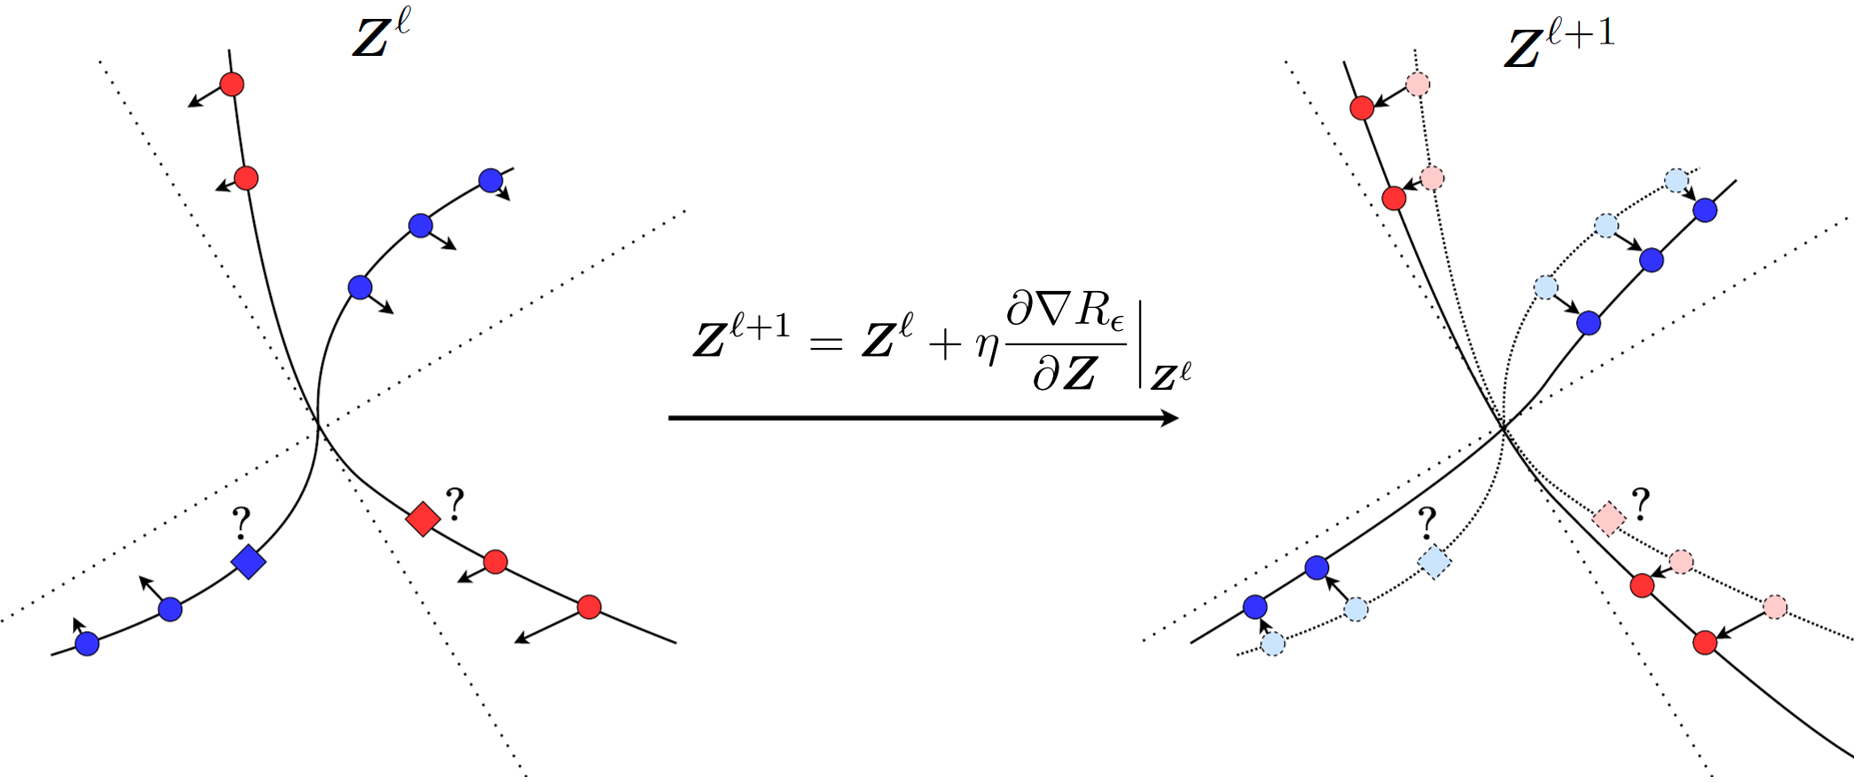
\includegraphics[width=0.85\linewidth]{figs_chap4/redu_gradient_diagram.png}
    \caption{通过梯度流进行增量变形,既将每个类的数据压平到一个子空间,又将不同类推开。}
    \label{fig:gradient-flow}
\end{figure}

% \subsection{从 ReduNet 到 CRATE 的过渡 (待办)}

简单的计算表明,梯度 ${\partial \Delta R_{\epsilon}}/{\partial \bm Z}$ 需要计算 $\Delta R_{\epsilon}$ 中两项的以下导数:
\begin{equation}\label{eqn:expand-directions}
    \frac{1}{2}\frac{\partial \log \det (\I \!+\! \alpha \Z \Z^{\top} )}{\partial \bm Z}\bigg|_{\Z^\ell} = \,\, \underbrace{\alpha(\I \!+\! \alpha\Z^\ell (\Z^\ell)^\top)^{-1}}_{\bm E^{\ell} \; \in \Re^{d\times d}}\Z^\ell,
\end{equation}

\begin{equation}\label{eqn:compress-directions}
\frac{1}{2}\frac{\partial \left( \gamma_{k}  \log \det (\I + \alpha_{k} \Z \bm \Pi_k \Z^{\top} )  \right)}{\partial \bm Z}\bigg|_{\Z^\ell} \\= \gamma_{k}  \underbrace{ \alpha_{k}  (\I +  \alpha_{k} \Z^\ell \bm \Pi_k (\Z^\ell)^{\top})^{-1}}_{\bm C^{\ell}_k \; \in \Re^{d\times d}} \Z^{\ell} \bm \Pi_k.
\end{equation}
请注意,在上述公式中,矩阵 $\bm E^{\ell}$ 仅依赖于 $\Z^{\ell}$,其目的是{\em 扩展}所有特征以增加整体编码率;矩阵 $\bm C^{\ell}_{k}$ 依赖于来自第 $k$ 类的特征,其目的是{\em 压缩}它们以减少每个类的编码率。
那么,完整的梯度 $\frac{\partial \Delta R_{\epsilon}}{\partial \bm Z}\big|_{\Z^\ell} \in \Re^{d\times N}$ 的形式为:
\begin{equation}
\frac{\partial \Delta R_{\epsilon}}{\partial \bm Z}\bigg|_{\Z^\ell}  = \underbrace{\bm E^{\ell}}_{\text{扩展}} \Z^{\ell} \;-\; \sum_{k=1}^K \gamma_{k} \underbrace{\bm C_{k}^{\ell}}_{\text{压缩}}  \Z^{\ell} \bm{\Pi}_k.
\label{eqn:DR-gradient}
\end{equation}

\begin{remark}[$\bm E^\ell$ 和 $\bm C_j^\ell$ 作为线性算子的解释]\label{rem:regression-interpretation}
对于任何 $\bm z^\ell \in \mathbb{R}^d$,
\begin{gather}
    \bm E^\ell \bm z^\ell = \alpha(\bm z^\ell - \bm Z^\ell \bm q^\ell_\star),\
    \mbox{其中}\ \bm q^\ell_\star \doteq \argmin_{\bm q^\ell} \alpha \|\bm z^\ell - \bm Z^\ell \bm q^\ell\|_2^2 + \|\bm q^\ell\|_2^2.
\end{gather}
请注意,$\bm q^\ell_\star$ 正是所有数据点 $\bm Z^\ell$ 的岭回归解。因此,$\bm E^\ell$($\bm C^\ell_k$ 也类似)近似于(即,当 $N$ 足够大时)到由 $\bm Z^\ell$ 的列张成的子空间的正交补空间上的投影。另一种解释矩阵 $\bm E^\ell$ 的方法是通过协方差矩阵 $\Z^\ell (\Z^\ell)^\top$ 的特征值分解。假设 $\Z^\ell (\Z^\ell)^\top \doteq \bm U^\ell \bm \Lambda^\ell (\bm U^\ell)^\top$,其中 $\bm \Lambda^\ell \doteq \diag\left(\lambda^\ell_1, \ldots, \lambda^\ell_d \right)$,我们有
\begin{equation}
\bm E^\ell = \alpha \bm U^\ell\, \diag\left(\frac{1}{1+\alpha\lambda^\ell_1}, \ldots, \frac{1}{1+\alpha\lambda^\ell_d}\right) \left(\bm U^\ell\right)^\top.
\end{equation}
因此,矩阵 $\bm E^\ell$ 对向量 $\bm z^\ell$ 的操作方式是,在方差大的方向上收缩,而在方差小的方向上保持不变。这些正是我们在 \eqref{eqn:expand-directions} 中移动特征的方向,以便整体体积扩大,编码率增加,因此是正号。相反,与 \eqref{eqn:compress-directions} 相关的方向是每个类的特征偏离其应属子空间的“残差”。这些正是特征需要被压缩回各自子空间的方向,因此是负号(见图 \ref{fig:regression-interpretation})。

\begin{figure}[t]
    \centering
    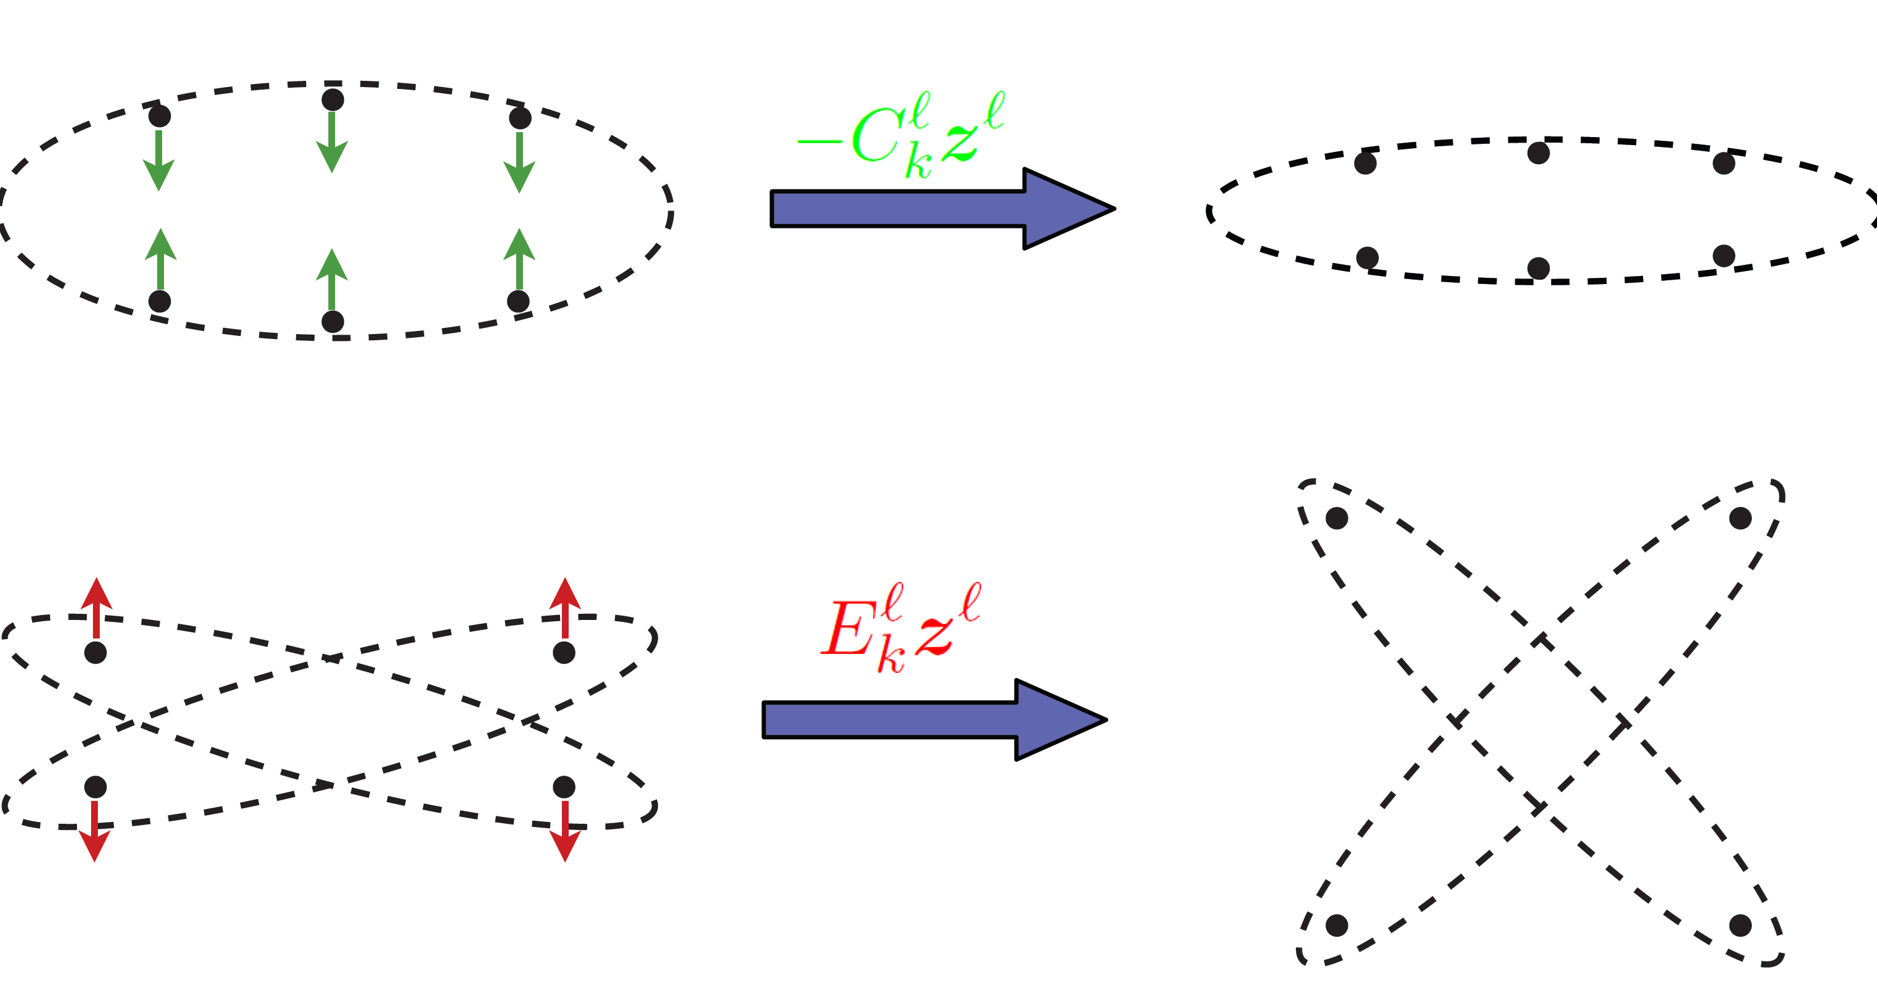
\includegraphics[width=0.65\linewidth]{figs_chap4/expand_compress.png}
    \caption{\small $\bm C^\ell_k$ 和 $\bm E^\ell$ 的解释:$\bm C^\ell_k$ 通过将特征收缩到低维子空间来压缩每个类;$\bm E^\ell$ 通过对比和排斥不同类的特征来扩展所有特征。}
    \label{fig:regression-interpretation}
    \vspace{-0.1in}
\end{figure}


本质上,用于率缩减的梯度上升中的线性操作 $\bm E^\ell$ 和 $\bm C_k^\ell$ 是由训练数据进行“自回归”决定的。最近对过参数化设置中岭回归的新理解 \cite{yang2020rethinking,Wu2020OnTO} 表明,使用看似冗余的采样数据(来自每个子空间)作为回归量并不会导致过拟合。
\end{remark}

\paragraph{梯度引导的特征图增量。} 请注意,在上述内容中,梯度上升将所有特征 $\Z^{\ell} = [\z^{\ell}_{1}, \dots, \z^{\ell}_{N}]$ 视为自由变量。增量 $\Z^{\ell+1} - \Z^{\ell} = \eta \frac{\partial \Delta R_{\epsilon}}{\partial \bm Z}\big|_{\Z^\ell}$ 尚未给出对整个特征域 $\z^\ell \in \Re^d$ 的变换。根据方程 \eqref{eqn:DR-gradient},梯度无法在隶属关系未知的点上评估,如图 \ref{fig:gradient-flow} 所示。因此,为了明确地找到最优的 $f(\x,\bm  \theta)$,我们可以考虑在第 $\ell$ 层的特征 $\z^\ell$ 上构造一个小的增量变换 $g(\cdot, \bm{\theta}^{\ell})$ 来模拟上述(投影)梯度方案:
\begin{equation}
\z^{\ell + 1}   \; \propto \; \z^{\ell} + \eta\cdot  g(\z^{\ell}, \bm{\theta}^{\ell}) \quad \mbox{subject to} \quad \z^{\ell +1} \in \mathbb{S}^{d-1}
\label{eqn:gradient-descent-transform}
\end{equation}
使得 $\big[g(\z_1^{\ell}, \bm \theta^{\ell}), \ldots, g(\z_N^{\ell}, \bm \theta^{\ell}) \big] \approx \frac{\partial \Delta R_{\epsilon}}{\partial \bm Z}\big|_{\Z^\ell}$。也就是说,我们需要用一个在整个特征空间 $\z^\ell \in \Re^d$ 上定义的连续映射 $g(\z,\bm \theta)$ 来近似局部变形所有(训练)特征 $\{\z_i^\ell\}_{i=1}^N$ 的梯度流 $\frac{\partial \Delta R_{\epsilon}}{\partial \bm Z}$。
请注意,人们可以将增量 \eqref{eqn:gradient-descent-transform} 解释为连续微分方程的离散化版本:
\begin{equation}
\dot{\z} = g(\z, \theta).
\end{equation}
因此,如此构建的(深度)网络可以被解释为某种神经 ODE \cite{chen2018neural}。然而,与神经 ODE 中流 $g$ 被选择为某些通用结构不同,这里的 $g(\z, \bm\theta)$ 是为了模拟特征集上率缩减的梯度流(如图 \ref{fig:gradient-flow} 所示):
\begin{equation*}
    \dot{\Z} = \frac{\partial \Delta R_{\epsilon}}{\partial \bm Z},
\end{equation*}
并且其结构完全是从这个目标推导和确定的,没有任何其他先验或启发式方法。

通过检查梯度 \eqref{eqn:DR-gradient} 的结构,它表明增量变换 $g(\z^\ell, \bm \theta^\ell)$ 的一个自然候选形式是:
\begin{equation}
    g(\z^\ell, \bm \theta^\ell) \; \doteq \; \bm E^\ell \z^\ell - \sum_{k=1}^K \gamma_{k} \pi_k(\z^\ell)\bm C_{k}^{\ell}  \z^{\ell}  \in \Re^d,
    \label{eqn:DR-gradient-transform}
\end{equation}
其中 $\pi_k(\z^\ell) \in [0,1]$ 表示 $\z^{\ell}$ 属于第 $k$ 类的概率。增量映射参数 $\bm \theta^\ell$ 依赖于:首先,一组由 $\bm E^{\ell}$ 和 $\{ \bm C^{\ell}_{k}\}_{k=1}^{K}$ 表示的线性映射,它们仅依赖于训练特征 $\Z^\ell$ 的统计量;其次,任何特征 $\z^\ell$ 的隶属关系 $\{ \pi_k(\z^\ell)\}_{k=1}^K$。
请注意,在训练样本 $\Z^\ell$ 上,其隶属关系 $\bm \Pi_k$ 是已知的,如此定义的 $g(\z^\ell, \bm \theta)$ 恰好给出了梯度 $\frac{\partial \Delta R_{\epsilon}}{\partial \bm Z}\big|_{\Z^\ell}$ 的值。


由于我们只知道训练样本的隶属关系,因此在 \eqref{eqn:DR-gradient-transform} 中定义的函数 $g(\cdot)$ 只能在训练集上评估。为了将 $g(\cdot)$ 外推到整个特征空间,我们需要估计其第二项中的 $\pi_k(\z^\ell)$。在传统的深度学习中,这个映射通常被建模为一个深度网络,并从训练数据中学习,例如通过{\em 反向传播}。然而,我们这里的目标还不是学习一个精确的分类器 $\pi_{k}(\z^\ell)$。相反,我们只需要一个足够好的类别信息估计,以便 $g(\cdot)$ 能够很好地近似梯度 $\frac{\partial \Delta R_{\epsilon}}{\partial \bm Z}$。



从备注 \ref{rem:regression-interpretation} 给出的线性映射 $\bm E^\ell$ 和 $\bm C_k^\ell$ 的几何解释来看,项 $\bm p_{k}^{\ell} \doteq \bm C^{\ell}_k \z^{\ell}$ 可以被看作是(近似地)$\z^{\ell}$ 在每个类 $j$ 的正交补空间上的投影。因此,如果 $\z^\ell$ 属于类 $j$,则 $\|\bm p_{j}^{\ell}\|_2$ 很小,否则很大。这启发我们基于以下 softmax 函数来估计其隶属关系:
\begin{equation}
    \widehat{\vpi}(\z^\ell) \doteq \softmax\rp{-\lambda\mat{\norm{\vC^{\ell}_{1}\vz^{\ell}}_{2} \\ \vdots \\ \norm{\vC^{\ell}_{K}\vz^{\ell}}_{2}}} = \frac{1}{\sum_{k = 1}^{K}\exp(-\lambda \norm{\vC^{\ell}_{k}\vz^{\ell}}_{2})}\mat{\exp(-\lambda\norm{\vC^{\ell}_{1}\vz^{\ell}}_{2}) \\ \vdots \\ \exp(-\lambda\norm{\vC^{\ell}_{K}\vz^{\ell}}_{2})} \in [0,1]^{K}.
\end{equation}
因此,\eqref{eqn:DR-gradient-transform} 的第二项可以通过这个估计的隶属关系来近似:
\begin{align}
\sum_{k=1}^K \gamma_{k} \pi_k(\z^\ell)\bm C_{k}^{\ell}  \z^{\ell} 
\; \approx \;  \sum_{k=1}^K \gamma_{k} \widehat{\pi}_k(\z^\ell)  \bm{C}^{\ell}_k  \z^{\ell} 
\; \doteq \; \bm \sigma\Big([\bm{C}^{\ell}_{1} \z^{\ell}, \dots, \bm{C}^{\ell}_{K} \z^{\ell}]\Big),
\label{eqn:soft-residual}
\end{align}
这被表示为一个非线性算子 $\bm \sigma(\cdot)$,作用于特征 $\z^\ell$ 通过 $K$ 组滤波器 $[\bm{C}^{\ell}_{1}, \dots, \bm{C}^{\ell}_{K}]$ 的输出。请注意,非线性是由于基于这些滤波器响应的类别隶属关系的“软”分配而产生的。

总的来说,结合 \eqref{eqn:gradient-descent-transform}、\eqref{eqn:DR-gradient-transform} 和 \eqref{eqn:soft-residual},
从 $\z^{\ell}$ 到 $\z^{\ell+1}$ 的增量特征变换现在变为
\begin{equation}\label{eqn:layer-approximate}
\begin{aligned}
\z^{\ell+1}  &\propto \; \z^\ell +  \eta \cdot  \bm E^{\ell} \z^{\ell} - \eta\cdot  \bm \sigma\big([\bm{C}^{\ell}_{1} \z^{\ell}, \dots, \bm{C}^{\ell}_{K} \z^{\ell}]\big)  \\
&= \; \z^\ell +  \eta \cdot g(\z^\ell, \bm \theta^\ell) \qquad \mbox{s.t.} \quad \z^{\ell +1} \in \mathbb{S}^{d-1},
\end{aligned}
\end{equation}
其中非线性函数 $\bm \sigma(\cdot)$ 如上定义,$\bm \theta^\ell$ 收集了所有层级参数。即 $\bm \theta^\ell =\left\{\bm E^\ell, \bm{C}^{\ell}_{1}, \dots, \bm{C}^{\ell}_{K}, \gamma_{k}, \lambda\right\}$。注意,每一层的特征总是通过投影到单位球面 $\mathbb S^{d-1}$ 上来进行“归一化”,记为 $\mathcal P_{\mathbb S^{d-1}}$。\eqref{eqn:layer-approximate} 中的增量形式可以用图 \ref{fig:arch-ReduNet}(a) 中的图表来说明。

\begin{figure}[t]
    \begin{subfigure}[t]{0.35\textwidth}
        \centering
        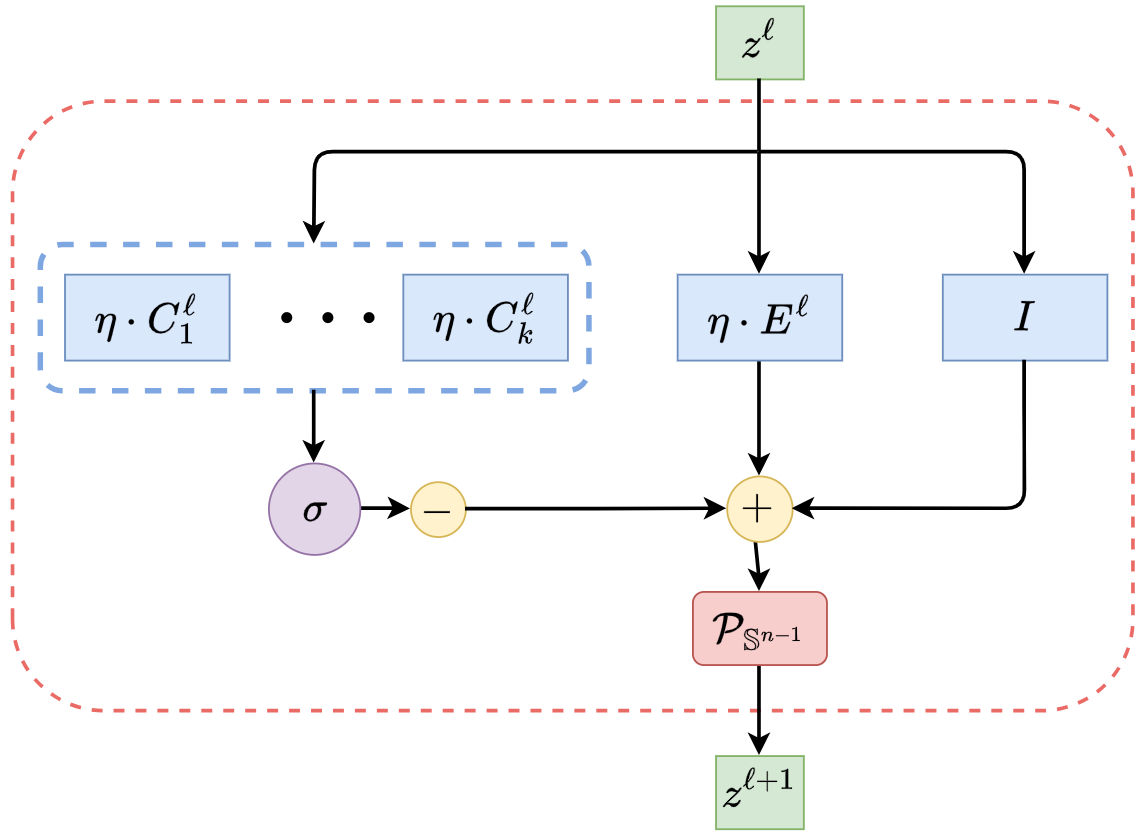
\includegraphics[width=\textwidth]{figs_chap4/redunet_layer.png}
        \caption{\textbf{ReduNet}}
    \end{subfigure}
    \hfill
    \begin{subfigure}[t]{0.6\textwidth}
        \centering
        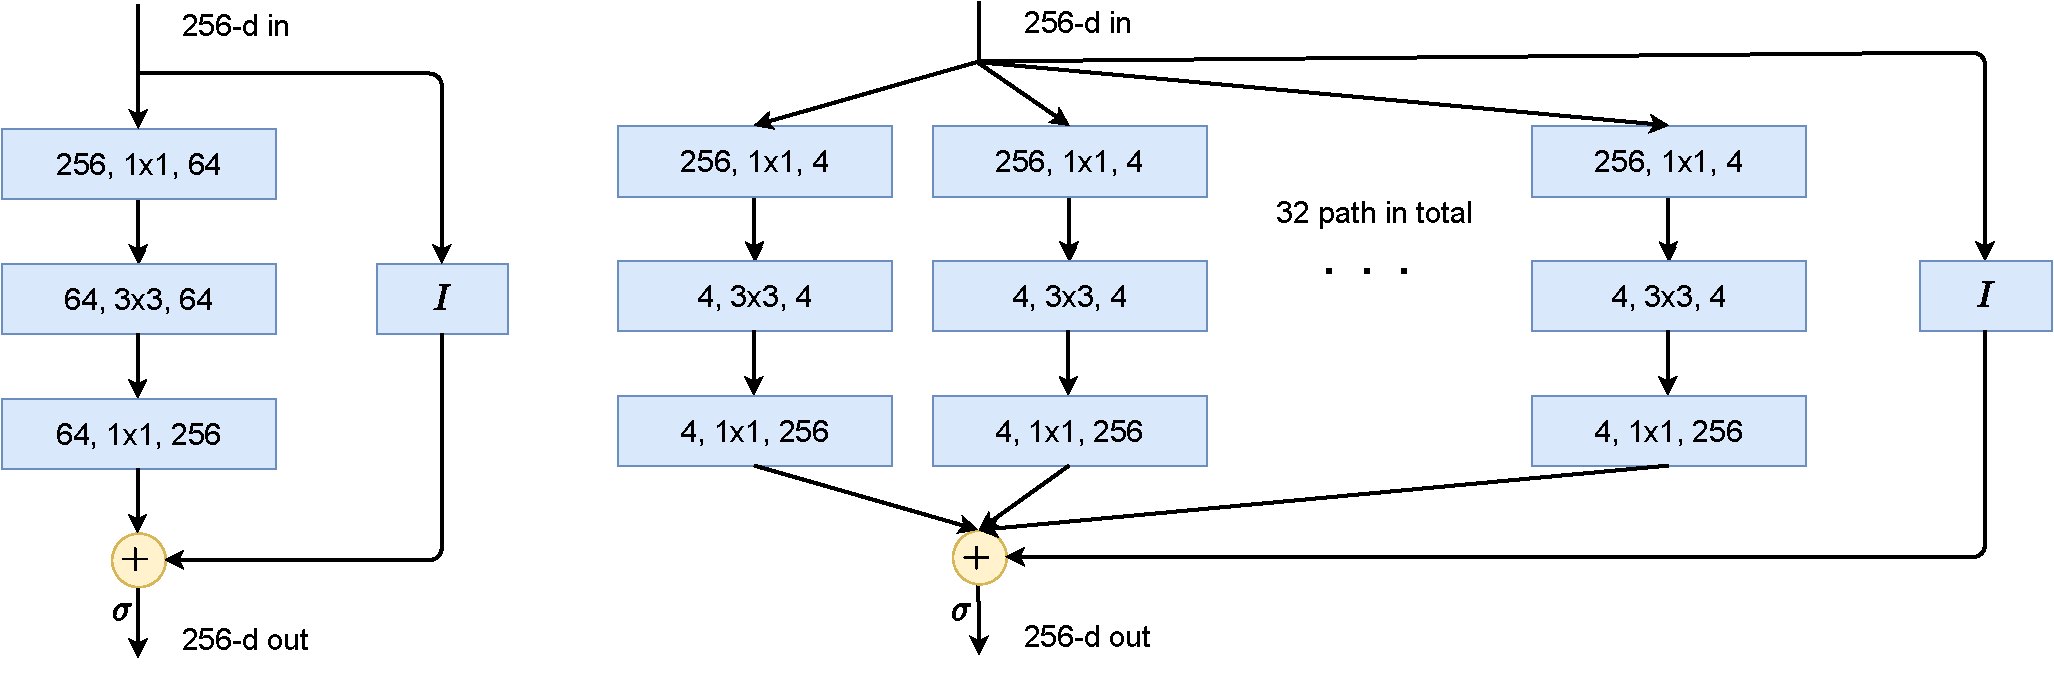
\includegraphics[width=\textwidth]{figs_chap4/resnet_resnext.pdf}
        \caption{\textbf{ResNet} 和 \textbf{ResNeXt}。}
    \end{subfigure}
    \caption{\small ReduNet 的网络架构及与其他架构的比较。\textbf{(a)}:从优化率缩减的一次梯度上升迭代中推导出的 \textbf{ReduNet} 的层结构。\textbf{(b)} (左):ResNet~\cite{he2016deep} 的一层;以及 \textbf{(b)} (右):ResNeXt~\cite{ResNEXT} 的一层。正如我们将在第 \ref{sec:shift-invariant} 节中看到的,当施加平移不变性时,ReduNet 的线性算子 $\bm E^\ell$ 和 $\bm{C}_k^\ell$ 自然地变成(多通道)卷积。}
    \label{fig:arch-ReduNet}
\end{figure}

\begin{algorithm}[t]
    \caption{ReduNet 的训练算法}
    \label{alg:redunet_training}
    \begin{algorithmic}[1]
        \Require{$\vX = [\vx_1, \ldots, \vx_N]\in \Re^{D \times N}$,$\bm{\Pi} = \{\bm \Pi_k\}_{k=1}^K$,$\epsilon > 0$,$\lambda$ 和学习率 $\eta$。}
        \Ensure{学习到的参数 \(\{\vE^{\ell}\}_{\ell = 1}^{L}, \{\{\vC^{\ell}_{k}\}_{k = 1}^{K}\}_{\ell = 1}^{L}, \{\gamma_{k}\}_{k = 1}^{k}\)}

        \Procedure{ReduNetTraining}{$\vX, \vPi, \epsilon, \lambda, \eta$}
            \Statex{\quad\ \texttt{\# 定义常量}}

            \State{\(\alpha \gets d/(N\epsilon^{2})\)}
            \For{\(k \in \{1, \dots, K\}\)}
            \State{\(\alpha_{k} \gets D/(\tr(\vPi_{k})\epsilon^{2})\)}
            \State{\(\gamma_{k} \gets \tr(\vPi_{k})/D\)}
            \EndFor
            \Statex{}

            \Statex{\quad\ \texttt{\# ReduNet 逐层迭代}}
            \State{\(\vZ^{1} = \mat{\vz_{1}^1, \dots, \vz_{N}^1} \gets \vX\)} \Comment{初始化 ReduNet 的逐层迭代}
            \For{\(\ell \in \{1, \dots, L\}\)}
                \Statex{\quad\ \texttt{\# 步骤 1: 计算网络参数} \(\vE^{\ell}, \{\vC^{\ell}_{k}\}_{k = 1}^{K}\)}
                \State{\(\vE^{\ell} \gets \alpha\left(\vI + \alpha \vZ^{\ell}(\vZ^{\ell})^{\top}\right)^{-1} \in \R^{d \times d}\)}
                \For{\(k \in \{1, \dots, K\}\)}
                    \State{\(\vC^{\ell}_{k} \gets \alpha_{k}\left(\vI + \alpha_{k}\vZ^{\ell}\vPi_{k}(\vZ^{\ell})^{\top}\right)^{-1} \in \R^{d \times d}\)}
                \EndFor
                \Statex{}
                \Statex{\qquad\quad\texttt{\# 步骤 2: 更新特征 \(\vZ^{\ell}\)}}
                \For{\(i \in \{1, \dots, N\}\)}
                    \State{\(\hat{\vpi}(\vz^{\ell}_i) \gets \displaystyle \softmax(-\lambda[\norm{\vC^{\ell}_{1}\vz^{\ell}_i}_{2}, \dots, \norm{\vC^{\ell}_{K}\vz^{\ell}_i}_{2}]) \in [0, 1]^{K}\)} \Comment{计算软分配 \(\hat{\vpi}(\vz^{\ell}_i)\)}
                    \State{\(\displaystyle\vz^{\ell + 1}_i \gets \cP_{\bS^{d - 1}}\rp{\vz^{\ell}_i + \eta \bp{\vE^{\ell}\vz^{\ell}_i - \sum_{k = 1}^{K}\gamma_{k}\hat{\pi}_{k}(\vz^{\ell}_i) \vC^{\ell}_{k}\vz^{\ell}_i}} \in \R^{d}\)} \Comment{从 \(\vz^{\ell}_i\) 更新特征 \(\vz^{\ell + 1}_i\)}
                \EndFor
            \EndFor
            \State{\Return{\(\{\vE^{\ell}\}_{\ell = 1}^{L}, \{\{\vC^{\ell}_{k}\}_{k = 1}^{K}\}_{\ell = 1}^{L}, \{\gamma_{k}\}_{k = 1}^{K}\)}} \Comment{返回所有网络参数。}
        \EndProcedure
    \end{algorithmic}
\end{algorithm}


\paragraph{用于优化率缩减的深度网络。} 请注意,增量是为了模拟率缩减 $\Delta R_\epsilon$ 的梯度上升而构建的。因此,通过上述过程迭代地变换特征,我们期望率缩减会增加,正如我们将在实验部分看到的那样。这个迭代过程,一旦收敛(比如说经过 $L$ 次迭代),就给出了输入 $\x = \z^0$ 上期望的特征映射 $f(\x, \bm \theta)$,其形式恰好是一个{\em 深度网络},其中每一层都具有图 \ref{fig:arch-ReduNet} 左侧所示的结构:
\begin{equation}\label{eqn:ReduNet}
\begin{aligned}
f(\x, \bm \theta)\; =&  \;\;f^L \circ f^{L-1} \circ  \cdots \circ f^1 \circ
    f^0(\z^0),  \\
f^\ell(\z^\ell, \bm \theta^\ell) \; \doteq & \;\; \z^{\ell+1} = \mathcal{P}_{\mathbb{S}^{n-1}}[\z^{\ell} + \eta\cdot g(\z^{\ell}, \bm \theta^{\ell})], \\
g(\z^{\ell}, \bm \theta^{\ell}) \; =&\;\; \bm E^{\ell} \z^{\ell} -  \bm \sigma\big([\bm{C}^{\ell}_{1} \z^{\ell}, \dots, \bm{C}^{\ell}_{K} \z^{\ell}]\big).
\end{aligned}
\end{equation}
由于这个深度网络是从最大化率\textbf{缩减}(rate \textbf{redu}ction)推导出来的,我们称之为 \textbf{ReduNet}。通过将 ReduNet 的架构与流行的经验设计网络,如图 \ref{fig:arch-ReduNet} 所示的 \textbf{ResNet} 和 \textbf{ResNeXt} 进行比较,其相似性有些惊人。从概念上讲,ReduNet 也可以用来证明流行的混合专家(\textbf{MoE})架构 \cite{MoE} 的合理性,因为每个并行通道 $\bm{C}^{\ell}_k$ 都可以被看作是为每个对象类别训练的“专家”。

\begin{figure}[t]
    \centering
    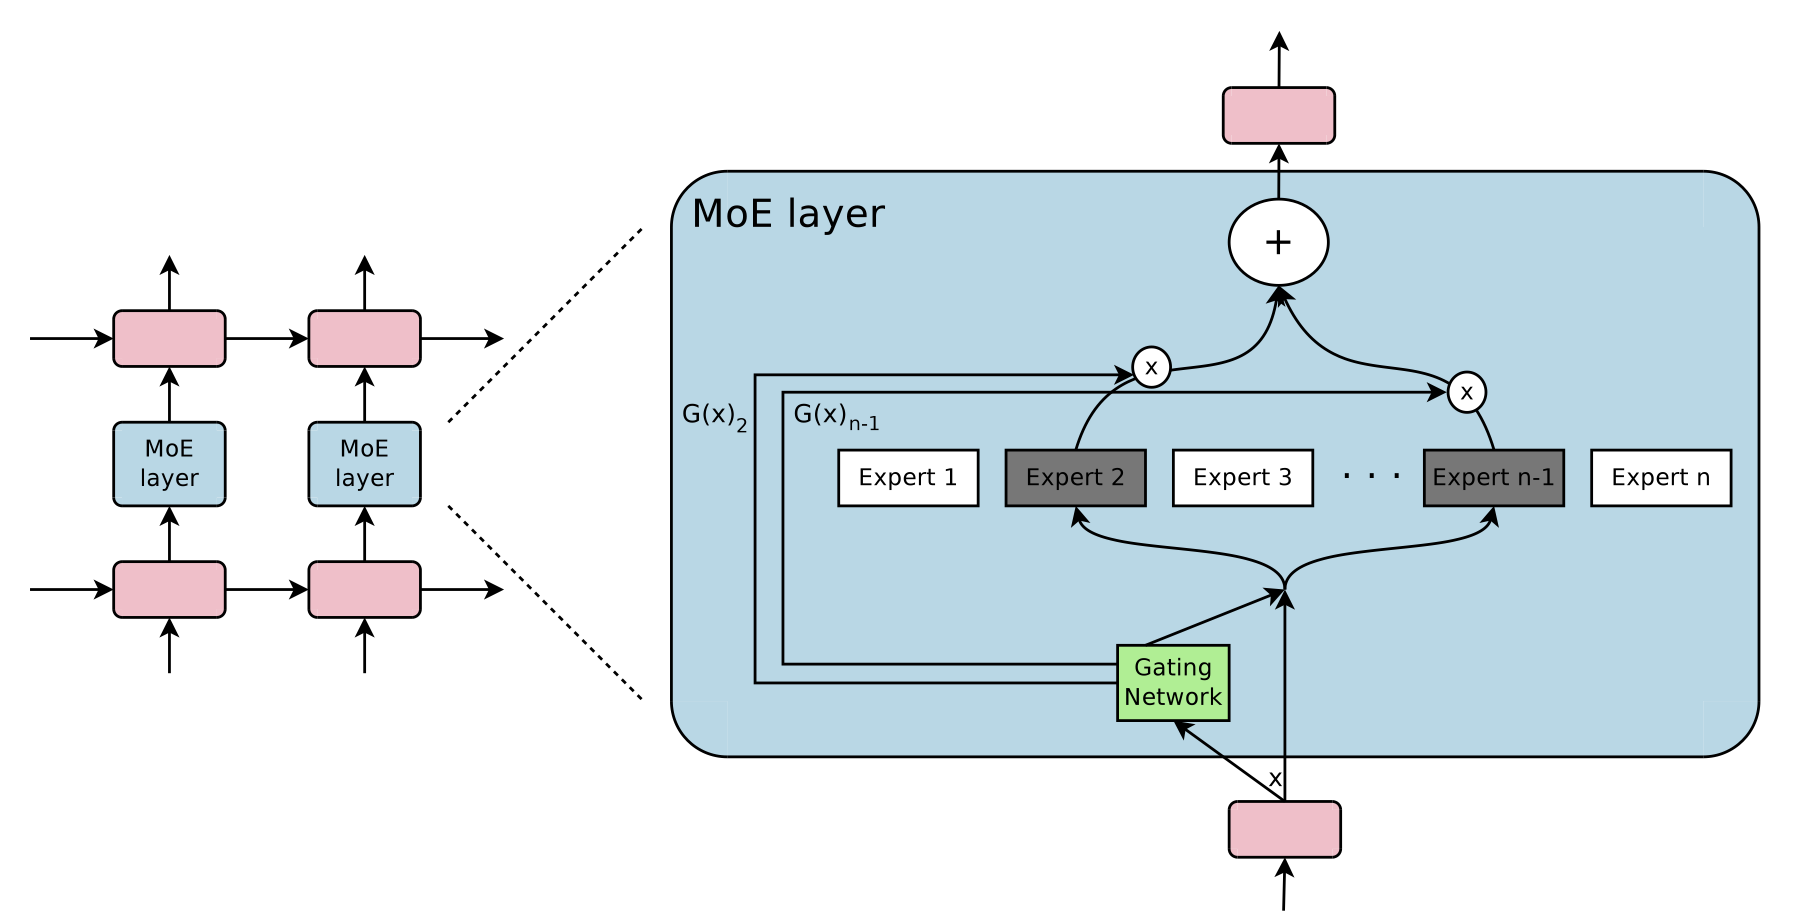
\includegraphics[width=0.45\linewidth]{figs_chap4/MoE.png} \hspace{5mm}
    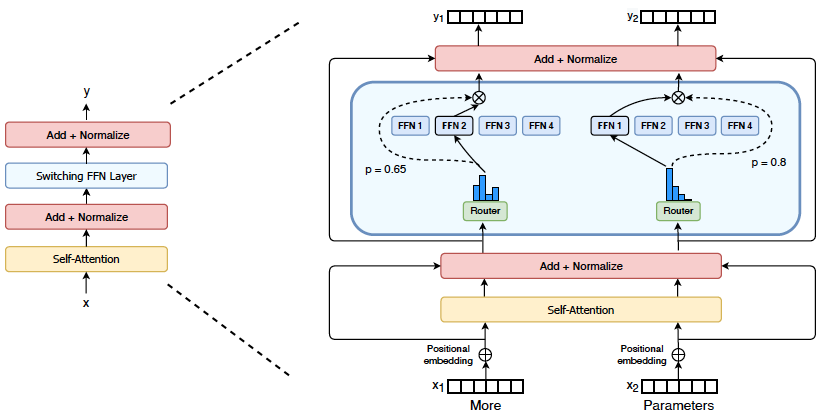
\includegraphics[width=0.45\linewidth]{figs_chap4/switched-transformer.png}
    \caption{左:一个混合专家(MoE)深度网络 \cite{MoE}。右:一个促进稀疏性的 Switch Transformer \cite{Fedus-2022},用于实现具有 1.7 万亿参数的 MoE。}
    \label{fig:enter-label}
\end{figure}

我们在 \Cref{alg:redunet_training} 和 \Cref{alg:redunet_evaluation} 中分别总结了 ReduNet 的训练和评估。请注意,网络的所有参数都是以{\em 前向传播}的方式逐层显式构建的。这种构建不需要任何反向传播!如此学习到的特征可以直接用于分类,例如通过最近子空间分类器。
% \yima{一些仿真例子,就像我们在论文中用球面上的三个簇做的那样?例子对于教学很重要!} \yaodong{在下面添加了图 \ref{fig:redu-3d-gaussian-diagram} 和一段文字。}



\begin{algorithm}[!htbp]
    \caption{ReduNet 的评估算法}
    \label{alg:redunet_evaluation}
    \begin{algorithmic}[1]
        \Require{输入 \(\vx \in \R^{D}\),网络参数 \(\{\vE^{\ell}\}_{\ell = 1}^{L}, \{\{\vC^{\ell}_{k}\}_{k = 1}^{K}\}_{\ell = 1}^{L}, \{\gamma_{k}\}_{k = 1}^{K}\),学习率 \(\lambda\)}
        \Ensure{特征 \(\vz^{L + 1}\)}

        \Procedure{ReduNetEvaluation}{$\vx$}
        \State{\(\vz^{1} \gets \vx \in \R^{D}\)} \Comment{初始化 ReduNet 的逐层迭代}
        \For{\(\ell \in \{1, \dots, L\}\)}
        \State{\(\hat{\vpi}(\vz^{\ell}) \gets  \softmax(-\lambda\mat{\norm{\vC^{\ell}_{1}\vz^{\ell}}_{2}, \dots, \norm{\vC^{\ell}_{K}\vz^{\ell}}_{2}}) \in [0, 1]^{K}\)} \Comment{计算软分配 \(\hat{\vpi}(\vz^{\ell})\)}
        \State{\(\vz^{\ell + 1} \gets \cP_{\bS^{d - 1}}\rp{\vz^{\ell} + \eta \bp{\vE^{\ell}\vz^{\ell} - \sum_{k = 1}^{K}\gamma_{k}\hat{\pi}_{k}(\vz^{\ell}) \vC^{\ell}_{k}\vz^{\ell}}} \in \R^{d}\)} \Comment{使用 \(\vz^{\ell}\) 更新特征 \(\vz^{\ell + 1}\)}
        \EndFor
        \State{\Return{\(\vz^{L + 1}\)}} \Comment{返回输出特征}
        \EndProcedure
    \end{algorithmic}
\end{algorithm}


\begin{example}
为了提供一些关于 ReduNet 如何变换特征的直观理解,我们提供一个混合 3D 高斯分布的简单例子,并在图 \ref{fig:redu-3d-gaussian-diagram} 中可视化特征是如何变换的。
考虑一个在 $\R^{3}$ 中混合的三个高斯分布,并将其投影到 $\mathbb{S}^2$ 上。我们首先为 3 个类别生成数据点:对于 $k=1,2,3$,$\bm{X}_{k}=[\bm{x}_{k,1}, \ldots, \bm{x}_{k,m}] \in \R^{3\times m}$,$\bm{x}_{k,i} \sim \mathcal{N}(\bm{\mu}_{k}, \sigma_{k}^{2} \I)$,且 ${\pi}(\x_{k,i}) = k$。
我们设置 $m=500, \sigma_{1}=\sigma_{2}=\sigma_{3}=0.1$,以及 $\bm{\mu}_{1}, \bm{\mu}_{2}, \bm{\mu}_{3} \in \mathbb{S}^2$。
然后我们将所有数据点投影到 $\mathbb{S}^{2}$ 上,即 $\bm{x}_{k,i}/\|\bm{x}_{k,i}\|_{2}$。
为了构建网络(为第 $\ell$ 层计算 $\bm{E}^{\ell}, \bm{C}^{\ell}_{k}$),我们设置迭代/层数 $L=2,000$,步长 $\eta=0.5$,精度 $\epsilon=0.1$。
我们这样做只是为了证明我们的框架即使有数千层也能得到稳定的深度网络。
在实践中,数千层可能不是必需的,当增加新层带来的回报递减时就可以停止。
对于这个例子,几百层就足够了。因此,明确的优化目标为所需网络的深度提供了一个自然准则。

如图 \ref{fig:redu-3d-gaussian-diagram} 所示,我们可以观察到,经过映射 $f(\cdot, \bm{\theta})$ 后,来自同一类别的样本被高度压缩并收敛到一个单一的簇,而不同簇之间的角度近似为 $\pi/2$,这与 MCR$^2$ 损失在 $\mathbb{S}^2$ 中的最优解 $\Z^{\star}$ 非常吻合。
不同层上特征的 MCR$^2$ 损失可以在图 \ref{fig:redu-3d-gaussian-diagram}(\textbf{c}) 中找到。根据经验,我们发现构建的 ReduNet 能够最大化 MCR$^2$ 损失并稳定收敛,来自同一类别的样本收敛到一个簇,不同簇之间相互正交。
此外,当从相同的分布中采样新的数据点时,我们发现来自同一类别的新样本始终收敛到与训练样本相同的簇中心。
\begin{figure}[t]
    \begin{subfigure}[t]{0.32\textwidth}
        \centering
        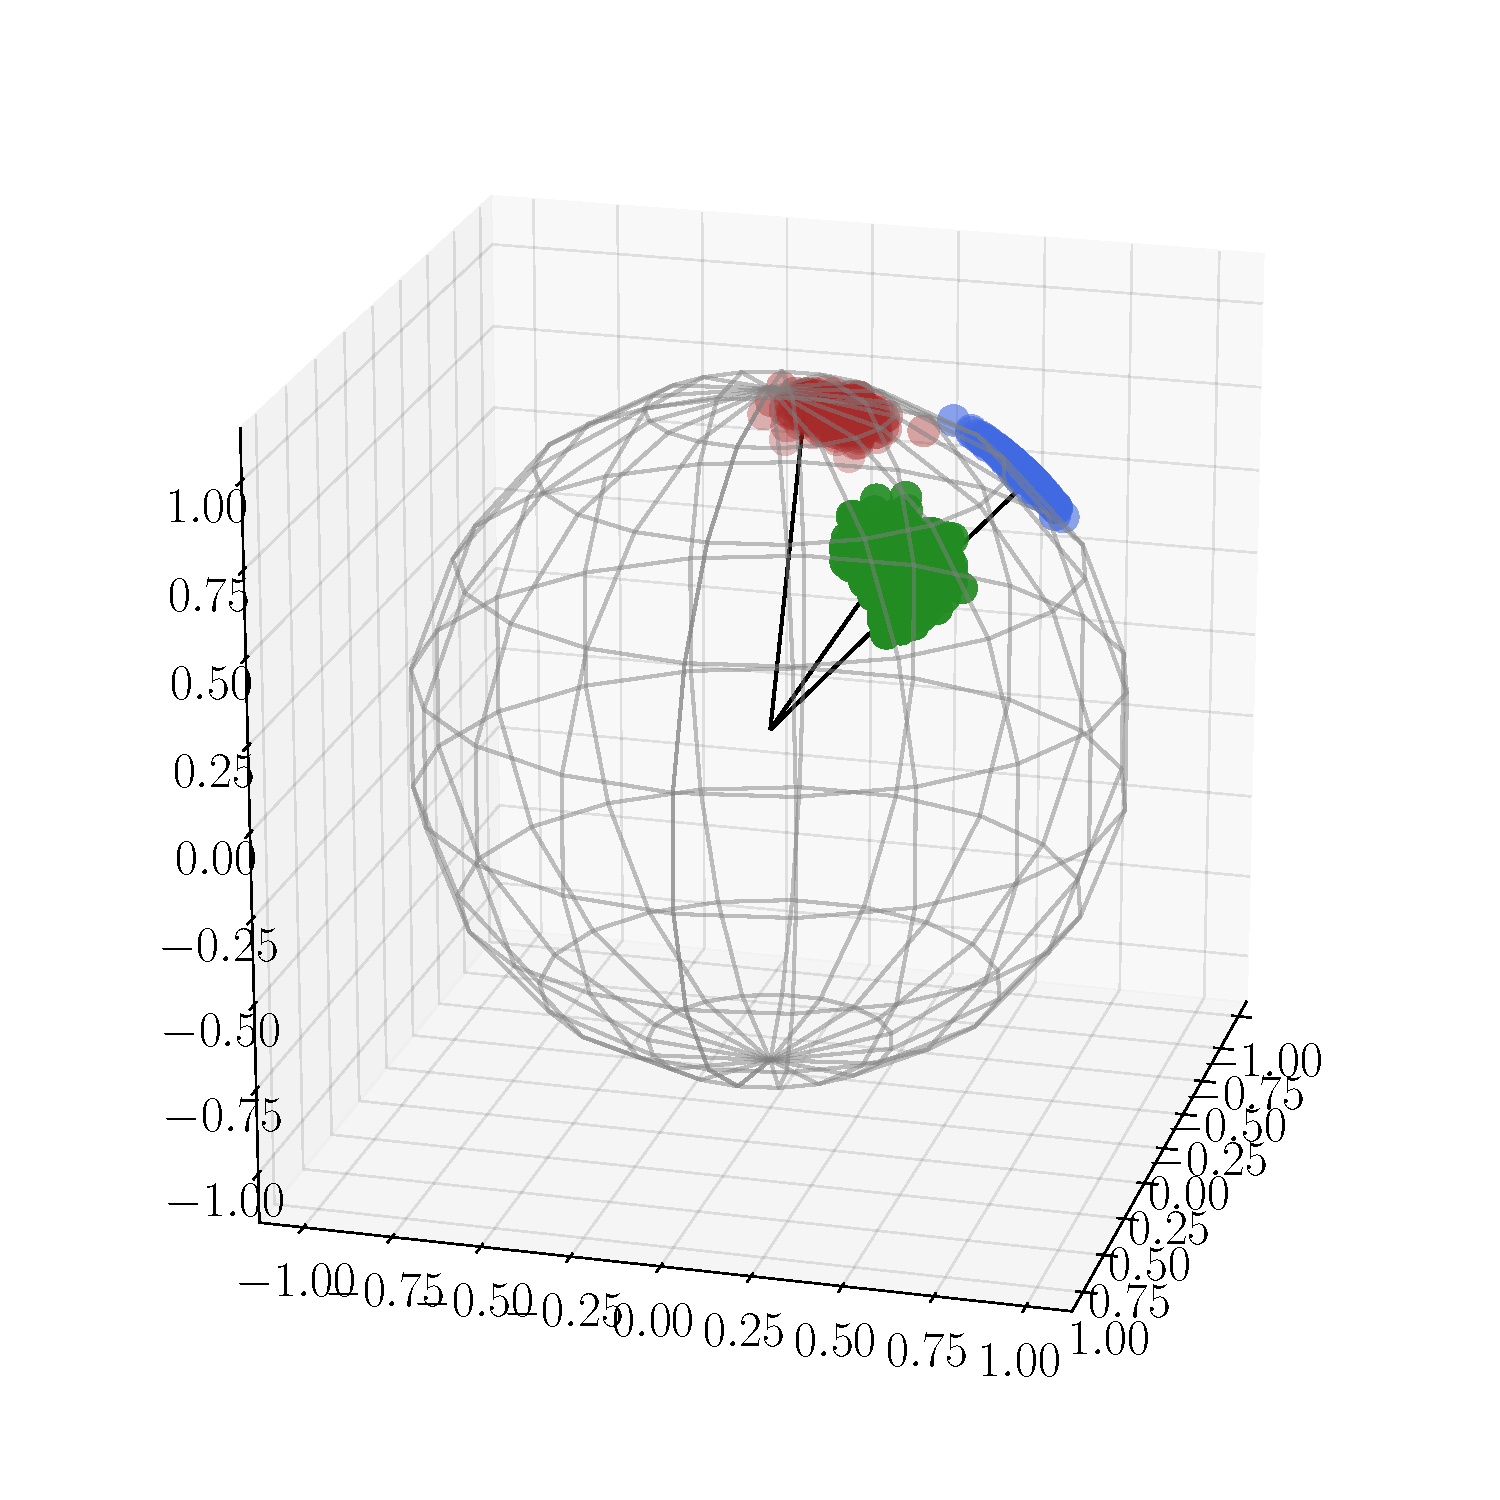
\includegraphics[width=\textwidth]{figs_chap4/scatter3d-X_train.pdf}\vspace{-0.1in}
        \caption{$\bm{X}_{\text{train}}$}
    \end{subfigure}
    \hfill
    \begin{subfigure}[t]{0.32\textwidth}
        \centering
        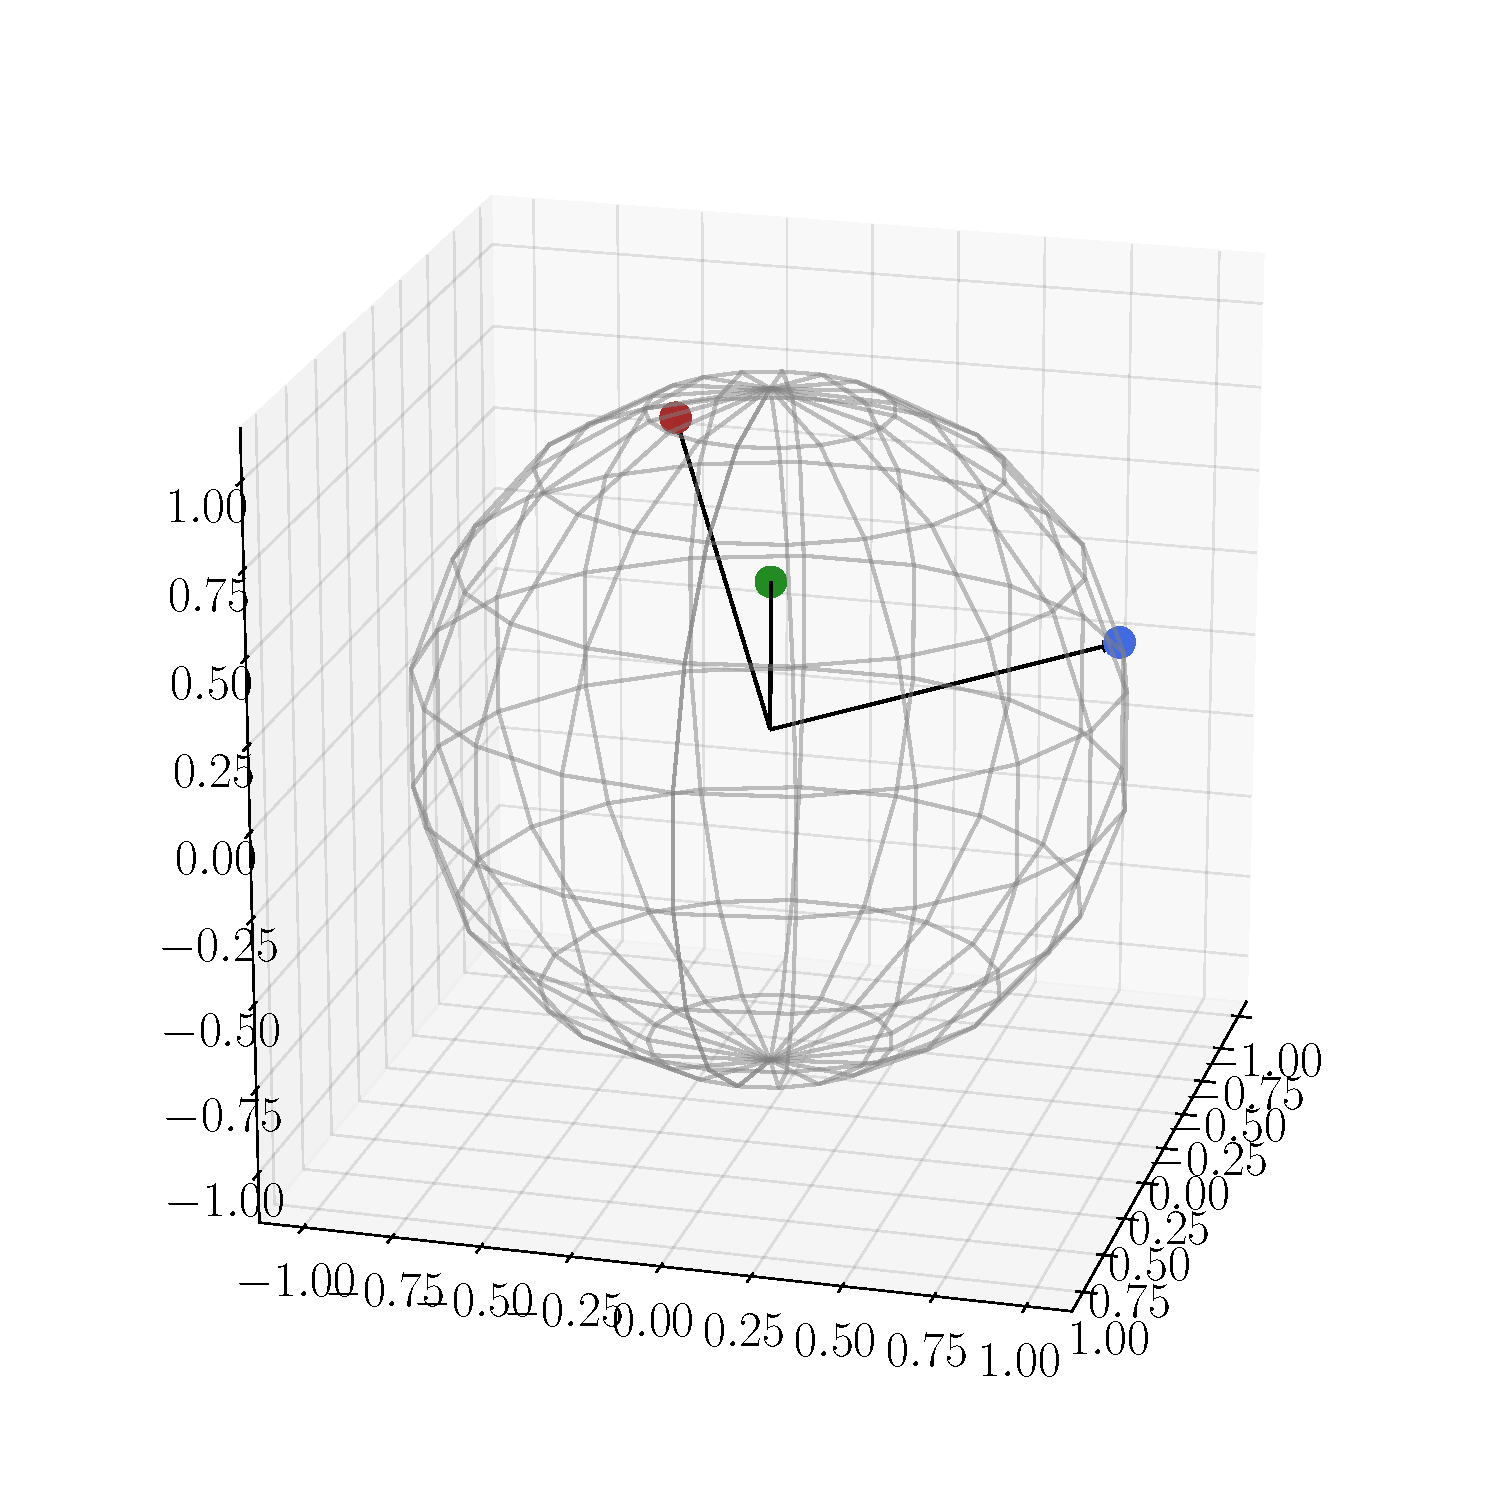
\includegraphics[width=\textwidth]{figs_chap4/scatter3d-Z_train.pdf}\vspace{-0.1in}
        \caption{$\bm{Z}_{\text{train}}$}
    \end{subfigure}
    \hfill
    \begin{subfigure}[t]{0.32\textwidth}
        \centering
        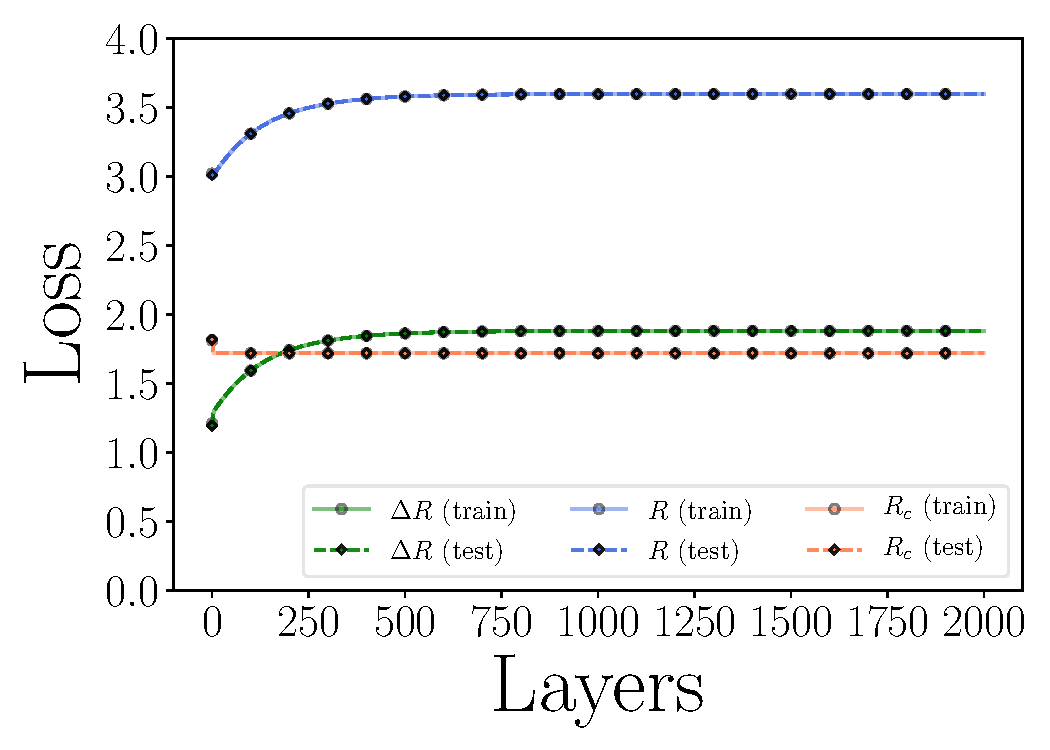
\includegraphics[width=\textwidth]{figs_chap4/scatter3d-loss-traintest.pdf}\vspace{-0.1in}
        \caption{损失 (训练/验证)}
    \end{subfigure}
    \vspace{-0.1in}
    \caption{\small 3D 高斯混合的原始样本和学习到的表示。我们通过散点图在 (\textbf{a}) 中可视化数据点 $\bm{X}$(映射 $f(\cdot, \bm{\theta})$ 之前)和在 (\textbf{b}) 中可视化学习到的特征 $\bm{Z}$(映射 $f(\cdot, \bm{\theta})$ 之后)。在每个散点图中,每种颜色代表一类样本。在 (\textbf{c}) 中,我们还展示了目标函数值的进展图。}
    \label{fig:redu-3d-gaussian-diagram}
\end{figure}

\end{example}

\subsection{来自不变率缩减的卷积网络}\label{sec:shift-invariant}
%\yaodong{待办事项:在这里放一个过渡段落,强调我们可以通过最大化带有数据增强的率缩减来推导出卷积层。我在下面放了一个初始段落(可以随意编辑)。}

在上一节中,我们使用展开优化率缩减目标的方法,推导出了深度网络 ReduNet 的逐层架构。
具体来说,公式 \eqref{eq:mcr-formulation} 中的压缩项 $R^c_\epsilon(\Z \mid\bm \Pi)$ 旨在压缩来自同一类别的表示。然而,这个公式没有考虑输入数据可能存在的域变换或形变。例如,将一个物体稍微向右移动并不会改变图像的语义标签。在本节中,我们将演示如何通过最大化一个对某些域形变(如图像旋转和平移)不变的率缩减目标来推导出卷积层。


对于许多聚类或分类任务(例如图像中的目标检测),如果两个样本之间仅存在某些类别的域形变或数据增强 $\cT = \{\tau \}$,我们就认为它们是{\em 等价的}。因此,我们只对那些对这类形变{\em 不变}的低维结构感兴趣(即,当且仅当对于所有 $\tau \in \cT$,$\tau(\x) \in \mathcal{M}$ 时,$\x \in \mathcal{M}$),
众所周知,这些结构具有复杂的几何和拓扑结构,在实践中可能难以精确学习,即使使用严格设计的 CNN 也是如此 \cite{Cohen-ICML-2016}。
在这个框架中,这可以以一种非常自然的方式来表述:所有等变实例都将被嵌入到同一个子空间中,从而使得子空间本身对所考虑的变换是不变的。

在许多应用中,例如序列数据或图像数据,数据的语义(标签)对某些变换 $\mathfrak{g} \in \mathbb{G}$(对于某个群 $\mathbb{G}$)是{\em 不变的} \cite{CohenW16,deep-sets-NIPS2017}。例如,音频信号的意义对时间上的平移是不变的;图像中物体的身份对图像平面上的平移是不变的。因此,我们希望特征映射 $f(\x,\bm \theta)$ 对这类变换是严格不变的:
\begin{equation}
\mbox{\em 群不变性:}\;   f(\x\circ \mathfrak{g}, \bm \theta) \sim f(\x,\bm \theta),\ \forall \mathfrak{g} \in \mathbb{G},
\end{equation}
其中“$\sim$”表示两个特征属于同一个等价类。尽管为了确保不变性或等变性,卷积算子在深度网络中已是常见做法 \cite{CohenW16},但在实践中,从头开始训练一个(经验设计的)卷积网络以{\em 保证}对简单变换(如平移和旋转)的不变性仍然具有挑战性 \cite{azulay2018deep,engstrom2017rotation}。另一种方法是仔细设计每一层的卷积滤波器,以确保对各种信号的平移不变性,例如在 ScatteringNet \cite{scattering-net} 及其后续工作 \cite{Wiatowski-2018} 中使用小波。然而,为了确保对通用信号的不变性,所需的卷积数量通常随网络深度呈指数增长。这就是为什么这类网络不能构建得太深,通常只有几层的原因。

现在,我们证明 MCR$^2$ 原则以一种自然而精确的方式与不变性兼容:我们只需要将所有变换后的版本 $\{\x\circ \mathfrak{g} \mid \mathfrak{g} \in \mathbb G\}$ 与数据 $\x$ 分配到同一个类别,并将它们的特征 $\z$ 全部映射到同一个子空间 $\mathcal S$。因此,所有群等变信息仅编码在子空间内部,任何在所得子空间集上定义的分类器都将自动对这类群变换不变。图 \ref{fig:ortho-invariance-diagram} 展示了 1D 旋转和 2D 平移的例子。接下来,我们将严格证明,当群 $\mathbb G$ 是循环 1D 平移时,得到的深度网络自然地成为一个{\em 多通道卷积网络}。
因为如此构建的网络只需要确保对给定数据 $\X$ 或其特征 $\Z$ 的不变性,所以所需的卷积数量实际上在非常深的网络中保持不变,这与 ScatteringNet 不同。

\begin{figure}[t]
    \begin{subfigure}[t]{0.4\textwidth}
        \centering
        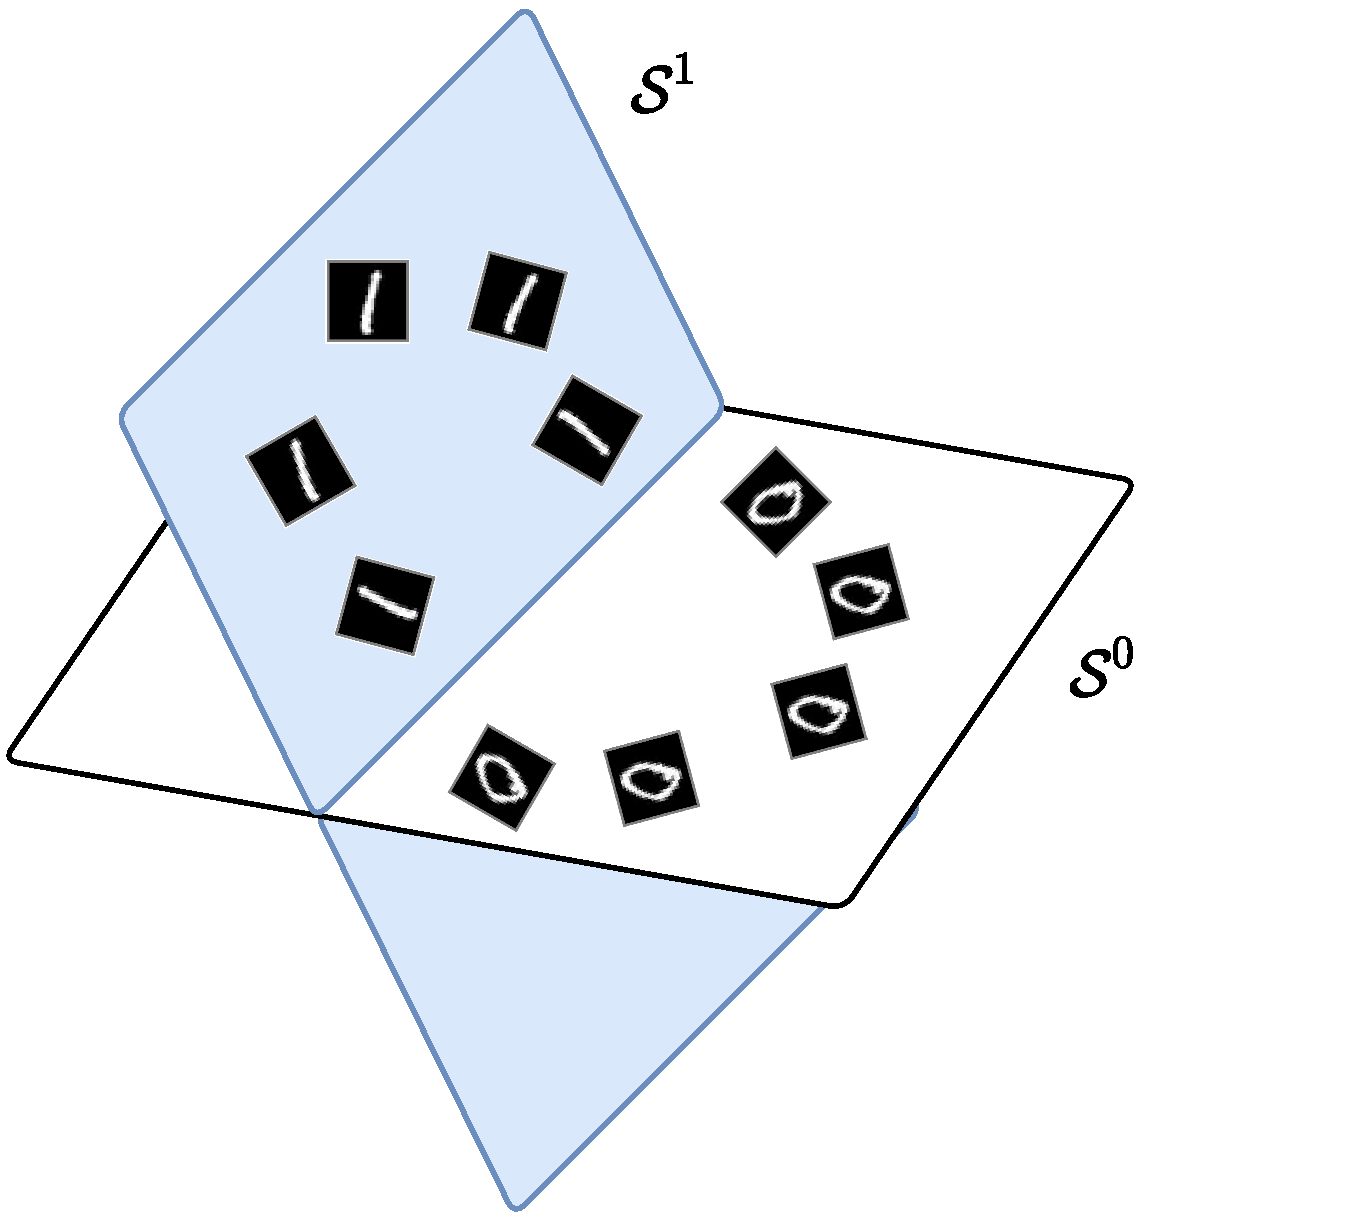
\includegraphics[width=\textwidth]{figs_chap4/ortho_diagram_1d.pdf}
    \end{subfigure}
    \hfill
    \begin{subfigure}[t]{0.4\textwidth}
        \centering
        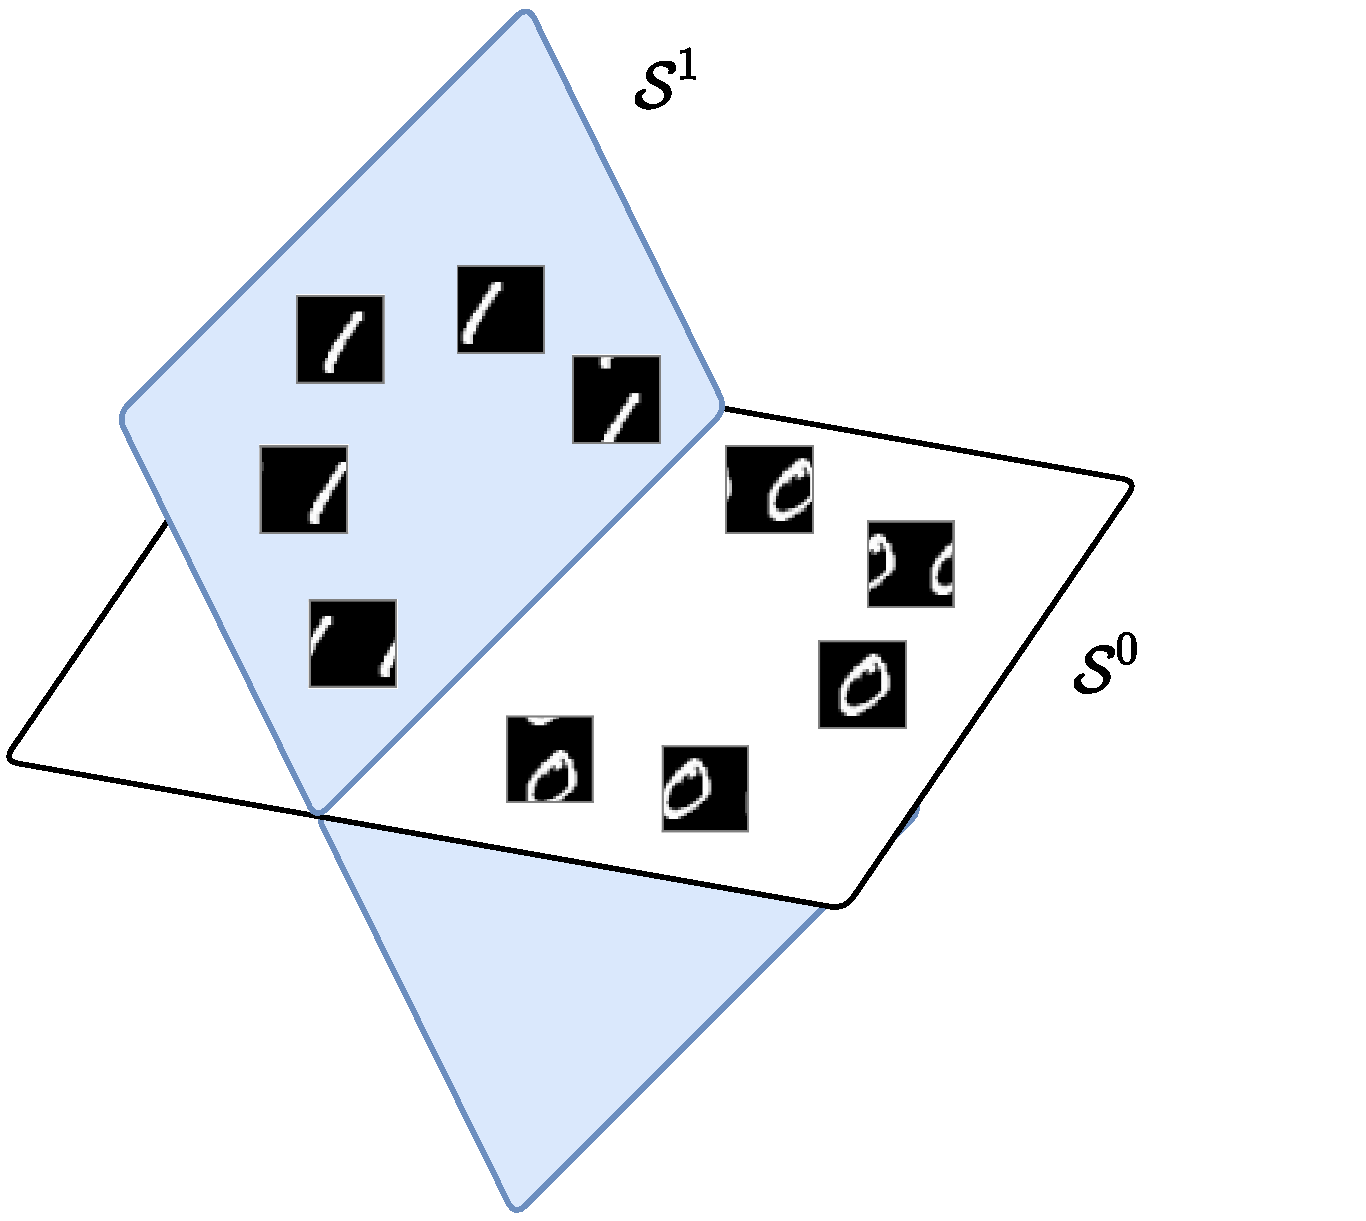
\includegraphics[width=\textwidth]{figs_chap4/ortho_diagram_2d.pdf}
    \end{subfigure}
    \caption{所寻求的对图像旋转(左)或平移(右)等变/不变的表示的图示:每个类别的所有变换后的图像都被映射到同一个子空间,该子空间与其他子空间不相干。嵌入在每个子空间中的特征对变换群是等变的,而每个子空间对这类变换是不变的。}\label{fig:ortho-invariance-diagram}
\end{figure}

\paragraph{一维序列数据与平移不变性} 为了对在平移下不变的一维数据 $\bm x = [x(0), x(1), \ldots, x(D-1)] \in \Re^D$ 进行分类,我们取 $\mathbb{G}$ 为所有循环平移的群。每个观测 $\bm x_i$ 生成一个平移副本族 $\{ \x_i \circ \mathfrak{g} \, | \, \mathfrak{g} \in \mathbb G \}$,它们是循环矩阵 $\circm(\bm x_i) \in \Re^{D \times D}$ 的列,由下式给出
\begin{equation}
\circm(\x) \,\doteq\, \left[ \begin{array}{ccccc} x(0) & x(D-1) & \dots & x(2) & x(1) \\ x(1) & x(0) & x(D-1) & \cdots & x(2) \\ \vdots & x(1) & x(0) &\ddots & \vdots \\ x(D-2) &  \vdots & \ddots & \ddots & x(D-1) \\ x(D-1) & x(D-2) & \dots & x(1) & x(0)   \end{array} \right]  \in \Re^{D \times D}.
\end{equation}
关于循环矩阵的性质,我们请读者参考 \cite{Kra2012OnCM}。为简单起见,令 $\bm Z^1 \doteq [ \z_{1}^1, \dots, \z_{N}^1 ] = \X \in \Re^{d \times N}$。\footnote{同样,为了简化讨论,我们暂时假设初始特征 $\Z^1$ 是 $\X$ 本身,因此具有相同的维度 $d$,即 $D=d$。但这并非必须如此,因为我们很快会看到我们需要将 $\X$ 提升到更高的维度。} 那么,如果我们从它们的循环族 $\circm(\bm Z^1) = \left[ \circm(\z_{1}^1), \dots, \circm(\z_{N}^1) \right] \in \Re^{d \times (dN)}$ 构建 ReduNet 会发生什么?也就是说,我们希望通过 ReduNet 将所有这些压缩并映射到同一个子空间。

请注意,现在的数据协方差矩阵:
\begin{eqnarray}
\circm(\bm Z^1) \circm(\bm Z^1)^\top
&=& \left[ \circm(\z_{1}^1), \dots, \circm(\z_{N}^1) \right] \left[ \circm(\z_{1}^1), \dots, \circm (\z_{N}^1) \right]^\top \nonumber \\
&=& \sum_{i =1}^N \circm(\z_{i}^1) \circm(\z_{i}^1)^\top \;\in \Re^{d\times d}
\end{eqnarray}
与这个样本族相关联的矩阵{\em 自动地}是一个(对称的)循环矩阵。此外,由于循环性质在求和、求逆和乘积下是保持的,矩阵 $\bm E^1$ 和 $\bm C^1_k$ 也自动是循环矩阵,它们对特征向量 $\bm z \in \Re^d$ 的应用可以用循环卷积“$\circledast$”来实现。
具体来说,我们有以下命题。

\begin{proposition}[$\bm E^1$ 和 $\bm C^1_k$ 的卷积结构]
矩阵
\begin{equation}
    \bm E^1 = \alpha\big(\bm I + \alpha \circm(\bm Z^1) \circm(\bm Z^1)^\top \big)^{-1}
\end{equation}
是一个循环矩阵,并表示一个循环卷积:
$$\bm E^1 \z = \bm e_1 \circledast \z,$$
其中 $\bm e_1 \in \Re^d$ 是 $\bm E^1$ 的第一列向量,“$\circledast$”是循环卷积,定义为
\begin{equation*}
    (\bm e_1 \circledast \bm z)_{i} \doteq \sum_{j=0}^{d-1} e_1(j) x(i+ d-j \,\, \textsf{mod} \,\,d).
\end{equation*}
类似地,与 $\bm Z^1$ 的任何子集相关的矩阵 $\bm C^1_k$ 也是循环卷积。
\label{prop:circular-conv-1}
\end{proposition}

不仅 ReduNet 的第一层参数 $\bm E^1$ 和 $\bm{C}^1_k$ 变成了循环卷积,而且下一层的特征也保持为循环矩阵。
也就是说,在 \eqref{eqn:layer-approximate} 中应用于 $\z^1 \in \Re^d$ 的所有平移版本的增量特征变换,由下式给出
\begin{equation}
    \circm(\z^1) + \eta \cdot \bm E^1 \circm(\z^1) - \eta \cdot \bm \sigma \Big([\bm{C}_1^1 \circm(\z^1), \ldots, \bm{C}^1_K \circm(\z^1)] \Big),
\end{equation}
是一个循环矩阵。这意味着不需要像第一层那样从第二层特征构建循环族。
通过记为
\begin{equation}
\z^{2} \propto \z^{1} +\eta \cdot g(\z^{1}, \bm \theta^{1}) =  \z^1 + \eta \cdot \bm e_{1} \circledast \z^{1} -  \eta \cdot \bm \sigma\Big([\bm{c}_{1}^{1} \circledast \z^{1}, \dots, \bm{c}^{1}_{K} \circledast \z^{1}]\Big),
\label{eqn:approximate-convolution}
\end{equation}
下一层的特征可以写成
$$\circm(\bm Z^2) = \big[ \circm( \bm z_{1}^1 + \eta g( \bm z_{1}^1, \bm \theta^1)), \dots, \circm( \bm z_{N}^1 + \eta g(\bm z_{N}^1, \bm \theta^1)) \big].$$
通过归纳法继续,我们看到所有基于 $\circm(\bm Z^\ell)$ 的矩阵 $\bm E^\ell$ 和 $\bm C^\ell_k$ 都是循环的,所有特征也是如此。
凭借数据的这些性质,ReduNet 已经呈现出卷积网络的形式,{\em 无需显式选择这种结构!}

\paragraph{不变性与稀疏性之间的基本权衡。}
不过有一个问题:通常情况下,一个向量 $\z$ 的所有循环排列集合会给出一个满秩矩阵。也就是说,与每个样本(因此每个类别)相关联的 $d$ 个“增强”特征通常已经张成了整个空间 $\Re^d$。例如,一个 delta 函数 $\delta(d)$ 的所有平移版本可以生成任何其他信号,作为它们的(稠密的)加权叠加。MCR$^2$ 目标 \eqref{eqn:maximal-rate-reduction} 将无法区分不同类别的子空间。

一个自然的补救方法是通过将原始信号“提升”到更高维空间来提高数据的可分性,例如,通过获取它们对多个滤波器 $\bm k_1, \ldots, \bm k_C \in \Re^d$ 的响应:
\begin{equation}
\bm z[c] = \bm k_c \circledast \bm x  =  \circm(\bm k_c) \bm x \in \Re^d, \quad c = 1, \ldots, C.
\label{eqn:lift-1d}
\end{equation}
这些滤波器可以是预先设计的促进不变性的滤波器,\footnote{对于像音频这样的一维信号,可以考虑传统的短时傅里叶变换(STFT);对于二维图像,可以考虑二维小波,如 ScatteringNet \cite{scattering-net}。} 或者是从数据中自适应学习的,\footnote{对于学习的滤波器,可以像 PCANet \cite{chan2015pcanet} 中那样学习滤波器作为样本的主成分,或者从卷积字典学习 \cite{li2019multichannel,qu2019nonconvex} 中学习。} 或者像我们在实验中那样随机选择。这个操作将每个原始信号 $\x \in \Re^d$ 提升为一个 $C$ 通道的特征,记为 $\bar{\z}  \doteq [\z[1], \ldots, \z[C]]^\top \in \Re^{C\times d}$。
然后,我们可以在 $\bar{\z}$ 的向量表示上构建 ReduNet,记为
$\vec(\bar\z) \doteq [\z[1]^\top, \ldots, \z[C]^\top] \in \Re^{dC}$。
其所有平移版本的相关循环版本 $ \circm(\bar{\z})$ 及其数据协方差矩阵,记为 $\bar{\bm \Sigma}(\bar\z)$,由下式给出:
\begin{equation}
\begin{aligned}
 \circm(\bar{\z}) \doteq \left[\begin{matrix}
    \circm(\z[1])  \\ \vdots \\ \circm(\z[C]) \end{matrix} \right] \in \Re^{dC\times d},
    \quad  \bar{\bm \Sigma}(\bar\z) \doteq
    \left[\begin{matrix}
    \circm(\z[1]) \\ \vdots \\ \circm(\z[C]) \end{matrix} \right]
    \left[\begin{matrix}\circm(\z[1])^\top,\ldots, \circm(\z[C])^\top\end{matrix} \right] \in \Re^{dC\times dC},
    \label{eqn:W-multichannel}
\end{aligned}
\end{equation}
其中 $\circm(\z[c]) \in \Re^{d\times d}$ 且 $c \in [C]$ 是特征 $\bar \z$ 的第 $c$ 个通道的循环版本。那么 $\circm(\bar\z)$ 的列将最多张成 $\Re^{dC}$ 中一个 $d$ 维的真子空间。然而,这个简单的提升操作(如果是线性的)还不足以使类别可分——与其他类别相关的特征将张成{\em 相同}的 $d$ 维子空间。这反映了不变性与线性(子空间)建模之间的根本冲突:{\em 不能指望任意平移和叠加的信号属于同一个类别。}

\begin{figure}[t]
	\centerline{
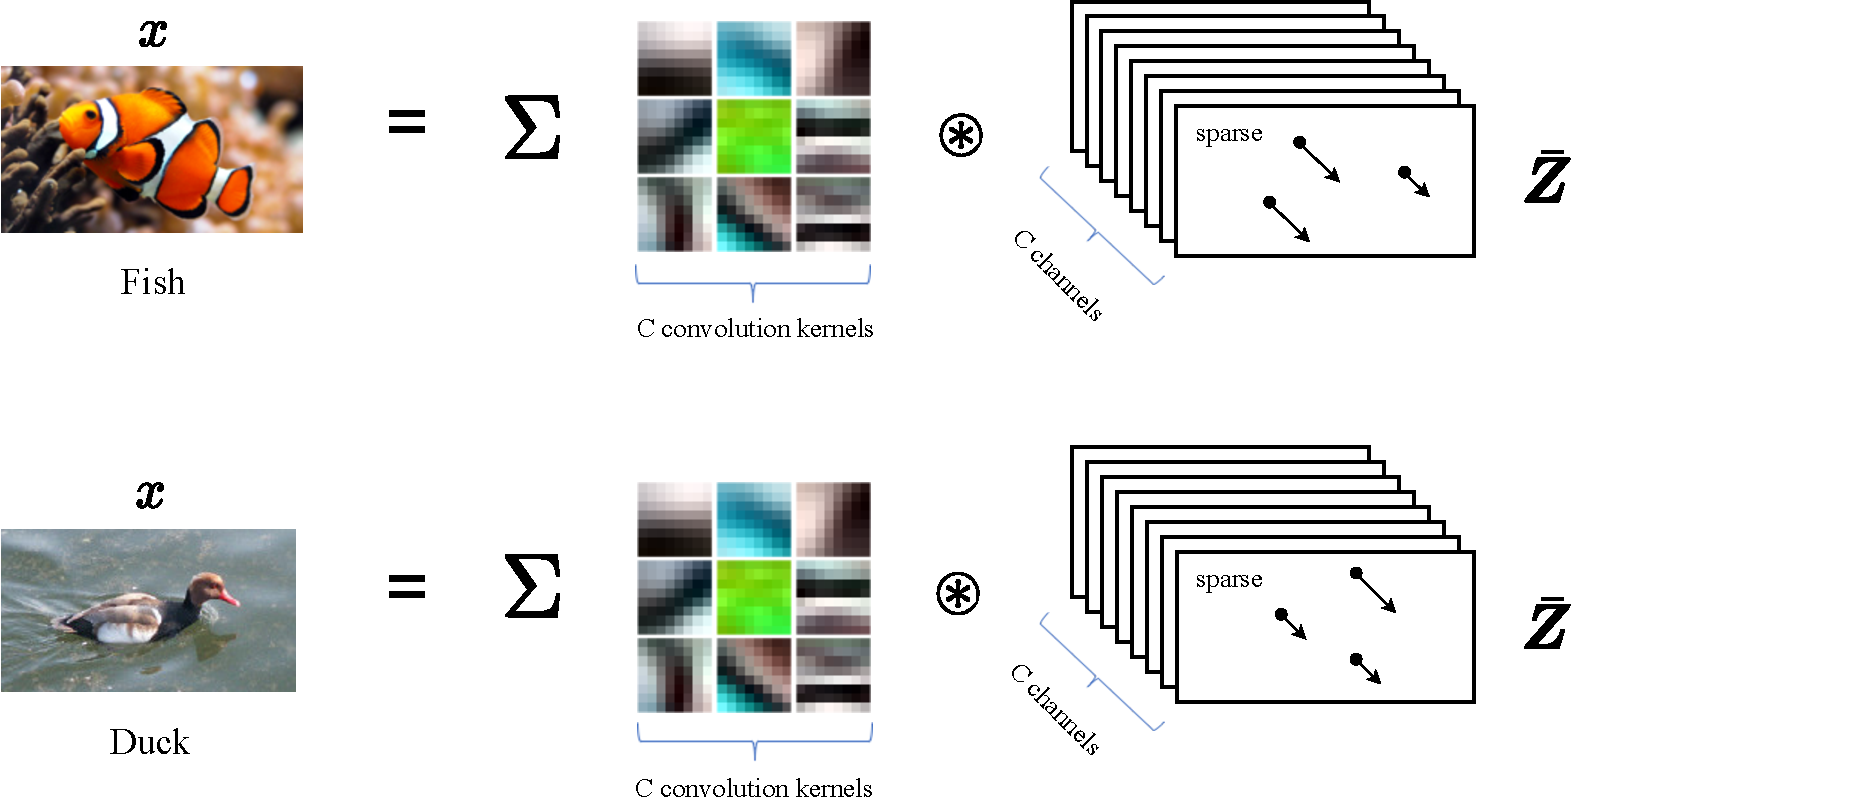
\includegraphics[width=0.9\textwidth]{figs_chap4/sparse-representation.pdf}}
	\caption{每个输入信号 $\bm x$(这里是一张图片)可以表示为与字典 $\bm D$ 中多个核 $\bm d_c$ 进行稀疏卷积的叠加。}
	\label{fig:multi-channel-sparse-representation}
\end{figure}
解决这个冲突的一种方法是利用每个类别内部的额外结构,即{\em 稀疏性}:每个类别内的信号不是由一些基础原子(或基元)的任意线性叠加生成的,而只是它们及其平移版本的{\em 稀疏}组合,如图 \ref{fig:multi-channel-sparse-representation} 所示。更精确地说,让 $\bm D_k = [\bm d_{k,1}, \ldots, \bm d_{k,c}]$ 表示一个包含与类别 $k$ 相关的一组原子的矩阵,也称为字典,那么这个类别中的每个信号 $\x$ 都是稀疏生成的:
\begin{equation}
    \x = \bm d_{k,1} \circledast z_1 + \ldots + \bm d_{k,c} \circledast z_c = \circm(\bm{D}_k)\z,
\end{equation}
对于某个稀疏向量 $\z$。不同类别中的信号则由不同的字典生成,这些字典的原子(或基元)彼此不相干。由于不相干性,一个类别中的信号不太可能被任何其他类别中的原子稀疏地表示。因此,所有信号都可以表示为
\begin{equation}
\x = \big[\circm(\bm{D}_1), \circm(\bm{D}_2), \ldots, \circm(\bm{D}_K)\big] \bar \z,
\end{equation}
其中 $\bar \z$ 是稀疏的。\footnote{请注意,类似地稀疏表示模型早已被提出并用于分类目的,例如在人脸识别等应用中,展示了出色的效果 \cite{Wright:2009,wagner2012toward}。最近,\cite{papyan2017convolutional} 提出了卷积稀疏编码模型,作为解释深度卷积网络结构的框架。} 关于如何从样本数据中学习最紧凑和最优的稀疏化字典,有大量的文献,例如 \cite{li2019multichannel,qu2019nonconvex},以及随后如何解决逆问题并计算相关的稀疏码 $\z$ 或 $\bar \z$。最近 \cite{qu2020nonconvex,Qu2020Geometric} 的研究甚至表明,在广泛的条件下,卷积字典学习问题可以被有效且高效地解决。

然而,对于分类等任务,我们不一定对精确的最优字典或每个信号的精确稀疏码感兴趣。我们主要关心的是,每个类别的稀疏码集合是否能与其他类别的稀疏码充分分离。在稀疏生成模型的假设下,如果卷积核 $\{\bm k_c\}_{c=1}^C$ 与上述稀疏化字典 $\bm D = [\bm D_1, \ldots, \bm D_K]$ 的“转置”或“逆”(也称为{\em 分析滤波器} \cite{Cosparse-Nam,Analysis-Filter})匹配得很好,那么一个类别中的信号将只对这些滤波器的一小部分有高响应,而对其他滤波器有低响应(由于不相干性假设)。然而,在实践中,通常足够大量的(比如说 $C$ 个)随机滤波器 $\{\bm k_c\}_{c=1}^C$ 就足以确保提取的 $C$ 通道特征
\begin{equation}
\big[\bm k_1 \circledast \x, \bm k_2 \circledast \x, \ldots, \bm k_C \circledast \x\big]^\top = \big[\circm(\bm k_1) \x, \ldots, \circm(\bm k_C) \x \big]^\top \in \Re^{C\times d}
\end{equation}
对于不同类别具有不同的滤波器响应模式,从而使不同类别可分 \cite{chan2015pcanet}。

因此,在我们的框架中,通道数(或网络宽度)在很大程度上扮演着{\em 统计资源}的角色,而层数(网络深度)则扮演着{\em 计算资源}的角色。压缩感知理论精确地描述了需要多少测量才能保留数据的内在低维结构(包括可分性)\cite{Wright-Ma-2021}。% 由于最优稀疏编码不是本文的重点,我们将在实验中使用简单的随机滤波器设计,这足以验证概念。尽管更好的学习或设计的稀疏化字典和稀疏编码方案肯定会带来更好的分类性能,但计算成本也更高。

\begin{figure}[t]
	\centerline{
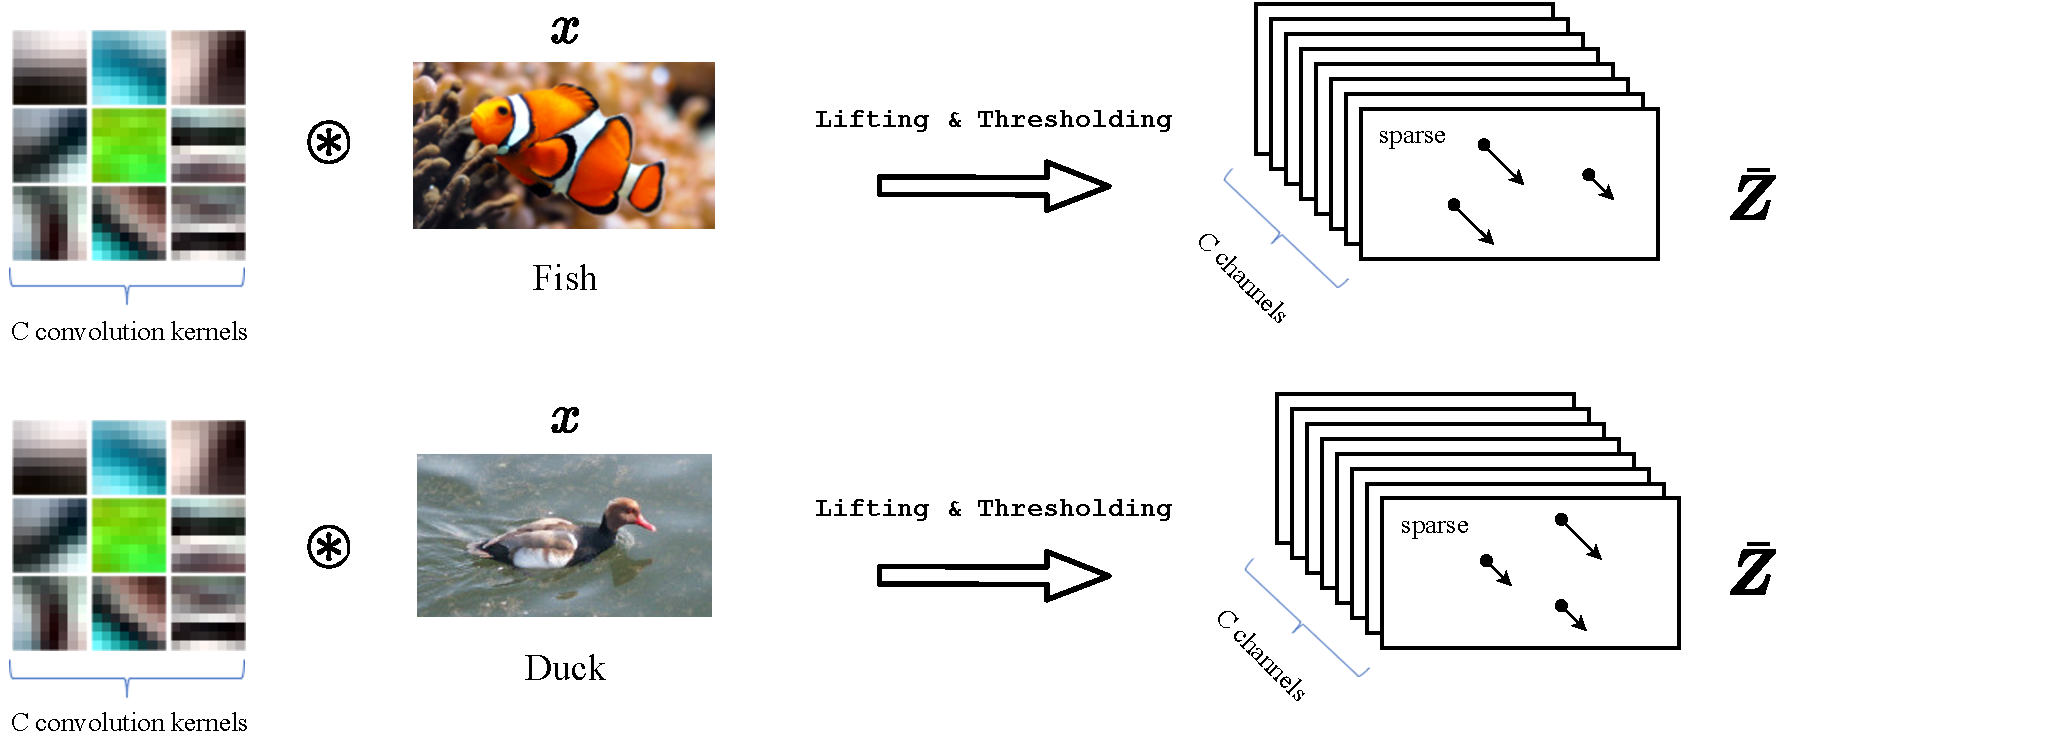
\includegraphics[width=0.95\textwidth]{figs_chap4/sparse-lifting.pdf}}
\caption{通过与多个核 $\bm k_c$ 进行卷积然后进行稀疏化,来估计输入信号 $\bm x$(这里是一张图片)的稀疏码 $\bar{\bm z}$。}
		\label{fig:multi-channel-sparse-lifting}
\end{figure}
多通道响应 $\bar \z$ 应该是稀疏的。因此,为了近似稀疏码 $\bar \z$,我们可以在上述滤波器输出上进行逐项的{\em 促进稀疏性的非线性阈值处理},比如 $\bm \tau(\cdot)$,将低响应(例如绝对值低于 $\epsilon$)或负响应设为零:
\begin{equation}
\bar \z \doteq \bm \tau \left( \big[\circm(\bm k_1) \x, \ldots, \circm(\bm k_C) \x \big]^\top \right) \in \Re^{C \times d}.
\label{eqn:sparse-lifting}
\end{equation}
图 \ref{fig:multi-channel-sparse-lifting} 说明了基本思想。关于稀疏化阈值算子的设计,可以参考 \cite{Analysis-Filter} 进行更系统的研究。然而,这里我们不那么关心获得最佳的稀疏码,只要这些码足够可分即可。因此,非线性算子 $\bm \tau$ 可以简单地选择为软阈值或 ReLU。
这些假定为稀疏的特征 $\bar \z$ 可以被假设位于 $\mathbb{R}^{dC}$ 的一个低维(非线性)子流形上,这个子流形可以通过后续的 ReduNet 层进行线性化并与其他类别分离,稍后在图 \ref{fig:learn-to-classify-diagram} 中会进行说明。

从这些多通道特征 $\bar\Z \doteq [\bar \z_1, \ldots, \bar \z_N] \in \Re^{C \times d \times N}$ 的循环版本,即 $\circm(\bar\Z) \doteq [ \circm(\bar\z_1), \dots, \circm(\bar\z_N)] \in \Re^{dC \times dN}$ 构建的 ReduNet,保留了上述良好的不变性性质:线性算子,现在记为 $\bar{\bm E}$ 和 $\bar{\bm C}_k$,仍然是块循环的,并表示{\em 多通道一维循环卷积。}
具体来说,我们有以下结果。
\begin{proposition}[$\bar{\bm E}$ 和 $\bar{\bm C}_k$ 的多通道卷积结构]
矩阵
\begin{equation}
\label{eq:def-E-bar}
\bar{\bm E} \doteq \alpha\left(\bm I + \alpha\, \circm(\bar\Z) \circm(\bar\Z)^\top \right) ^{-1}
\end{equation}
是块循环的,即
\begin{equation*}
    \bar{\bm E} =
    \left[\begin{matrix}
        \bar{\bm E}_{1, 1} & \cdots & \bar{\bm E}_{1, C}\\
        \vdots & \ddots & \vdots \\
        \bar{\bm E}_{C, 1} & \cdots & \bar{\bm E}_{C, C}\\
    \end{matrix}\right] \in \Re^{dC \times dC},
\end{equation*}
其中每个 $\bar{\bm E}_{c, c'}\in \Re^{d \times d}$ 是一个循环矩阵。此外,$\bar{\bm E}$ 表示一个多通道循环卷积,即对于任何多通道信号 $\bar\z \in \Re^{C \times n}$,我们有
$$\bar{\bm E} \cdot \textsf{vec}(\bar\z) = \textsf{vec}( \bar{\bm e} \circledast \bar\z).$$
在上述公式中,$\bar{\bm e} \in \Re^{C \times C \times d}$ 是一个多通道卷积核,其中 $\bar{\bm e}[c, c'] \in \Re^{d}$ 是 $\bar{\bm E}_{c, c'}$ 的第一列向量,而 $\bar{\bm e} \circledast \bar\z \in \Re^{C \times d}$ 是多通道循环卷积,定义为
\begin{equation*}
    (\bar{\bm e} \circledast \bar\z)[c] \doteq \sum_{c'=1}^C \bar{\bm e}[c, c'] \circledast \bar{\z}[c'], \quad \forall c = 1, \ldots, C.
\end{equation*}
类似地,与 $\bar{\bm Z}$ 的任何子集相关的矩阵 $\bar{\bm C}_k$ 也是多通道循环卷积。
\label{prop:multichannel-circular-conv-1}
\end{proposition}
从命题 \ref{prop:multichannel-circular-conv-1} 可知,平移不变的 ReduNet 通过构造就是一个用于多通道一维信号的深度卷积网络。请注意,即使初始的提升核是分离的 \eqref{eqn:sparse-lifting},计算 $\bar{\bm E}$($\bar{\bm C_k}$ 也类似)时 \eqref{eq:def-E-bar} 中的矩阵求逆也会在所有 $C$ 个通道之间引入“串扰”。% 这种多通道混合效应在我们下面展示如何在频域中高效计算 $\bar{\bm E}$ 和 $\bar{\bm C}^j$ 时会变得更加清晰。
因此,这些多通道卷积通常是{\em 不可}深度分离的,不像 Xception 网络~\cite{Xception} 那样,后者曾被建议用于简化多通道卷积神经网络。\footnote{数据上的何种附加结构会导致深度可分离卷积仍然是一个开放问题。}

\begin{remark}[在频域中降低计算复杂性]
在 \eqref{eq:def-E-bar} 中计算 $\bar{\bm E}$ 需要对一个大小为 $dC \times dC$ 的矩阵求逆,其复杂度通常为 $O(d^3C^3)$。然而,通过利用循环矩阵可以被离散傅里叶变换(DFT)矩阵对角化的事实,可以显著降低复杂度。如 \cite{chan2021redunet} 所示,为了计算 $\bar{\bm E}$ 和 $\bar{\bm C}_k \in \Re^{dC \times dC}$,我们只需要在频域中计算 $d$ 次 $C\times C$ 块的逆,因此总复杂度变为 $O(dC^3)$。

\end{remark}

% \paragraph{频域中的快速计算。}



\paragraph{整体网络架构与比较。}
根据上述推导,我们看到,为了找到一个对平移不变的多类信号/图像的线性判别表示(LDR),稀疏编码、多层架构、多通道卷积、不同的非线性激活以及频谱计算都成为有效和高效实现该目标的{\em 必要}组成部分。图 \ref{fig:learn-to-classify-diagram} 说明了通过对输入稀疏码进行不变率缩减来学习这种表示的整个过程。

\begin{figure}[t]
    \centering
    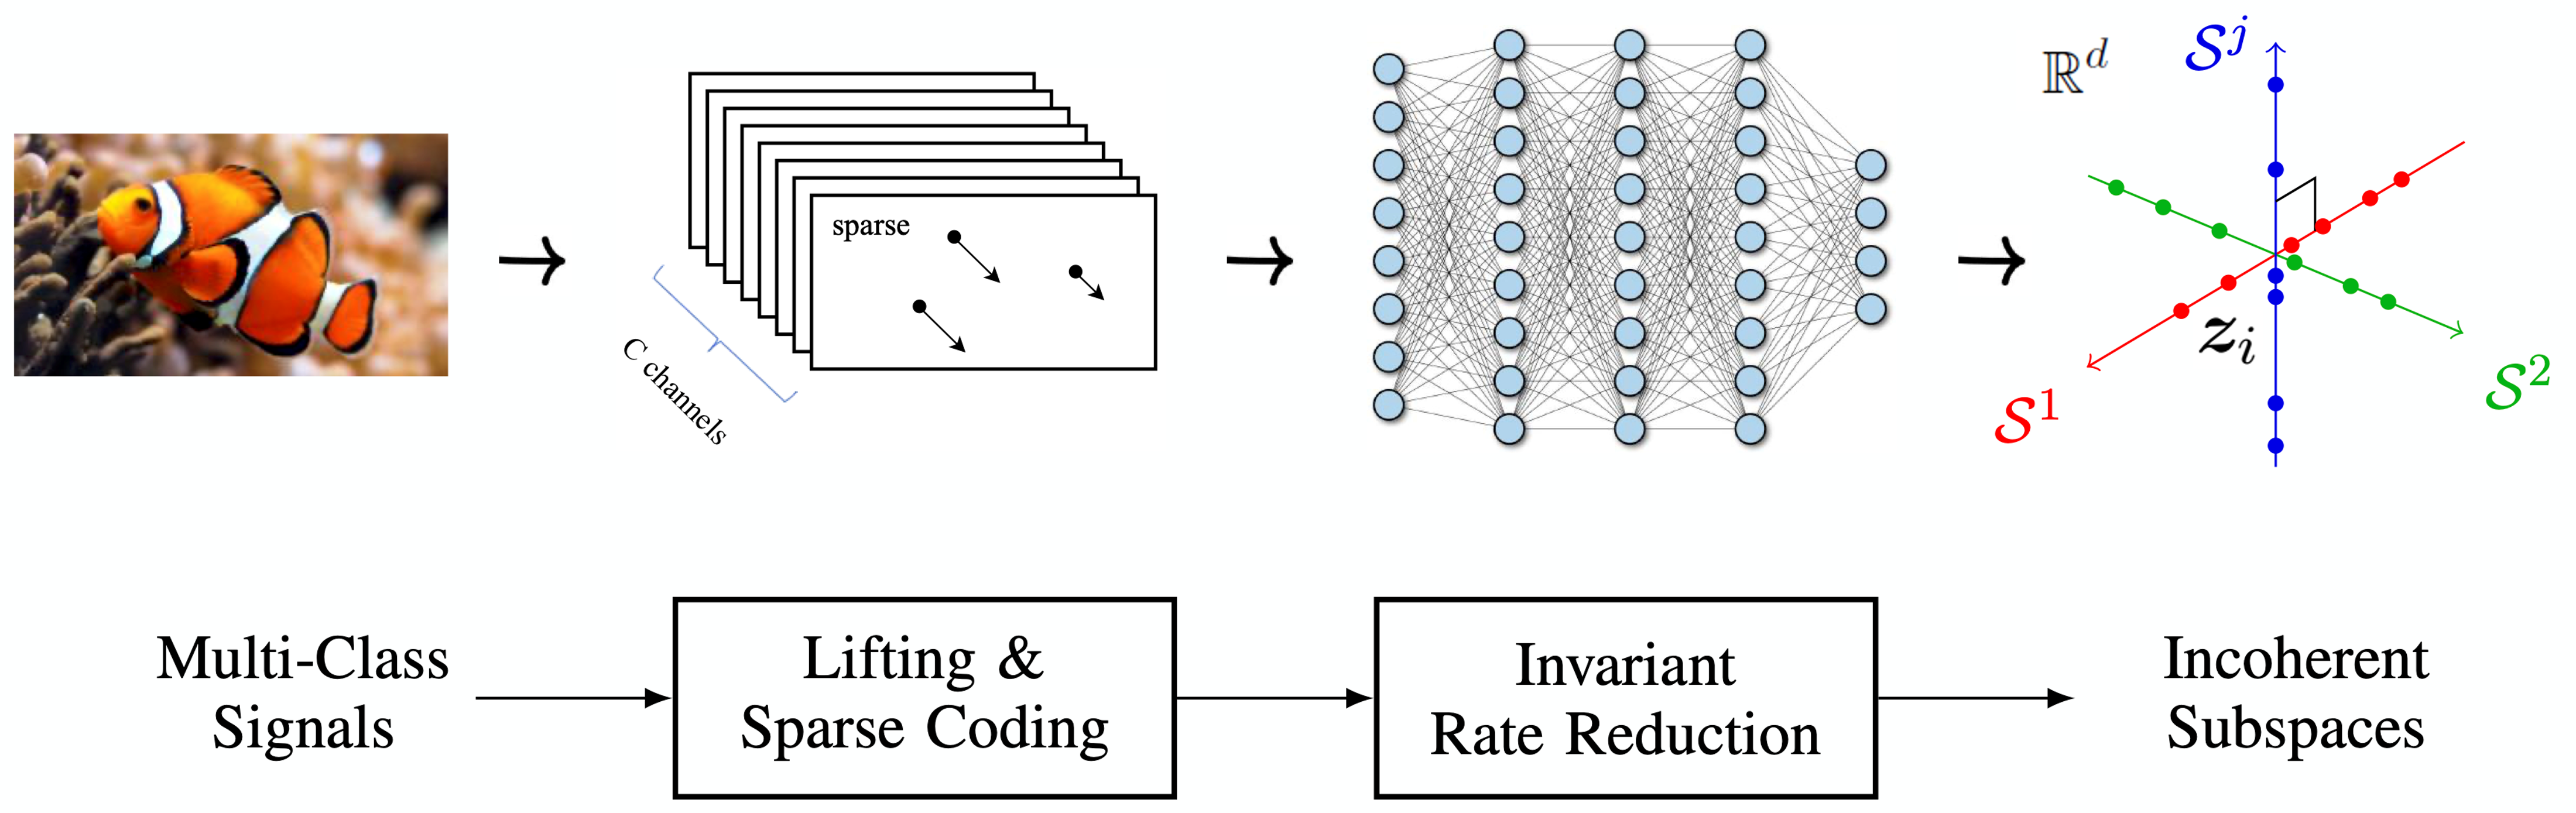
\includegraphics[width=0.98\linewidth]{figs_chap4/learn_to_classify_diagram_updated.png}
    \caption{具有平移不变性的多类信号分类的整个过程:多通道提升、稀疏编码,然后是一个用于不变率缩减的多通道卷积 ReduNet。这些组件是{\em 必要的},以便将平移不变的多类信号映射到不相干的(线性)子空间作为 LDR。请注意,大多数现代深度神经网络的架构都与此过程相似。如此学习到的 LDR 有助于后续任务,如分类。}
    \label{fig:learn-to-classify-diagram}
\end{figure}

%\yima{一些简单的例子,就像我们在论文中用数字做的实验一样?例子对于教学很重要!} \yaodong{在下面添加了图和段落。}

\begin{example}[数字的不变分类]
接下来,我们提供 ReduNet 在真实 10 类 MNIST 数据集上学习\textit{旋转}不变特征的经验性能。
我们在图像 $\bm{x}\in\mathbb{R}^{H\times W}$ 上施加一个极坐标网格,其几何中心是二维极坐标网格的中心(如图 \ref{fig:samples-invariant-1d-mnist-diagram} 所示)。
对于每个半径 $r_i$, $i \in [C]$,我们可以相对于每个角度 $\gamma_l =l\cdot({2\pi}/\Gamma)$(其中 $l \in [\Gamma]$)采样 $\Gamma$ 个像素。
然后,给定一个来自数据集的样本图像 $\bm{x}$,我们用一个多通道信号 $\bm{x}_p \in\R^{\Gamma\times C}$ 来表示该图像在(采样的)极坐标中的形式。
这里的目标是学习一个旋转不变的表示,即我们期望学习 $f(\cdot, \bm{\theta})$ 使得 $\{f(\bm{x}_p \circ \mathfrak{g}, \bm{\theta})\}_{\mathfrak{g} \in\mathbb{G}}$ 位于同一个子空间中,其中 $\mathfrak{g}$ 是极角上的循环平移。
我们使用 $N=100$ 个训练样本(每个类别 10 个),并设置 $\Gamma=200, C=15$ 进行极坐标采样。
通过在极坐标中执行上述采样,我们可以得到数据矩阵 $\bm{X}_p \in \mathbb{R}^{(\Gamma\cdot C) \times N}$。
对于 ReduNet,我们设置层数/迭代次数 $L=40$,精度 $\epsilon=0.1$,步长 $\eta=0.5$。在第一层之前,我们用 20 个大小为 5 的随机高斯核进行一维循环卷积来提升输入。

\begin{figure}[t]
    \begin{subfigure}[t]{0.3\textwidth}
        \centering
        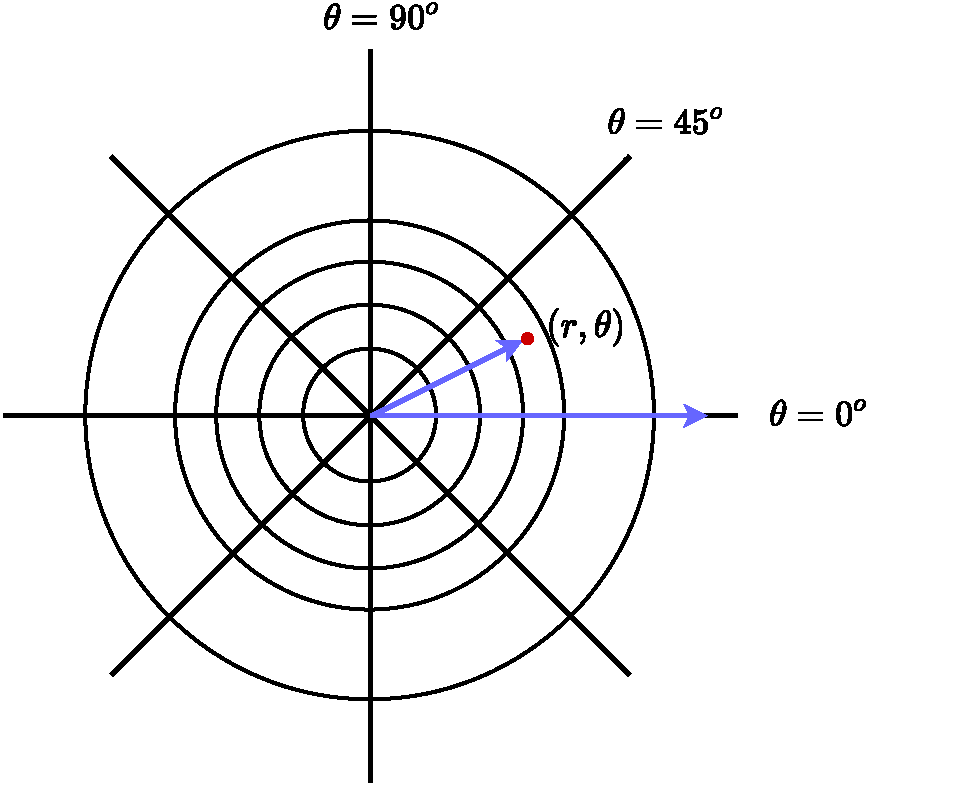
\includegraphics[width=\textwidth]{figs_chap4/1d-rotation.pdf}
        \caption{$\bm{X}_{\text{rotation}}$}
    \end{subfigure}
    \hfill
    \begin{subfigure}[t]{0.3\textwidth}
        \centering
        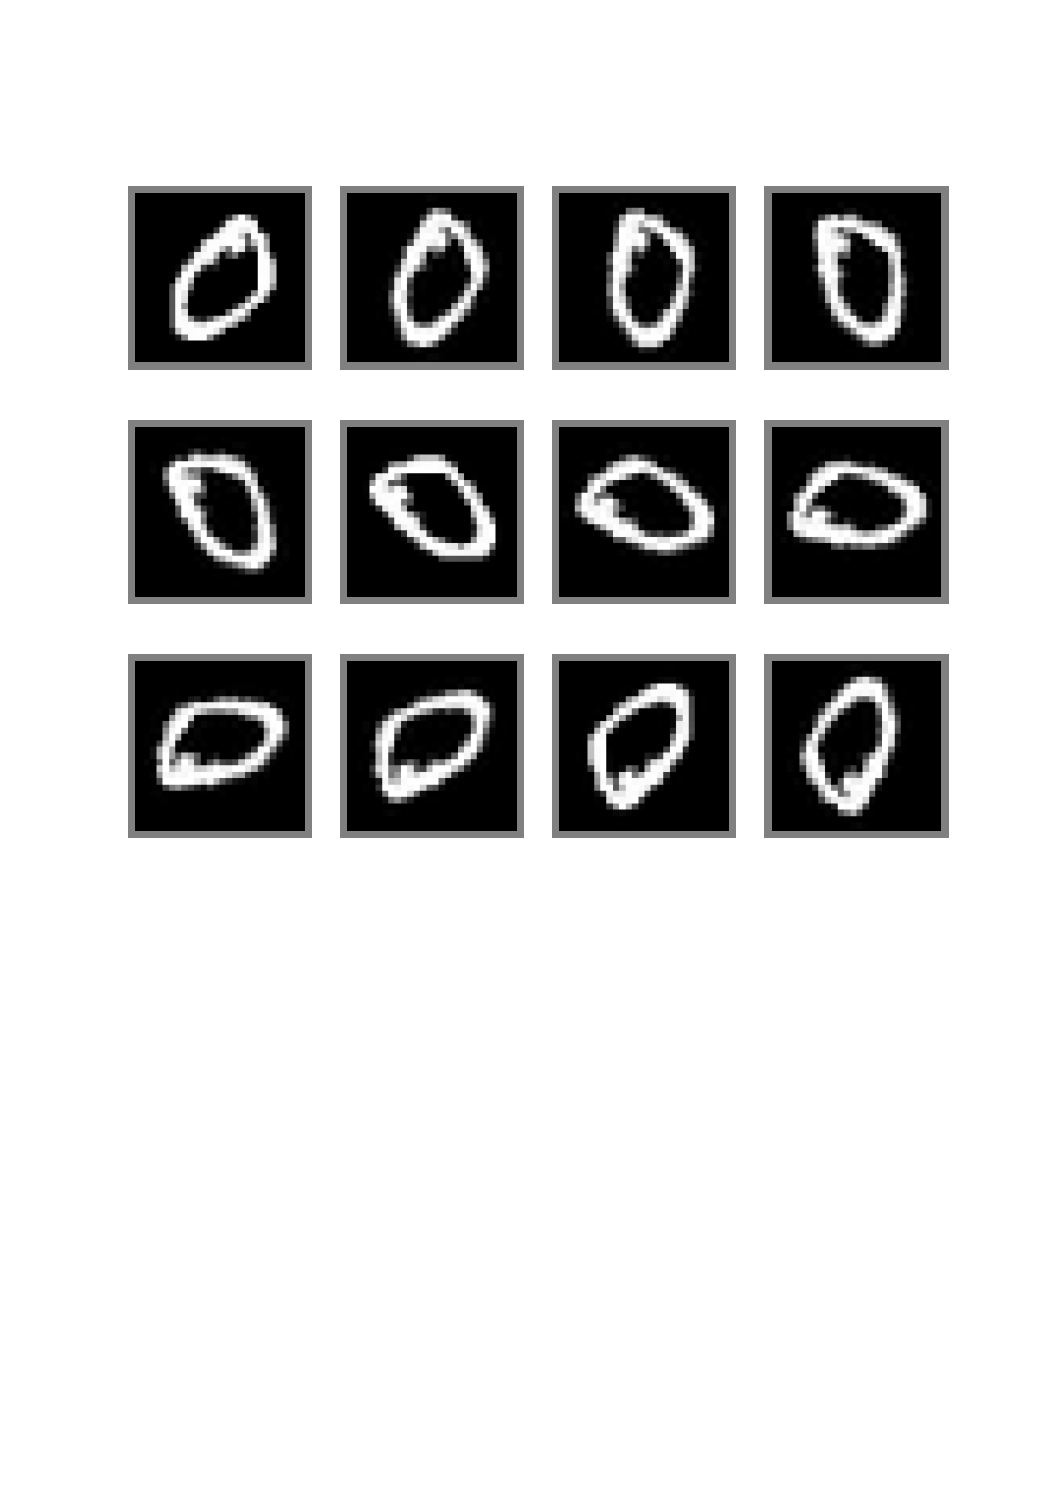
\includegraphics[width=\textwidth]{figs_chap4/mnist1d_img0.pdf}
        \caption{$\bm{Z}_{\text{rotation}}$}
    \end{subfigure}
    \hfill
    \begin{subfigure}[t]{0.3\textwidth}
        \centering
        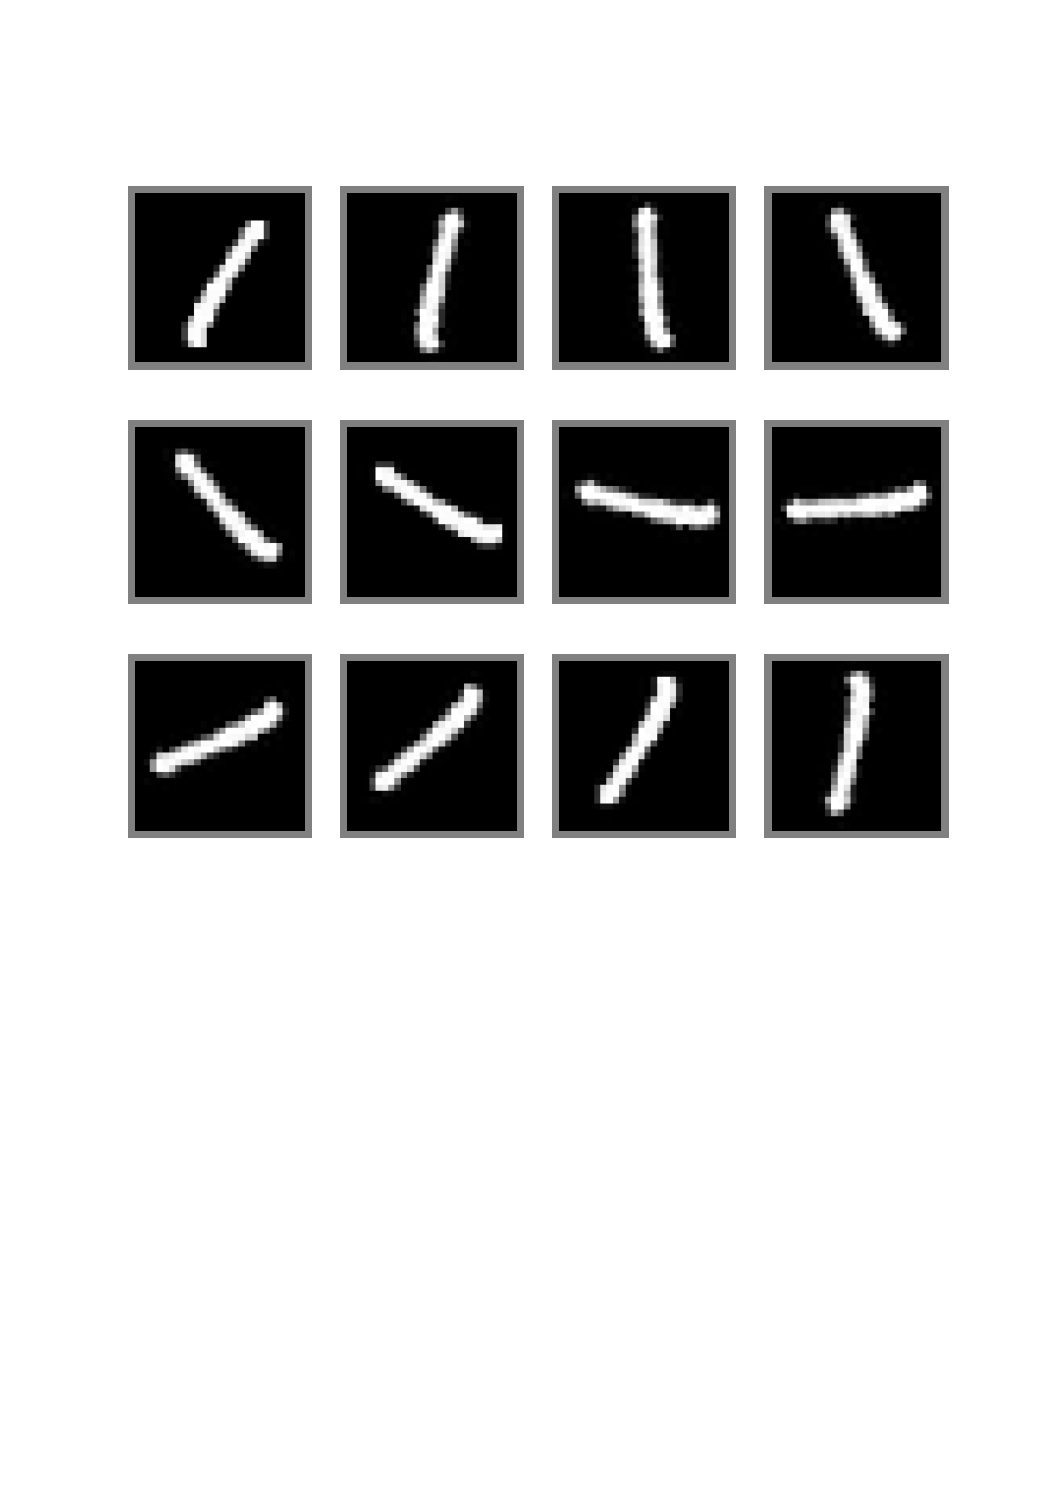
\includegraphics[width=\textwidth]{figs_chap4/mnist1d_img1.pdf}
        \caption{损失}
    \end{subfigure}
    \caption{\small MNIST 数字旋转图像的示例,每个旋转 18$^{\circ}$。(\textbf{左})极坐标表示示意图;(\textbf{右})数字‘0’和‘1’的旋转图像。}
    \label{fig:samples-invariant-1d-mnist-diagram}
\end{figure}


为了评估学习到的表示,每个训练样本都通过其 20 个旋转版本进行增强,每个版本以步长=10 进行平移。我们计算了 $m \times 20$ 个增强训练输入 $\bm{X}_{\text{rotation}}$ 之间的余弦相似度,结果如图 \ref{fig:redu-invariant-1d-mnist-diagram} (\textbf{a}) 所示。
我们比较了所有增强版本的学习特征之间的余弦相似度,即 $\bar{\bm{Z}}_{\text{rotation}}$,并将结果总结在图 \ref{fig:redu-invariant-1d-mnist-diagram} (\textbf{b}) 中。
正如我们所见,如此构建的旋转不变 ReduNet 能够将来自 10 个不同类别的训练数据(以及其所有旋转版本)映射到 10 个几乎正交的子空间中。也就是说,学习到的子空间对极角上的平移变换是真正不变的。接下来,我们随机抽取另外 100 个测试样本,并遵循相同的增强程序。
在图 \ref{fig:redu-invariant-1d-mnist-diagram} (\textbf{c}) 中,我们可视化了 ReduNet 在训练和测试数据集上第 $\ell$ 层表示的 MCR$^{2}$ 损失。从这些结果中,我们可以发现构建的 ReduNet 确实能够最大化 MCR$^{2}$ 损失,并能很好地泛化到测试数据。



\begin{figure}[t]
    \begin{subfigure}[t]{0.3\textwidth}
        \centering
        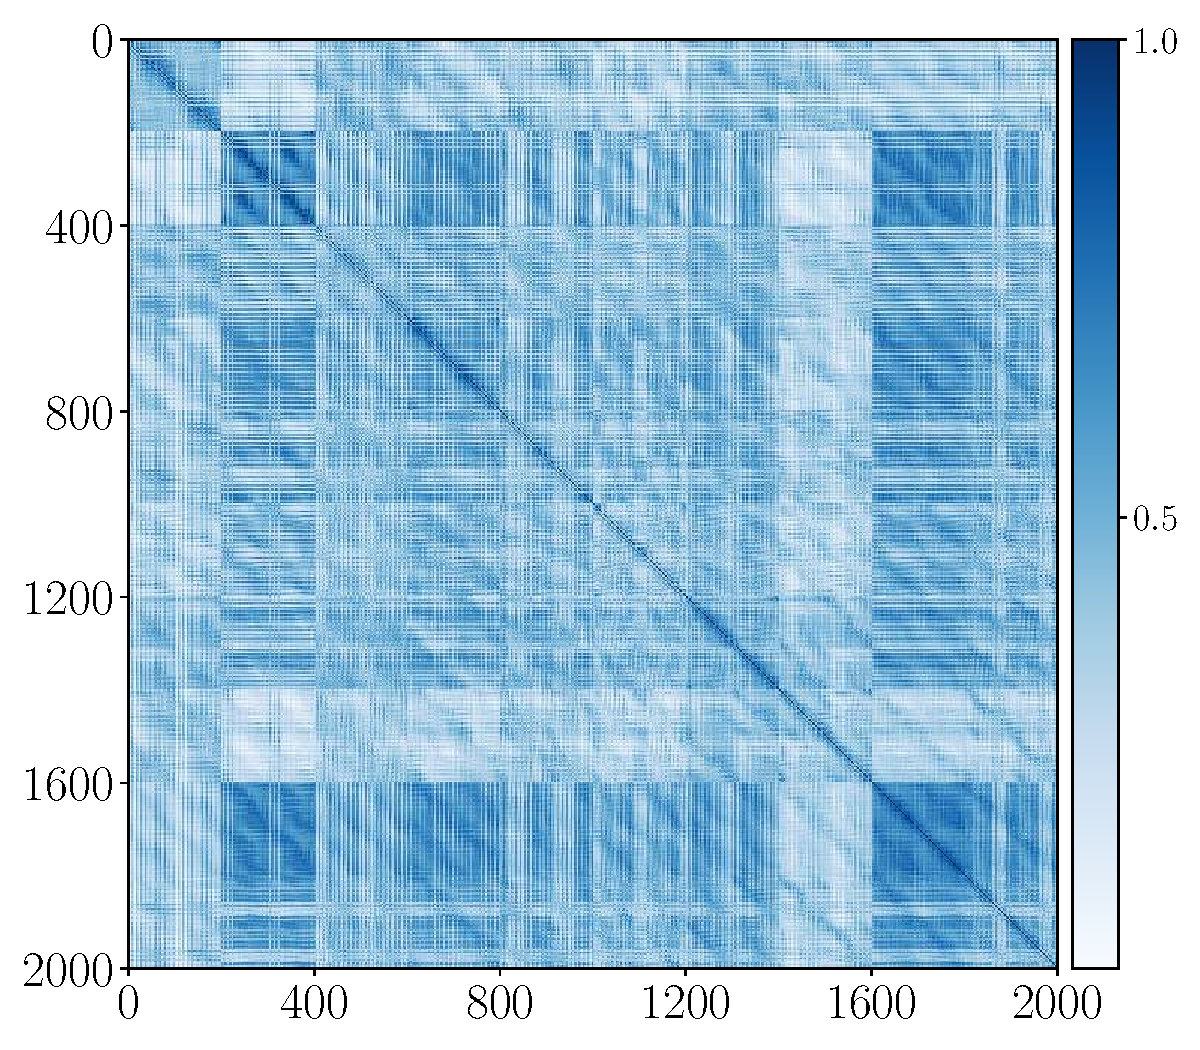
\includegraphics[width=\textwidth]{figs_chap4/mnist1d-heatmap-X_translate_train_all.pdf}
        \caption{$\bm{X}_{\text{rotation}}$}
    \end{subfigure}
    \hfill
    \begin{subfigure}[t]{0.3\textwidth}
        \centering
        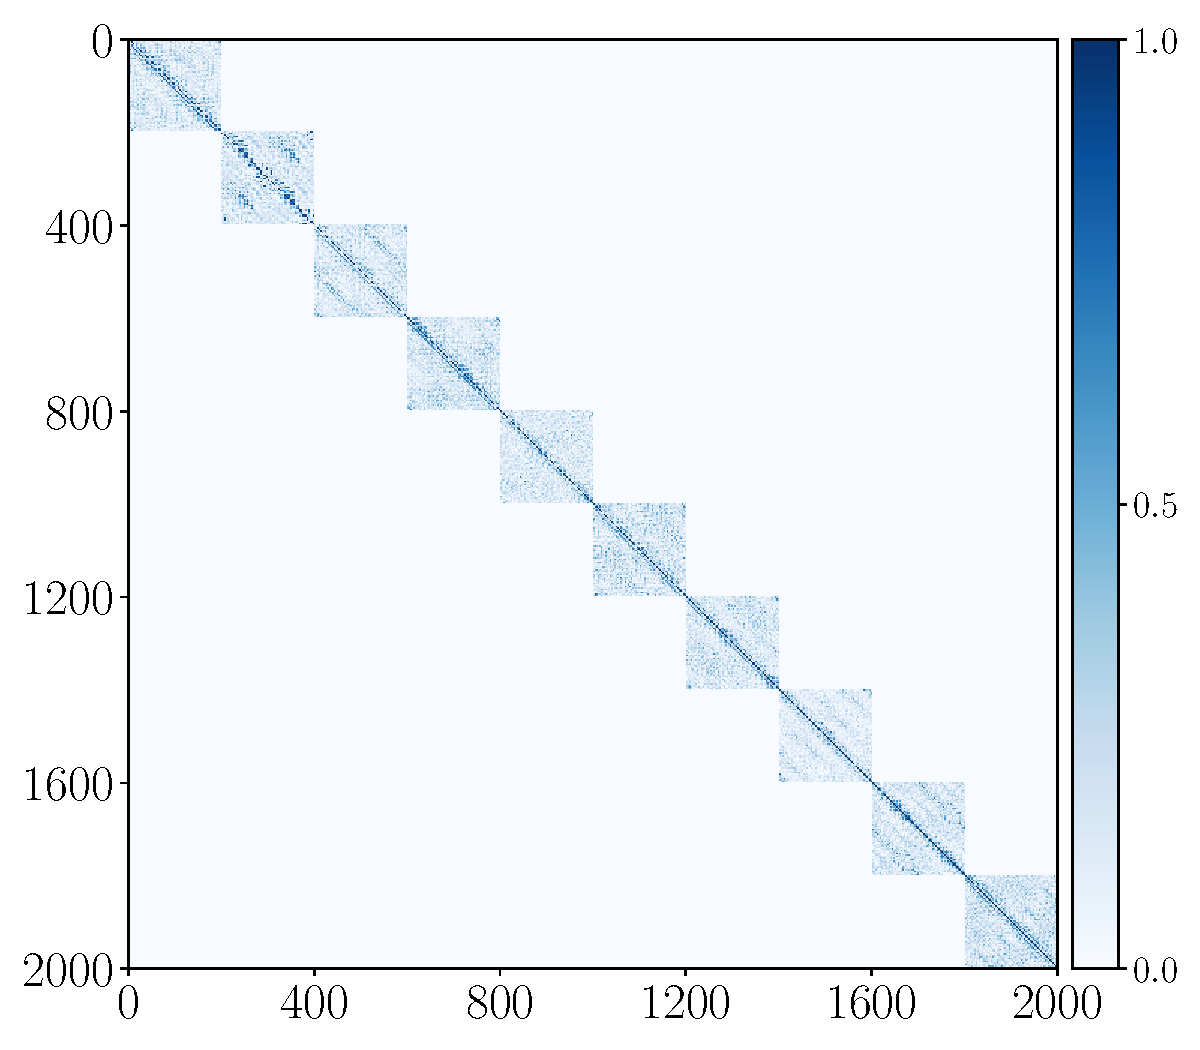
\includegraphics[width=\textwidth]{figs_chap4/mnist1d-heatmap-Z_translate_train_all.pdf}
        \caption{$\bm{Z}_{\text{rotation}}$}
    \end{subfigure}
    \hfill
    \begin{subfigure}[t]{0.32\textwidth}
        \centering
        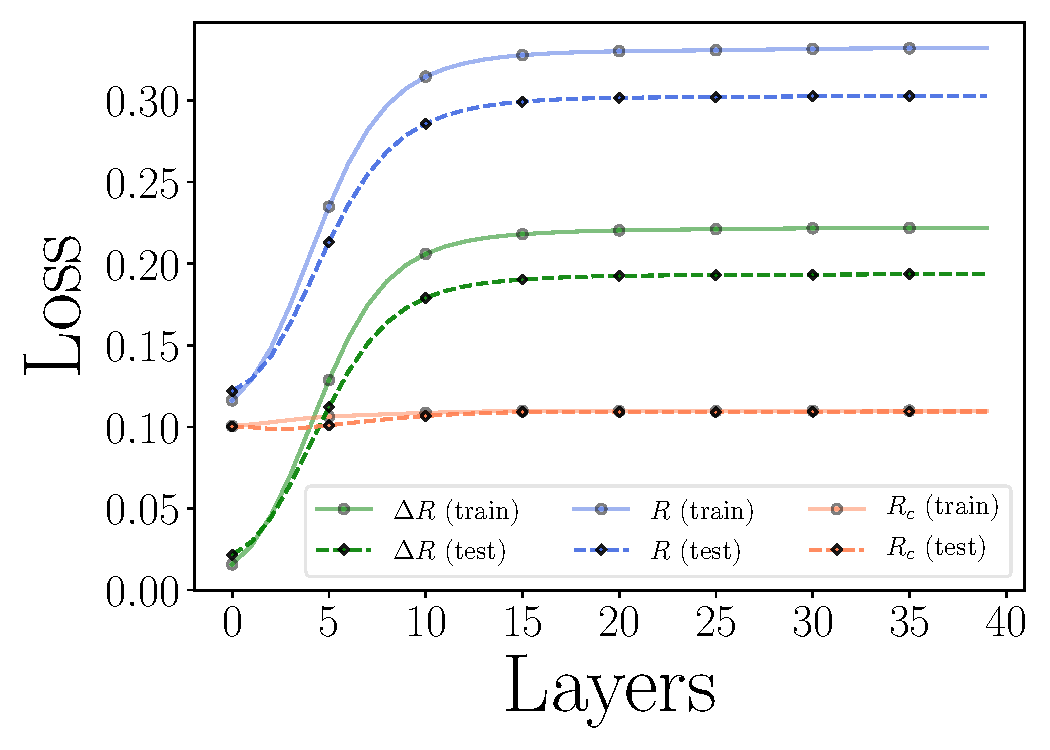
\includegraphics[width=\textwidth]{figs_chap4/mnist1d-loss-traintest.pdf}
        \caption{损失}
    \end{subfigure}
    \caption{\small (a)(b) 是旋转训练数据 $\bm{X}_{\text{rotation}}$ 和学习特征 $\bar{\bm{Z}}_{\text{rotation}}$ 之间余弦相似度的热图,用于旋转不变性。(d) 可视化了训练/验证 MCR$^2$ 损失在各层之间的变化。}
    \label{fig:redu-invariant-1d-mnist-diagram}
\end{figure}

\end{example}






% \begin{figure*}[ht]
%   \begin{center}
%     \subfigure[\label{fig:1d-invariance-plots-a}$\X_{\text{shift}}$ (RI-MNIST)]{
%     \includegraphics[width=0.22\textwidth]{experiments/redunet/mnist1d/class_all/heatmap-X_translate_train_all.pdf}
%     }
%     \subfigure[\label{fig:1d-invariance-plots-b}$\bar{\Z}_{\text{shift}}$ (RI-MNIST)]{
%     \includegraphics[width=0.22\textwidth]{experiments/redunet/mnist1d/class_all/heatmap-Z_translate_train_all.pdf}
%     }
%     \subfigure[\label{fig:1d-invariance-plots-c}相似度 (RI-MNIST)]{
%     \includegraphics[width=0.23\textwidth]{experiments/redunet/mnist1d/class_all/sample_angle_combined-Z-translate_train_all-vs-translate_test_all.pdf}
%     }
%     \subfigure[\label{fig:1d-invariance-plots-d}损失 (RI-MNIST)]{
%     \includegraphics[width=0.23\textwidth]{experiments/redunet/mnist1d/class_all/loss-traintest.pdf}
%     }
%     \vskip -0.1in
%     \subfigure[\label{fig:1d-invariance-plots-e}$\X_{\text{shift}}$ (TI-MNIST)]{
%     \includegraphics[width=0.22\textwidth]{experiments/redunet/mnist2d/class_all/heatmap-X_translate_train_all.pdf}
%     }
%     \subfigure[\label{fig:1d-invariance-plots-f}$\bar{\Z}_{\text{shift}}$ (TI-MNIST)]{
%     \includegraphics[width=0.22\textwidth]{experiments/redunet/mnist2d/class_all/heatmap-Z_translate_train_all.pdf}
%     }
%     \subfigure[\label{fig:1d-invariance-plots-g}相似度 (TI-MNIST)]{
%     \includegraphics[width=0.23\textwidth]{experiments/redunet/mnist2d/class_all/sample_angle_combined-Z-translate_train_all-vs-translate_test_all.pdf}
%     }
%     \subfigure[\label{fig:1d-invariance-plots-h}损失 (TI-MNIST)]{
%     \includegraphics[width=0.23\textwidth]{experiments/redunet/mnist2d/class_all/loss-traintest.pdf}
%     }
%     \vskip -0.1in
%     \caption{\small (a)(b) 和 (e)(f) 分别是平移训练数据 $\X_{\text{shift}}$ 和学习特征 $\bar{\Z}_{\text{shift}}$ 之间余弦相似度的热图,分别用于旋转和平移不变性。
%     (c)(g) 是不同类别之间所有特征对的余弦相似度(绝对值)的直方图:对于每对特征,一个样本来自训练数据集(包括所有平移),另一个样本来自测试数据集中的另一个类别(包括所有可能的平移)。旋转有 $4\times 10^{6}$ 对 (c),平移有 $2.56\times 10^{6}$ 对 (g)。
%     }\label{fig:1d-invariance-plots}
%   \end{center}
%   \vspace{-0.5in}
% \end{figure*}



% \paragraph{频域中的快速计算}
% \yaodong{待办事项:也许删除这部分,只提一下快速计算并引用论文。@Peng Wang。}
% 在 \eqref{eq:def-E-bar} 中计算 $\bar{\bm E}$ 需要对一个大小为 $nC \times nC$ 的矩阵求逆,其复杂度为 $O(n^3C^3)$。
% 通过利用循环矩阵与一维信号的离散傅里叶变换(DFT)之间的关系,可以显著降低这种复杂度。


% 具体来说,令 $\bm F \in \mathbb{C}^{n \times n}$ 为 DFT 矩阵,\footnote{这里我们将矩阵 $\bm F$ 缩放为酉矩阵,因此它与传统的 DFT 矩阵相差一个 $1/\sqrt{n}$ 的因子。} $\mathrm{DFT}(\z) \doteq \bm F \z \in \mathbb{C}^{n \times n}$ 为 $\z \in \Re^n$ 的 DFT,其中 $\mathbb{C}$ 表示复数集。
% 我们知道所有循环矩阵都可以被离散傅里叶变换矩阵 $\bm F$ 同时对角化:
% \begin{equation}
% \label{eq:circ-dft-main}
%     \circm(\z) = \bm F^* \diag(\mathrm{DFT}(\z)) \bm F.
% \end{equation}
% 因此,形式为 \eqref{eqn:W-multichannel} 的协方差矩阵 $\bar{\bm \Sigma}(\bar{\z})$ 可以转换为标准的“对角块”形式:
% \begin{equation}
% \bar{\bm \Sigma}(\bar{\z}) =
% \left[
% \begin{matrix}
% \bm F^* & \bm 0 & \bm 0  \\
% \bm 0 & \footnotesize{\ddots} & \bm 0 \\
% \bm 0 & \bm 0 & \bm F^*
% \end{matrix}
% \right]\left[
% \begin{matrix}
% \bm D_{11}(\bar{\z}) & \cdots & \bm D_{1C}(\bar{\z}) \\
% {\footnotesize \vdots} & {\footnotesize \ddots} & {\footnotesize \vdots} \\
% \bm D_{C1}(\bar{\z}) & \cdots & \bm D_{CC}(\bar{\z})
% \end{matrix}
% \right]\left[
% \begin{matrix}
% \bm F & \bm 0 & \bm 0  \\
% \bm 0 & {\footnotesize \ddots} & \bm 0 \\
% \bm 0 & \bm 0 & \bm F
% \end{matrix}
% \right]\in \Re^{nC \times nC},
% \label{eqn:diagonal-block}
% \end{equation}
% 其中 $\bm D_{cc'}(\bar{\z}) \doteq \diag(\mathrm{DFT}(\z[c])) \cdot \diag(\mathrm{DFT}(\z[c']))^* \in \mathbb{C}^{n \times n}$ 是一个对角矩阵。
% \eqref{eqn:diagonal-block} 右侧的中间部分在行和列置换后是一个块对角矩阵。


% 给定一个多通道特征集合 $\{\bar\z^i \in \Re^{C \times n}\}_{i=1}^m$,我们可以使用 \eqref{eqn:diagonal-block} 中的关系来计算 $\bar{\bm E}$($\bar{\bm C}^j$ 也类似)为
% \begin{equation}
%     \bar{\bm E} =
%     \left[\begin{smallmatrix}
%     \bm F^* & \bm 0 & \bm 0  \\
%     \bm 0 & \footnotesize{\ddots} & \bm 0 \\
%     \bm 0 & \bm 0 & \bm F^*
%     \end{smallmatrix}\right]
%     \cdot \alpha  \left(\I + \alpha \sum_{i=1}^m
%     \left[\begin{smallmatrix}
%     \bm D_{11}(\bar{\z}^i) & \cdots & \bm D_{1C}(\bar{\z}^i) \\
%     {\footnotesize \vdots} & {\footnotesize \ddots} & {\footnotesize \vdots} \\
%     \bm D_{C1}(\bar{\z}^i) & \cdots & \bm D_{CC}(\bar{\z}^i)
%     \end{smallmatrix}\right]
%     \right)^{-1} \cdot
%     \left[\begin{smallmatrix}
%     \bm F & \bm 0 & \bm 0  \\
%     \bm 0 & \footnotesize{\ddots} & \bm 0 \\
%     \bm 0 & \bm 0 & \bm F
%     \end{smallmatrix}\right] \in \Re^{nC \times nC}.
% \end{equation}
% 逆算子中的矩阵在行和列置换后是一个块对角矩阵,有 $n$ 个大小为 $C \times C$ 的块。
% 因此,要计算 $\bar{\bm E}$ 和 $\bar{\C}^j \in \Re^{nC \times nC}$,我们只需要在频域中计算 $n$ 次 $C\times C$ 块的逆,总复杂度为 $O(nC^3)$。\footnote{有强有力的科学证据表明,视觉皮层中的神经元以脉冲发放率编码和传输信息,因此有所谓的脉冲神经元 \cite{spking-neuron-1993,spiking-neuron-book}。大自然可能正在利用频域中的计算效率来实现平移不变性。}

% DFT 计算的优势促使我们在谱域中构建 ReduNet。
% 让我们考虑平移不变特征 $\{\bar\z^i \in \Re^{C \times n}\}_{i=1}^m$ 的\emph{平移不变编码率缩减}目标:
% \begin{multline}
%     \Delta R_\circm(\bar\Z, \bm{\Pi}) \doteq \frac{1}{n}\Delta R(\circm(\bar\Z), \bar{\bm{\Pi}}) = \frac{1}{2n}\log\det \Bigg(\I + \alpha  \circm(\bar\Z)  \circm(\bar\Z)^{*} \Bigg)
%     - \\
%      \sum_{j=1}^{k}\frac{\gamma^{j}}{2n}\log\det\Bigg(\I + \alpha^{j}  \circm(\bar\Z) \bar{\bm{\Pi}}^{j} \circm(\bar\Z)^{*} \Bigg),
% \end{multline}
% 其中 $\alpha = \frac{Cn}{mn\epsilon^{2}} = \frac{C}{m\epsilon^{2}}$,$\alpha^{j} = \frac{Cn}{\textsf{tr}\left(\bm{\Pi}^{j}\right)n\epsilon^{2}} = \frac{C}{\textsf{tr}\left(\bm{\Pi}^{j}\right)\epsilon^{2}}$,$\gamma^{j} = \frac{\textsf{tr}\left(\bm{\Pi}^{j}\right)}{m}$,$\bar{\bm \Pi}^j$ 是以显而易见的方式增强的隶属度矩阵。
% 引入归一化因子 $n$ 是因为循环矩阵 $\circm(\bar\Z)$ 包含每个信号的 $n$ 个(平移)副本。
% 接下来,我们推导用于最大化 $\Delta R_\circm(\bar\Z, \bm{\Pi})$ 的 ReduNet。

% 令 $\mathrm{DFT}(\bar\Z) \in \mathbb{C}^{C \times n \times m}$ 为通过在第二维上进行 DFT 得到的光谱域数据
% %每个信号 $\bar\z^i$ 的每个通道
% 并记 $\mathrm{DFT}(\bar\Z)(p) \in \mathbb{C}^{C \times m}$ 为 $\mathrm{DFT}(\bar\Z)$ 在第二维上的第 $p$ 个切片。
% 那么,$\Delta R_\circm(\bar\Z, \bm{\Pi})$ 关于 $\bar\Z$ 的梯度可以从光谱域中的扩展算子 $\bar\cE \in \mathbb{C}^{C \times C \times n}$ 和压缩算子 $\bar\cC^j \in \mathbb{C}^{C \times C \times n}$ 计算得出,定义为
% \begin{equation}
% \begin{aligned}
%     \bar\cE(p) \doteq&\;  \alpha \cdot \left[\I + \alpha \cdot \mathrm{DFT}(\bar\Z)(p) \cdot \mathrm{DFT}(\bar\Z)(p)^* \right]^{-1} \quad \in \mathbb{C}^{C\times C}, \\
%     \bar\cC^j(p) \doteq& \; \alpha^{j} \cdot\left[\I + \alpha^{j} \cdot \mathrm{DFT}(\bar\Z)(p) \cdot \bm{\Pi}_j \cdot \mathrm{DFT}(\bar\Z)(p)^*\right]^{-1} \quad \in \mathbb{C}^{C\times C}.
% \end{aligned}
% \end{equation}
% 在上式中,$\bar\cE(p)$(相应地,$\bar\cC^j(p)$)是 $\bar\cE$(相应地,$\bar\cC^j$)在最后一个维度上的第 $p$ 个切片。


% \begin{theorem} [计算多通道卷积 $\bar{\bm E}$ 和 $\bar{\bm C}^j$]
% \label{thm:1D-convolution}
% 令 $\bar{\bm U} \in \mathbb{C}^{C \times n \times m}$ 和 $\bar{\bm W}^{j} \in \mathbb{C}^{C \times n \times m}, j=1,\ldots, k$ 由下式给出
% \begin{eqnarray}
%     \bar{\bm U}(p) &\doteq& \bar\cE(p) \cdot \mathrm{DFT}(\bar\Z)(p), \\
%     \bar{\bm W}^{j}(p) &\doteq& \bar\cC^j(p) \cdot \mathrm{DFT}(\bar\Z)(p),
% \end{eqnarray}
% 对于每个 $p \in \{0, \ldots, n-1\}$。那么,我们有
% \begin{eqnarray}
%     \frac{1}{2n}\frac{\partial \log \det (\I + \alpha \cdot \circm(\bar\Z) \circm(\bar\Z)^{*} )}{\partial \bar\Z} &=& \mathrm{IDFT}(\bar{\bm U}),
%     \\
%     \frac{\gamma^{j}}{2n}\frac{\partial  \log\det (\I + \alpha^{j} \cdot \circm(\bar\Z) \bm \bar{\bm \Pi}^j \circm(\bar\Z)^{*})}{\partial \bar\Z}&=&
%     \gamma^{j} \cdot \mathrm{IDFT}(\bar{\bm W}^{j} \bm \Pi^j).
% \end{eqnarray}
% 在上式中,$ \mathrm{IDFT}(\bar{\bm U})$ 是通过对 $\bar{\bm U}$ 中每个信号的每个通道进行逆 DFT 得到的时域信号。
% \end{theorem}
% 根据这个结果,\eqref{eqn:gradient-descent} 中的梯度上升更新(当应用于目标 $\Delta R_\circm(\bar\Z, \bm{\Pi})$ 时)可以等价地表示为在谱域上对 $\bar{\bm V}_\ell \doteq \mathrm{DFT}(\bar\Z_\ell)$ 的更新
% \begin{equation}
%     \bar{\bm V}_{\ell+1}(p) \; \propto \; \bar{\bm V}_{\ell}(p) + \eta \; \Big(\bar\cE_\ell(p) \cdot \bar{\bm V}_\ell(p) - \sum_{j=1}^k \gamma^{j} \bar\cC_\ell^j(p) \cdot \bar{\bm V}_\ell(p) \bm \Pi^j \Big), \quad p = 0, \ldots, n-1,
% \end{equation}
% 并且可以像之前一样构建一个 ReduNet。




\section{通过展开优化构建白盒 Transformer}\label{sec:chap4-white-box-transformer}
正如我们在上一节所见,我们使用分类问题为 ResNet 和 CNN 等流行深度网络的主要架构特性提供了严格的解释:这类网络的每一层都可以被看作是模仿一个增加率缩减(或信息增益)目标的梯度步骤。这一视角也引出了一个有些令人惊讶的事实:这样一个深度网络(ReduNet)的层参数和算子可以以纯粹的前向方式计算。

尽管 ReduNet 在理论和概念上具有重要意义,但有几个因素限制了它的实际应用。首先,正如我们上面讨论的,以纯前向方式计算每一层中的矩阵算子的计算成本可能非常高。其次,如此计算出的算子在优化目标方面可能不那么有效,可能需要数千次迭代(即层数)。正如我们在第 \ref{ch:classic} 章的 \ref{sec:LISTA} 节中对 LISTA 所见,这两个问题可以通过允许优化这些算子并通过反向传播等方式使其可学习来解决。\footnote{或者可能通过前向和后向优化的混合方式。}

ReduNet 所推导出的监督分类设置也有些局限性。在实践中,一张图像可能不只属于一个类别,因为它可能包含多个物体。因此,假设图像的不同区域属于不同的低维模型(例如高斯模型或子空间)会更具一般性。正如我们将看到的,这种泛化将导出一个既简单又通用的架构,它统一了我们在前一章中看到的率缩减和去噪操作。此外,如此获得的架构与流行的 Transformer 架构相似。

% \pw{待办事项:从 ReduNet(理想情况)到一般情况(不是每个样本都有唯一标签)的过渡。从监督学习到无监督学习}
% \yaodong{写一段话,激励更高效的白盒模型设计(在 ReduNet 中我们需要计算矩阵的逆,扩展性不强);同时激励无监督情况,不是对每个样本建模,而是可以对(一个样本中的)每个补丁建模,认为其来自高斯混合模型。}

% \subsection{CRATE}

\subsection{稀疏率缩减的展开优化}

% 简要回顾第 \ref{ch:linear-independent} 章中的稀疏字典学习问题,对其展开优化进行微调可以得到学习型 ISTA (LISTA) 架构。来自展开卷积稀疏恢复的 sparseLand 型网络...

% \pw{待办事项:通过统一率缩减、去噪和扩散以及 Transformer,我们推导出了\href{https://arxiv.org/abs/2306.01129}{白盒 Transformer CRATE}。}

我们考虑一个与现实世界信号相关的一般学习设置。令 \(\X = \mat{\x_{1}, \dots, \x_{N}} \in \bR^{D \times N}\) 表示代表我们数据源的随机变量。在视觉任务中,每个 \(\x_{i} \in \bR^{D}\) 被解释为一个\textit{令牌},通常对应一个图像块。在语言任务中,每个 \(\x_{i} \in \bR^{D}\) 被解释为一个\textit{令牌嵌入},即一个离散令牌(如单词或子词)的连续向量表示。\footnote{为方便起见,本章中我们不严格区分,将离散令牌及其相关嵌入统称为令牌。} % \footnote{对于语言 Transformer,令牌大致对应于单词~\cite{vaswani2017attention},而对于视觉 Transformer,令牌对应于图像块~\cite{dosovitskiy2020image}。}
\(\x_{i}\) 之间可以有任意的相关结构。我们用 \(\Z = \mat{\z_{1}, \dots, \z_{N}} \in \bR^{d \times N}\) 来表示定义我们表示的随机变量,其中 \(\z_{i} \in \bR^{d}\) 是相应令牌 \(\x_i \in \bR^{D}\) 的表示。% 我们给定 \(B \geq 1\) 个独立同分布的样本 \(\X_{1}, \dots, \X_{B} \sim \X\),其令牌为 \(\x_{i, b}\)。我们样本的表示记为 \(\Z_{1}, \dots, \Z_{B} \sim \Z\),令牌的表示为 \(\z_{i, b}\)。最后,对于一个给定的网络,我们用 \(\Z^{\ell}\) 表示当输入为 \(\X\) 时前 \(\ell\) 层的输出。相应地,样本输出为 \(\Z_{i}^{\ell}\),令牌输出为 \(\z_{i, b}^{\ell}\)。

\begin{remark}
    在 Transformer 中,每个输入样本通常被转换成一个{\em 令牌}序列。令牌是从原始输入中导出的基本信息单元:在自然语言处理中,令牌通常是单词或子词;在计算机视觉中,它们对应于图像块;在其他模态中,它们可能代表时间步、空间位置或其他领域特定的单元。{\em 令牌嵌入}是令牌的连续向量表示,作为 Transformer 的输入。它将每个令牌映射到高维空间中的一个点,使模型能够使用数值计算来处理符号输入。
    {\em 令牌表示}是一个编码令牌语义或结构信息的向量,通常由 Transformer 的中间层或最终层产生。这些表示旨在捕获对下游任务(如分类、生成或回归)有用的输入特征。有关这些概念在实现中的更多细节,请参阅 \Cref{sec:contrastive_learning}。
\end{remark}


% \paragraph{通过简约与一致性原则进行表示学习。} 遵循 \Cref{sec:chap4-white-box-model-via-unrolling} 中的率缩减框架,我们主张表示学习的目标是找到一个特征映射 \(f \colon \vX \in \bR^{D \times N} \to \vZ\in \bR^{d \times N}\),它将具有潜在非线性和多模态分布的输入数据 \(\vX \in \bR^{D \times N}\) 转换为一个结构化和紧凑的特征表示 \(\vZ \in \bR^{d \times N}\) \citep{ma2022principles}。

\paragraph{学习结构化和紧凑表示的目标。}
遵循 \Cref{sec:chap4-white-box-model-via-unrolling} 中的率缩减框架,我们主张表示学习的目标是找到一个特征映射 \(f \colon \X \in \bR^{D \times N} \to \Z\in \bR^{d \times N}\),它将具有潜在非线性和多模态分布的输入令牌 \(\{\bm x_i\}_{i=1}^N \subset \R^D\) 转换为一个(分段)\textit{线性化和紧凑}的令牌表示 \(\{\bm z_i\}_{i=1}^N \subset \bR^{d}\)。虽然令牌表示 \(\{\z_{i}\}_{i = 1}^{N}\) 的联合分布可能很复杂(且与任务相关),但我们进一步主张,要求单个令牌表示的目标边际分布是高度压缩和结构化的,适合紧凑编码,是合理且实用的。特别地,我们要求该分布是\textit{低维(比如 \(K\) 个)高斯分布的混合},使得第 \(k\) 个高斯分布的均值为 \(\Zero \in \bR^{d}\),协方差为 \(\vSigma_{k} \succeq \Zero \in \bR^{d \times d}\),其支撑集由正交基 \(\vU_{k} \in \bR^{d \times p}\) 张成。
我们用 $\vU_{[K]} = \{\vU_k\}_{k=1}^K$ 表示所有高斯分布的基集合。因此,为了最大化最终令牌表示的\textit{信息增益} \cite{ma2022principles},我们希望最大化它们的率缩减(见 \Cref{subsec:MCR2}),即
\begin{align}\label{eq:rate reduction}
    \mathrm{max}_{\bm Z \in \R^{d\times N}}\ \Delta R_{\epsilon}(\Z \mid \vU_{[K]}) \doteq R_{\epsilon}(\Z) - R^c_{\epsilon}(\Z \mid \vU_{[K]}).
\end{align}
%即 $\max_{\Z} \Delta R(\Z; \vU_{[K]}) = R(\Z) - R^c(\Z; \vU_{[K]})$,
% 其中 \(R\) 和 \(R^{c}\) 是有损编码率的估计,将在公式 \eqref{eq:coding_rate} 和 \eqref{eq:def-mcr-Rc} 中正式定义。这也促进了来自不同高斯分布的令牌表示 \(\z_{i}\) 变得\textit{不相干} \cite{yu2020learning}。
这里,第一项 $R_{\epsilon}$ 是整个令牌表示集合的有损编码率的估计。更具体地说,如果我们将令牌表示 $\{\bm z_i\}_{i=1}^N$ 视为从一个零均值高斯分布中抽取的独立同分布样本,那么在量化精度 $\epsilon > 0$ 的条件下,它们的有损编码率为
\begin{equation}\label{eq:coding_rate}
    R_{\epsilon}(\Z) \doteq \frac{1}{2}\textrm{logdet}\left(\I + \frac{d}{N\epsilon^{2}}\Z^{\top}\Z\right) = \frac{1}{2}\textrm{logdet}\left(\I + \frac{d}{N\epsilon^{2}}\Z\Z^{\top}\right).
\end{equation}
第二项 $R_{\epsilon}^c$ 是在码本 $\bm U_{[K]}$ 下的有损编码率的估计,由下式给出
\begin{equation}
\begin{aligned}
    R_{\epsilon}^c(\Z \mid \vU_{[K]}) &\doteq \sum_{k=1}^{K}R_{\epsilon}(\vU_k^{\top} \Z) = \frac{1}{2}\sum_{k=1}^{K}\log\det\left(\I +
    \frac{p}{N\epsilon^{2}}(\vU_k^{\top}\Z)^{\top}(\vU_k^{\top}\Z)\right).
\end{aligned}
\label{eq:def-mcr-Rc}
\end{equation}

\begin{remark}
    编码率的表达式 \eqref{eq:def-mcr-Rc} 可以看作是原始率缩减目标 \eqref{eq:MCRc} 中使用的编码率 \(R_\epsilon^{c}\) 的推广。特别是,原始目标是针对特定数据实现 \(\vX\) 的一组已知隶属度标签 \(\{\vPi_{k}\}\) 定义的。相比之下,当前目标是针对子空间 \(\vU_{[K]}\) 定义的,这些子空间独立于任何特定的实现,但被假定为支持令牌表示的分布。假设一个令牌表示 $\bm z_i$ 属于一个子空间 $\bm U_k$,并且这些子空间彼此近似正交,即对于所有 $k \neq l$,$\bm U_k^\top \bm U_l \approx \bm 0$。那么,可以验证投影 $\bm U_k\bm U_k^\top \bm z_i  = \bm z_i$ 和对于所有 $l \neq k$,$\bm U_l\bm U_l^\top \bm z_i \approx \bm 0$。这些正交投影有效地充当了隐式的隶属度标签,识别出每个令牌表示所属的子空间。
\end{remark}

% \begin{figure}
%     \centering
%     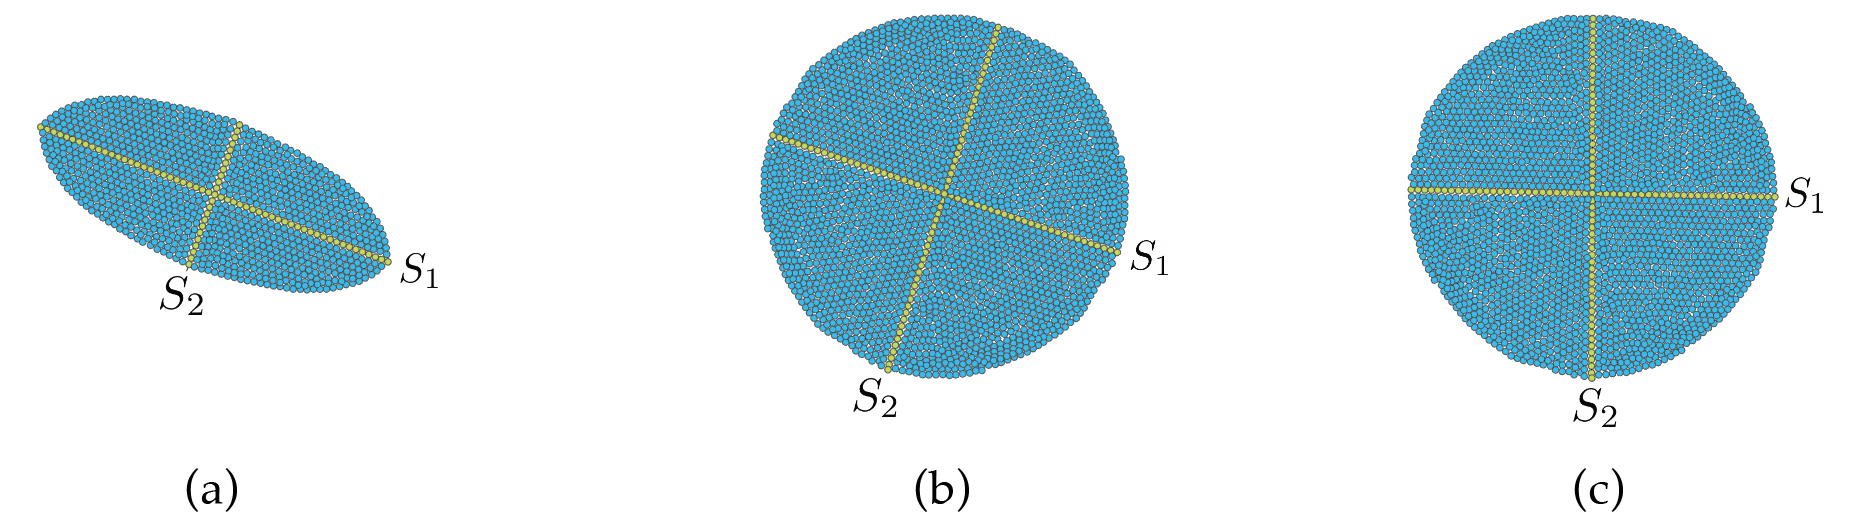
\includegraphics[width=0.95\textwidth]{figs_chap4/image_eps_ball.png}
%     \vspace{-0.1in}\caption{\small\textbf{通过率缩减和稀疏性比较三组表示。} 每个 $S_i$ 代表一个线性子空间,蓝色球的数量代表编码率之间的差异 $\Delta R_{\epsilon}(\vZ \mid \vU_{[K]})$。}
%     \label{fig:diagram_compare_compression_sparsification}
% \end{figure}


\begin{figure}[t!]
     \centering
         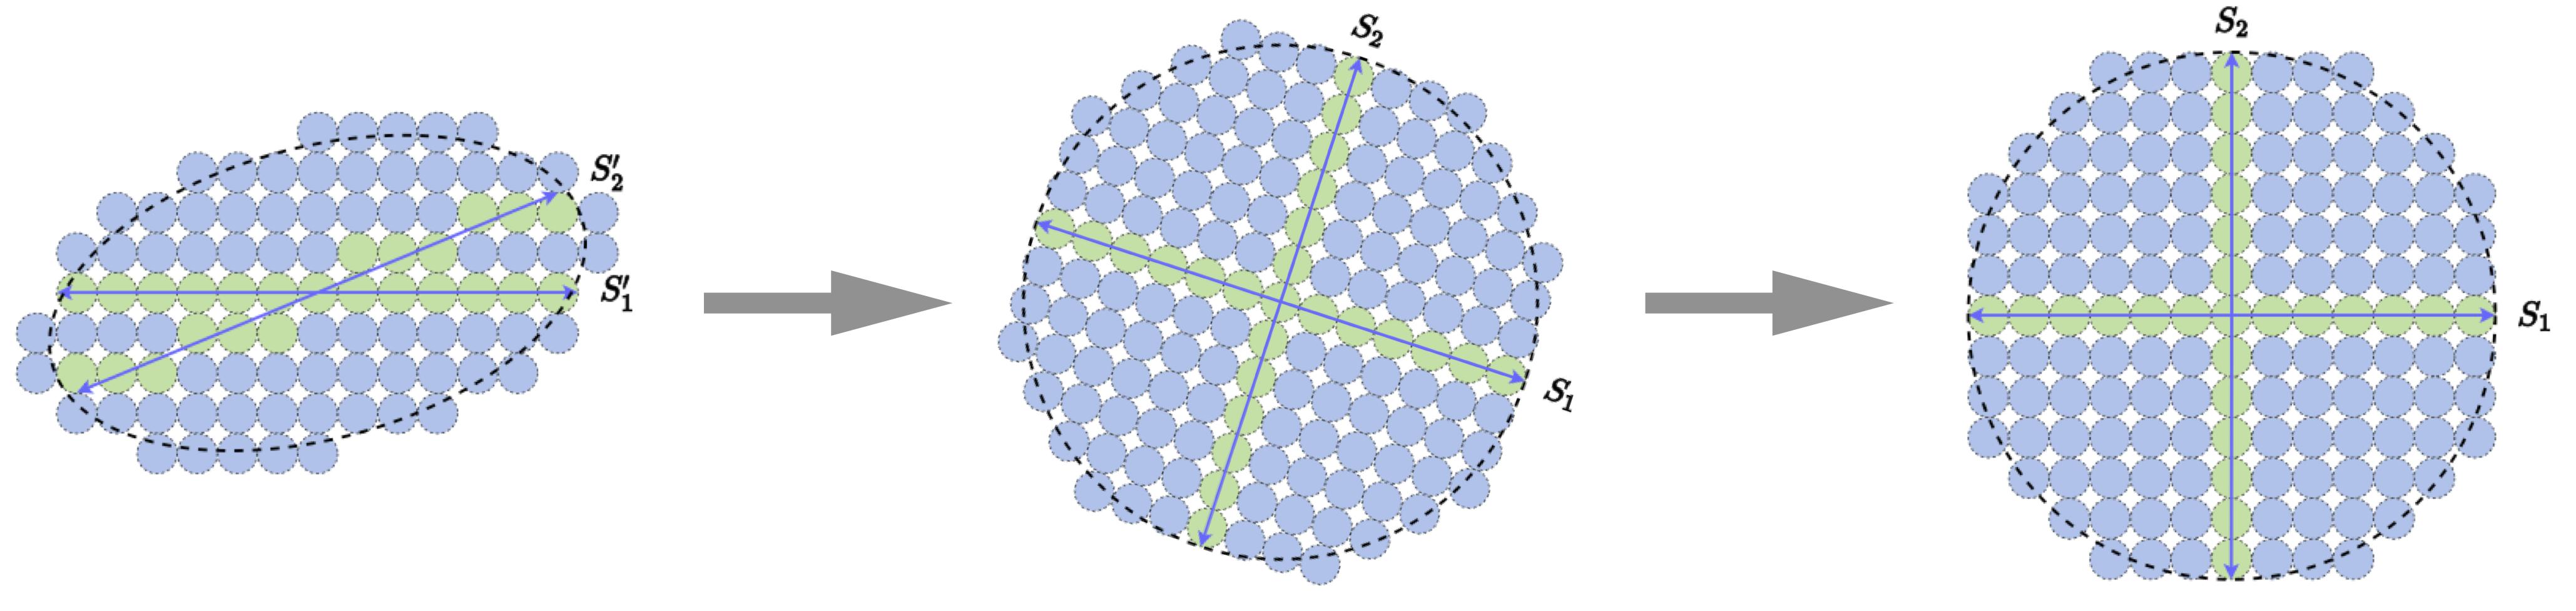
\includegraphics[width=0.95\textwidth]{figs_chap4/coding-transform.png}
     \caption{ \small\textbf{通过率缩减和稀疏性比较三组表示。} 每个 $S_i$ 代表一个线性子空间,蓝色球的数量代表编码率之间的差异 $\Delta R_{\epsilon}(\vZ \mid \vU_{[K]}) = R_\epsilon(\vZ) - R^c_\epsilon(\vZ \mid \vU_{[K]})$。
     }
        \label{fig:sparse-rate-reduction-diagram}
\end{figure}


\paragraph{稀疏率缩减。} 请注意,率缩减目标 \eqref{eq:rate reduction} 对表示和子空间的任意联合旋转是不变的。特别是,优化率缩减目标可能不会自然地导致轴对齐(即\textit{稀疏})的表示。{例如,考虑 \Cref{fig:sparse-rate-reduction-diagram} 中的三组学习表示。编码率缩减从 (a) 到 (b) 增加,但由于它在旋转下是不变的,所以从 (b) 到 (c) 保持不变。} 因此,我们希望变换表示(及其支撑子空间),使得表示 $\vZ$ 最终相对于所得表示空间的标准坐标系变得稀疏\footnote{具体来说,就是具有很少的非零项。}{如 \Cref{fig:sparse-rate-reduction-diagram}(c) 所示}。因此,为了确保最终的表示适合更紧凑的编码,我们希望变换表示(及其支撑子空间),使它们相对于所得表示空间的标准坐标系变得\textit{稀疏}。\footnote{也就是说,具有最少的非零项。} 在计算上,我们可以将上述两个目标合并为一个统一的优化目标:
\begin{equation}
   \max_{f \in \mathcal{F}}\ \Delta R_{\epsilon}(\Z \mid \vU_{[K]}) - \lambda \|\bm{Z}\|_0 \qquad \text{s.t.}\ \Z = f(\X),
   \label{eq:sparse-rr}
\end{equation}
其中 $\mathcal{F}$ 表示一个通用的函数类,$\ell_0$-范数 $\|\Z\|_0$ 促进最终令牌表示 \(\Z = f(\X)\) 的稀疏性。% \footnote{为了简化符号,我们将一次讨论一个样本 $\X$ 的目标,并理解我们总是意味着优化期望。} 我们称这个目标为\textit{稀疏率缩减}。
% \yima{一个图来说明稀疏率缩减目标...}
% \yaodong{添加了下面的图以及与 MCR$^2$ 的比较。}

% 我们提供了一个稀疏率缩减目标的示意图(图 \ref{fig:sparse-rate-reduction-diagram}),并将其与前面介绍的 MCR$^2$ 目标进行了比较。
% 很容易看出,率缩减目标,即在公式 \ref{eqn:maximal-rate-reduction} 中定义的 MCR$^2$,对表示和子空间的任意联合旋转是不变的。
% 特别是,优化率缩减可能不会自然地导致轴对齐(即\textit{稀疏})的表示。{例如,考虑图 \ref{fig:sparse-rate-reduction-diagram} 中的三组学习表示。编码率缩减从 (a) 到 (b) 增加,但由于它在旋转下是不变的,所以从 (b) 到 (c) 保持不变。} 因此,我们希望变换表示(及其支撑子空间),使得特征 $\vZ$ 最终变得稀疏——即相对于所得表示空间的标准坐标系具有很少的非零项{如图 \ref{fig:sparse-rate-reduction-diagram}(c) 所示}。

在实践中,$\ell_0$-范数通常被松弛为 $\ell_1$-范数,以提高计算的可追踪性并启用凸优化技术 \cite{Wright-Ma-2022}。受此启发,我们相应地松弛问题 \eqref{eq:sparse-rr},得到一个既忠实于原始稀疏性目标又更适合高效算法的公式如下:
\begin{equation}
\begin{aligned}
   \max_{f \in \mathcal{F}}\    \Delta R_{\epsilon}(\Z \mid \vU_{[K]}) - \lambda \|\bm{Z}\|_1  \qquad \text{s.t.}\ \Z = f(\X),
   \label{eq:sparse-rr-1}
\end{aligned}
\end{equation}
为方便起见,我们通常也将这个目标函数称为\textit{稀疏率缩减}。

\paragraph{通过展开优化的白盒网络架构。}

% 为了优化学习目标并学习紧凑和结构化的表示,一种方法是展开优化~\cite{gregor2010learning,tolooshams2021stable}:深度网络的每一层实现一个优化学习目标的迭代算法。
% 例如,可以设计层 $f^{\ell}$,使得前向传播等价于优化学习目标 $L(\vZ)$ 的一个近端梯度下降步骤,即 $\vZ^{\ell+1} = f^{\ell}(\vZ^{\ell}) = \texttt{Prox}[\vZ^{\ell} - \eta\cdot\nabla_{\vZ} L(\vZ^{\ell})]$。这里我们用 $\eta$ 表示步长,用 $\texttt{Prox}[\cdot]$ 表示近端算子~\cite{parikh2014proximal}。

尽管表述简单,但上述目标中的每一项在计算上都具有挑战性 \cite{Wright-Ma-2022}。因此,采用一种近似方法,通过连接多个(比如 $L$ 个)简单的\textit{增量和局部}操作 $f^\ell$ 来实现全局变换 $f$ 以优化 \eqref{eq:sparse-rr} 是很自然的,这些操作将表示分布推向期望的简约模型分布:
\begin{equation}
f\colon \X = \bm Z^0 \xrightarrow{\hspace{1mm} f^0 \hspace{1mm}} \Z^1 \rightarrow \cdots \rightarrow \Z^\ell \xrightarrow{\hspace{1mm} f^{\ell} \hspace{1mm}} \Z^{\ell+1} \rightarrow  \cdots \xrightarrow{\hspace{1mm} f^{L-1}} \Z^L = \Z,
\label{eq:incremental}
\end{equation}
其中 $f^0: \bR^{D} \rightarrow \bR^{d}$ 是预处理映射,它将每个输入令牌 $\x_{i} \in \bR^{D}$ 转换为初始令牌表示 $\z_{i}^{1} \in \bR^{d}$。
每个增量\textit{前向映射} $\Z^{\ell + 1} = f^\ell(\Z^\ell)$,或称为一个“层”,都会变换令牌分布以\textit{优化}上述稀疏率缩减目标 \eqref{eq:sparse-rr},这取决于其输入 $\Z^\ell$ 的分布。

\begin{remark}
    与其他展开优化方法(如 ReduNet,见 \Cref{sec:chap4-white-box-model-via-unrolling})相比,我们\textit{显式地建模}每一层 $\Z^\ell$ 的分布,例如,作为一个线性子空间混合或从一个字典中稀疏生成。模型参数是从数据中学习的(例如,通过端到端训练的\textit{反向传播})。这种前向“优化”和后向“学习”之间的分离,阐明了每一层作为一个算子的数学作用,该算子变换其输入的分布,而输入分布又由该层的参数建模(并随后学习)。
\end{remark}

现在,我们展示如何通过展开优化的视角来推导这些增量和局部操作,以解决问题 \eqref{eq:sparse-rr-1}。一旦我们决定使用增量方法来优化问题 \eqref{eq:sparse-rr-1},就有多种可能的选择来实现优化。给定一个 $\Z^\ell$ 的模型,比如子空间混合 $\vU_{[K]}$,我们选择一个具有强大概念基础的两步\textit{交替最小化}方法。首先,我们通过梯度下降来\textit{压缩}令牌 $\vZ^{\ell}$,以最小化编码率项 $R^c_\epsilon (\vZ \mid \vU_{[K]}^\ell)$。具体来说,我们对 $R^c_\epsilon$ 进行一个学习率为 $\kappa$ 的梯度步骤,如下所示:
\begin{align}\label{eq:Z l+1/2}
    \bm Z^{\ell+1/2} = \bm Z^\ell - \kappa \nabla_{\bm Z} R^c_\epsilon (\vZ \mid \vU_{[K]}^\ell).
\end{align}
接下来,我们\textit{稀疏化}压缩后的令牌,通过一个适当松弛的近端梯度步骤来生成 \(\vZ^{\ell + 1}\),以最小化剩余项 $\lambda \norm{\vZ}_{1} - R_{\epsilon}(\vZ)$。正如我们稍后将详细论证的,我们可以通过解决一个关于字典 $\bm D^\ell$ 的稀疏表示问题来找到这样的 $\bm Z^{\ell+1}$:
\begin{equation}\label{eq:Z l+1}
  \vZ^{\ell+1} = \argmin_{{\vZ}}  \lambda \norm{\vZ}_1 + \frac{1}{2}\norm{\vZ^{\ell + 1/2} - \vD^{\ell} {\vZ}}_F^2.
\end{equation}
在下文中,我们为上述两个步骤中的每一步提供技术细节,并推导出它们实现的高效更新。




\paragraph{自注意力作为令牌表示编码率的梯度下降。} 对于第一步 \eqref{eq:Z l+1/2},编码率的梯度 \(\nabla_{\bm Z} R^c_\epsilon\) 计算成本很高,因为它涉及 \(K\) 个独立的矩阵求逆,每个求逆对应 \(K\) 个子空间中的一个,其基为 \(\vU_{k}^{\ell}\):
\begin{equation}
    \nabla_{\bm Z} R_{\epsilon}^c(\vZ \mid \vU_{[K]})
    = \frac{p}{N\epsilon^2}\sum_{k=1}^K \vU_k\vU_k^\top\vZ\Big(\I +
    \frac{p}{N\epsilon^2}(\vU_k^\top\vZ)^\top(\vU_k^\top\vZ)\Big)^{-1}.
    \label{eq:rate-gradient}
\end{equation}
现在,我们证明这个梯度可以自然地用一个所谓的“多头子空间自注意力”(MSSA)算子来近似,该算子与多头自注意力算子 \citep{vaswani2017attention} 具有相似的函数形式,其中有 \(K\) 个头(即每个子空间一个,来自每个矩阵求逆)。这里,我们使用一阶诺伊曼级数(见 \Cref{ex:neumannn})来近似梯度 \eqref{eq:rate-gradient}:
\begin{align}\label{eq:gd_rc_neumann}
    \nabla_{\bm Z} R_{\epsilon}^{c}(\vZ \mid \vU_{[K]})
    &\approx \frac{p}{N\epsilon^2} \sum_{k = 1}^{K}\vU_{k}\vU_{k}^\top\vZ\left(\vI - \frac{p}{N\epsilon^2} (\vU_{k}^\top\vZ)^\top(\vU_{k}^\top\vZ)\right) \notag \\
    &{= \frac{p}{N\epsilon^2} \left(\sum_{k = 1}^{K} \vU_{k}\vU_{k}^\top\right)\vZ -  \left( \frac{p}{N\epsilon^2}\right)^2\sum_{k = 1}^{K} \vU_{k}(\vU_{k}^\top\vZ)(\vU_{k}^\top\vZ)^\top(\vU_{k}^\top\vZ)}.
\end{align}
在这个近似中,我们通过投影特征之间的自相关 $(\vU_{k}^\top\vZ)^\top(\vU_{k}^\top\vZ)$ 来计算投影令牌表示 $\{\bm U_k^\top\bm z_i\}$ 之间的相似度,并用 softmax 将其转换为隶属度分布,即 $\softmax{(\vU_{k}^\top\vZ)^\top(\vU_{k}^\top\vZ)}$。
假设子空间的并集 $\bm U_{[K]}$ 张成整个空间。那么,我们有 $\sum_{k = 1}^{K} \vU_{k}\vU_{k}^\top = \bm I$。因此,\eqref{eq:gd_rc_neumann} 变为
\begin{align}\label{eq:grad Rc}
    \nabla_{\bm Z} R_{\epsilon}^{c}(\vZ \mid \vU_{[K]})
     \approx  \frac{p}{N\epsilon^2} \vZ -  \left( \frac{p}{N\epsilon^2}\right)^2 \MSSA\left(\vZ^{\ell} \mid \vU_{[K]}^{\ell}\right),
\end{align}
其中 MSSA 通过一个 SSA 算子定义如下:
\begin{align}
% \vspace{-0.15in}
    & \mathrm{SSA}\left(\vZ \mid \vU_{k}\right)
    \doteq (\vU_{k}^\top \vZ)\mathrm{softmax}\left((\vU_{k}^\top\vZ)^\top(\vU_{k}^\top\vZ)\right), \ \forall k \in [K], \label{eq:SSA} \\
    & \mathrm{MSSA}\left(\vZ \mid \vU_{[K]}\right)
    \doteq \frac{p}{N\epsilon^2} \mat{\vU_{1}, \dots, \vU_{K}}\mat{\mathrm{SSA}({\vZ \mid \vU_{1}}) \\ \vdots \\ \mathrm{SSA}({\vZ \mid \vU_{K}})}.\label{eq:Multi-Head-SSA}
\end{align}
将 \eqref{eq:grad Rc} 代入 \eqref{eq:Z l+1/2} 得到,它可以自然地被近似为
\begin{equation}
    \vZ^{\ell + 1/2} = \left(1 - \frac{\kappa p}{N\epsilon^2}\right) \vZ^{\ell} + \frac{\kappa p}{N\epsilon^2} \mathrm{MSSA}\left({\vZ^{\ell} \mid \vU_{[K]}^{\ell}}\right).  \label{eq:gd-mcr-parts}
\end{equation}
% 接下来,我们\textit{稀疏化}压缩后的令牌,通过一个适当松弛的近端梯度步骤,对稀疏性惩罚项和扩展项的差值进行操作,以最小化剩余项 $\lambda \norm{\vZ}_{1} - R_\epsilon(\vZ)$。
% \begin{align}
%     \bm Z^{l+1} = \mathrm{argmin}\ \frac{1}{2} \left\| \bm Z^{\ell+1/2} - \bm D^\ell\bm Z \right\|_F^2 + \lambda \|\bm Z_1\|.
% \end{align}
% 这两个算子被增量地、重复地应用,因为 \eqref{eq:incremental} 中的每个 $f^\ell$ 都是通过这两个步骤实例化的。



\begin{remark}
    \eqref{eq:SSA} 中的 SSA 算子类似于典型 Transformer \citep{vaswani2017attention} 中的\textit{注意力算子},不同之处在于这里的值、键和查询的线性算子都\textit{与}子空间基\textit{相同},即 $\vV_{k} = \vK_{k} = \bm{Q}_{k} = \vU_k^*$。因此,我们将 $\mathrm{SSA}({\spcdot\mid\vU_k}): \bR^{d\times n} \rightarrow \bR^{p\times n}$ 命名为\textbf{子空间自注意力}(\textbf{S}ubspace \textbf{S}elf-\textbf{A}ttention, SSA)算子。然后,\eqref{eq:Multi-Head-SSA} 中的整个 MSSA 算子,正式定义为 \(\mathrm{MSSA}({\spcdot \mid \vU_{[K]}}) \colon \bR^{d \times n} \to \bR^{d \times n}\) 并称为\textbf{多头子空间自注意力}(\textbf{M}ulti-Head \textbf{S}ubspace \textbf{S}elf-\textbf{A}ttention, MSSA)算子,它通过使用依赖于模型的权重来聚合注意力头的输出,这在概念上类似于现有 Transformer 网络中流行的多头自注意力算子。整个梯度步骤 \eqref{eq:gd-mcr-parts} 类似于 Transformer 中通过跳跃连接实现的多头自注意力。
\end{remark}




\paragraph{MLP 作为令牌表示稀疏编码的近端梯度下降。} 对于交替最小化的第二步,我们需要最小化 $\lambda \norm{\vZ}_{1} - R_{\epsilon}(\vZ)$。注意,梯度 \(\nabla R_{\epsilon}(\vZ)\) 涉及矩阵求逆,因此使用朴素的近端梯度(见 \Cref{subsec:pgd})来优化这个问题在大规模问题上变得难以处理。% 然而,这个问题是高度非光滑和非凸的,难以优化。
因此,我们采取一种不同的、简化的方法来权衡表示多样性和稀疏化:我们假设一个(完备的)不相干或正交字典 $\vD^{\ell} \in \bR^{d \times d}$,并要求对中间迭代 $\vZ^{\ell + 1/2}$ 进行稀疏化,使其相对于 \(\vD^{\ell}\) 稀疏。也就是说,$\vZ^{\ell + 1/2} \approx \vD^{\ell} \vZ^{\ell + 1}$,其中 $\vZ^{\ell + 1}$ 更稀疏;也就是说,它是 \(\vZ^{\ell + 1/2}\) 的一个\textit{稀疏编码}。字典 \(\vD^{\ell}\) 用于同时稀疏化所有令牌。
根据不相干性假设,我们有 $(\vD^{\ell})^\top(\vD^{\ell}) \approx \vI$。因此从 \eqref{eq:coding_rate} 我们有
\begin{equation}
    R_{\epsilon}(\vZ^{\ell + 1/2}) \approx R_{\epsilon}(\vD^{\ell}\vZ^{\ell + 1}) \approx R_{\epsilon}(\vZ^{\ell + 1}).
\end{equation}
为了解决 $\lambda \norm{\vZ}_{1} - R_{\epsilon}(\vZ)$,我们优化以下问题
\begin{align*}
       \vZ^{\ell + 1} \approx \argmin_{\vZ}  \norm{\vZ}_1 \quad \mbox{subject to} \quad \vZ^{\ell + 1/2} = \vD^{\ell}\vZ.
\end{align*}
{上述稀疏表示程序通常通过将其松弛为一个无约束的凸规划来解决,这被称为 LASSO \citep{Wright-Ma-2022}:}
\begin{equation}
    \vZ^{\ell + 1} \approx \argmin_{\vZ} \left[\lambda \norm{\vZ}_1 + \frac{1}{2}\norm{\vZ^{\ell + 1/2} - \vD^{\ell} \vZ}_F^2 \right].
\end{equation}
在我们的实现中,我们还对 $\vZ^{\ell + 1}$ 添加了一个非负约束,并解决相应的非负 LASSO 问题:
\begin{equation}
    \vZ^{\ell + 1} \approx \argmin_{\vZ \geq \bm 0} \left[\lambda\norm{\vZ}_1 + \frac{1}{2}\norm{\vZ^{\ell + 1/2} - \vD^{\ell} \vZ}_{F}^{2}\right].
    \label{eq:sparse-nonnegative}
\end{equation}
然后,我们通过执行一个展开的{\em 近端梯度下降}步骤,即一个 ISTA 步骤 \citep{beck2009fast},来增量地优化 \Cref{eq:sparse-nonnegative},得到更新:
\begin{align}\label{eq:ista-block}
    \vZ^{\ell + 1}
    &= \mathrm{ISTA}({\vZ^{\ell + 1/2} \mid \vD^{\ell}}), \\
    \text{其中} \quad \mathrm{ISTA}({\vZ \mid \vD})
    &\doteq \operatorname{ReLU}(\vZ - \eta \vD^\top(\vD\vZ - \vZ) - \eta \lambda \bm{1}).
\end{align}

% \paragraph{\textsc{CRATE} 模型的一层} 我们现在设计一个白盒 Transformer 架构,命名为编码率 Transformer (\textsc{crate}),通过对稀疏率缩减目标 \eqref{eq:sparse-rr} 进行展开优化。 \textsc{crate} 的每一层包含两个块:压缩块和稀疏化块,它们对应于优化稀疏率缩减目标 \eqref{eq:sparse-rr} 的一个两步交替优化过程。


% 具体来说,\textsc{crate} 的第 $\ell$ 层定义为
% \begin{equation}
%     \vZ^{\ell+1} = f^{\ell}(\vZ^{\ell}) = {\texttt{ISTA}(\vZ^{\ell+1/2}\,|\,\vD^{\ell})},\, \mathrm{其中}\ \vZ^{\ell + 1/2}
%     = \vZ^{\ell} + \MSSA(\vZ^{\ell}).
% \end{equation}

% \textbf{{压缩块 MSSA。}}
% \textsc{crate} 中的压缩块,称为\textbf{多}头\textbf{子空间}\textbf{自注意力}块(\(\MSSA\)),是通过优化压缩项 $R_\epsilon^c$(在 \eqref{eq:def-mcr-Rc} 中定义)来压缩令牌集 $\vZ=[\vz_1, \dots, \vz_{N}]$ 而推导出来的,即
% \begin{align}\label{eq:grad_rc_mssa}
%     \vZ^{\ell + 1/2}
%     &= \vZ^{\ell} + \MSSA(\vZ^{\ell} \mid \vU_{[K]}^{\ell}) \approx \vZ^{\ell} - \kappa \nabla_{\vZ}R^{c}(\vZ^{\ell}\,|\,\vU_{[K]}^{\ell}),
% \end{align}
% 其中 $\vU_{[K]}^{\ell}$ 表示第 $\ell$ 层的(局部)信号模型,\(\MSSA\) 算子定义为
% \begin{equation}\label{eq:mssa}
%     \MSSA(\vZ \mid \vU_{[K]}) =  \frac{\kappa p}{N\epsilon^{2}}\,[\vU_{1} \,\cdots\, \vU_{K}]\mat{(\vU_{1}^{\top}\vZ)\softmax((\vU_{1}^{\top}\vZ)^{\top}(\vU_{1}^{\top}\vZ)) \\ \vdots \\ (\vU_{K}^{\top}\vZ)\softmax((\vU_{K}^{\top}\vZ)^{\top}(\vU_{K}^{\top}\vZ))}.
% \end{equation}
% 与 Transformer~\cite{vaswani2017attention} 中常用的注意力块相比,其中第 $k$ 个注意力头定义为 $(\bm{V}_{k}^{\top}\vZ)\softmax((\bm{Q}_{k}^{\top}\vZ)^{\top}(\bm{K}_{k}^{\top}\vZ))$,$\MSSA$ 仅使用一个矩阵来获得注意力中的查询、键和值矩阵:即 $\vU_{k} = \bm{Q}_{k} = \bm{K}_{k} = \bm{V}_{k}$。

% \textbf{{稀疏编码块 ISTA。}}
% 迭代收缩阈值算法(ISTA)块旨在优化稀疏项和全局编码率项,即 \eqref{eq:sparse-rr} 中的 $ \lambda \|\vZ\|_{0} - R(\vZ \mid \vU_{[K]})$。
% \cite{yu2023white} 表明,这些项的一个优化策略是假设一个(完备的)不相干字典 $\vD^{\ell} \in \R^{d \times d}$,并对相关的 LASSO 问题 $\argmin_{\vZ \geq \Zero}[\frac{1}{2}\|{\vZ^{\ell + 1/2} - \vD^{\ell}\vZ}\|_{2}^{2} + \lambda \|{\vZ}\|_{1}]$ 采取一个近端梯度下降步骤,得到迭代
% \begin{align}\label{eq:grad_lasso_ista}
%     \vZ^{\ell + 1}
%     &= \texttt{ISTA}(\vZ^{\ell+1/2}\,|\,\vD^{\ell}) \nonumber\\
%     &= \mathrm{ReLU}(\vZ^{\ell+1/2} + \eta\, (\vD^{\ell})^{\top}(\vZ^{\ell+1/2} - \vD^{\ell}\vZ^{\ell+1/2}) - \eta\lambda\mathbf{1}).
% \end{align}
% 特别是,\texttt{ISTA} 块相对于 $\vD^{\ell}$ 稀疏化中间迭代 $\vZ^{\ell + 1/2}$ 以获得 $\vZ^{\ell + 1}$。

\begin{figure}
     \centering
     \includegraphics[width=0.75\textwidth]{figs_chap4/crate_encoder_architecture.pdf}
    \caption{\small \textbf{CRATE 编码器架构的一层。} 完整的架构只是这些层的串联,加上一些初始的令牌化器、预处理头和最终的任务特定头(即分类头)。}
    \label{fig:arch-crate}
\end{figure}



\subsection{整体白盒 Transformer 架构:CRATE}

我们现在通过展开上述更新来设计一个白盒 Transformer 架构,命名为编码率 Transformer (\textsc{crate})。通过结合上述两个步骤 \eqref{eq:gd-mcr-parts} 和 \eqref{eq:ista-block}:
\begin{enumerate}[leftmargin=0.7cm]
    \item 在一个样本内对令牌进行局部压缩,使其趋向于子空间混合结构,从而得到多头子空间自注意力块 -- \texttt{MSSA};
    \item 通过稀疏编码对所有样本的令牌集进行全局稀疏化,从而得到稀疏化块 -- \texttt{ISTA};
\end{enumerate}
我们可以得到以下基于率缩减的 Transformer 层,如 \Cref{fig:arch-crate} 所示,
\begin{equation}
    \vZ^{\ell+1/2} \doteq \vZ^{\ell} + \texttt{MSSA}(\vZ^{\ell} \mid \vU_{[K]}^{\ell}),
    \qquad
    \vZ^{\ell+1}\doteq \texttt{ISTA}(\vZ^{\ell+1/2} \mid \bm D^\ell).
\end{equation}
通过按照 \eqref{eq:incremental} 中的增量构建方式组合多个这样的层,我们得到了一个白盒 Transformer 架构,它将数据令牌转换为一个紧凑且稀疏的不相干子空间并集,其中 $f^{\pre}: \bR^{D \times N} \rightarrow \bR^{d \times N}$ 是预处理映射,它将输入令牌 $\vX \in \bR^{D \times N}$ 转换为第一层表示 $\vZ^{1} \in \bR^{d \times N}$。该架构的整体流程已在 \Cref{fig:crate-diagram} 中展示。

\begin{figure}[t!]
     \centering
         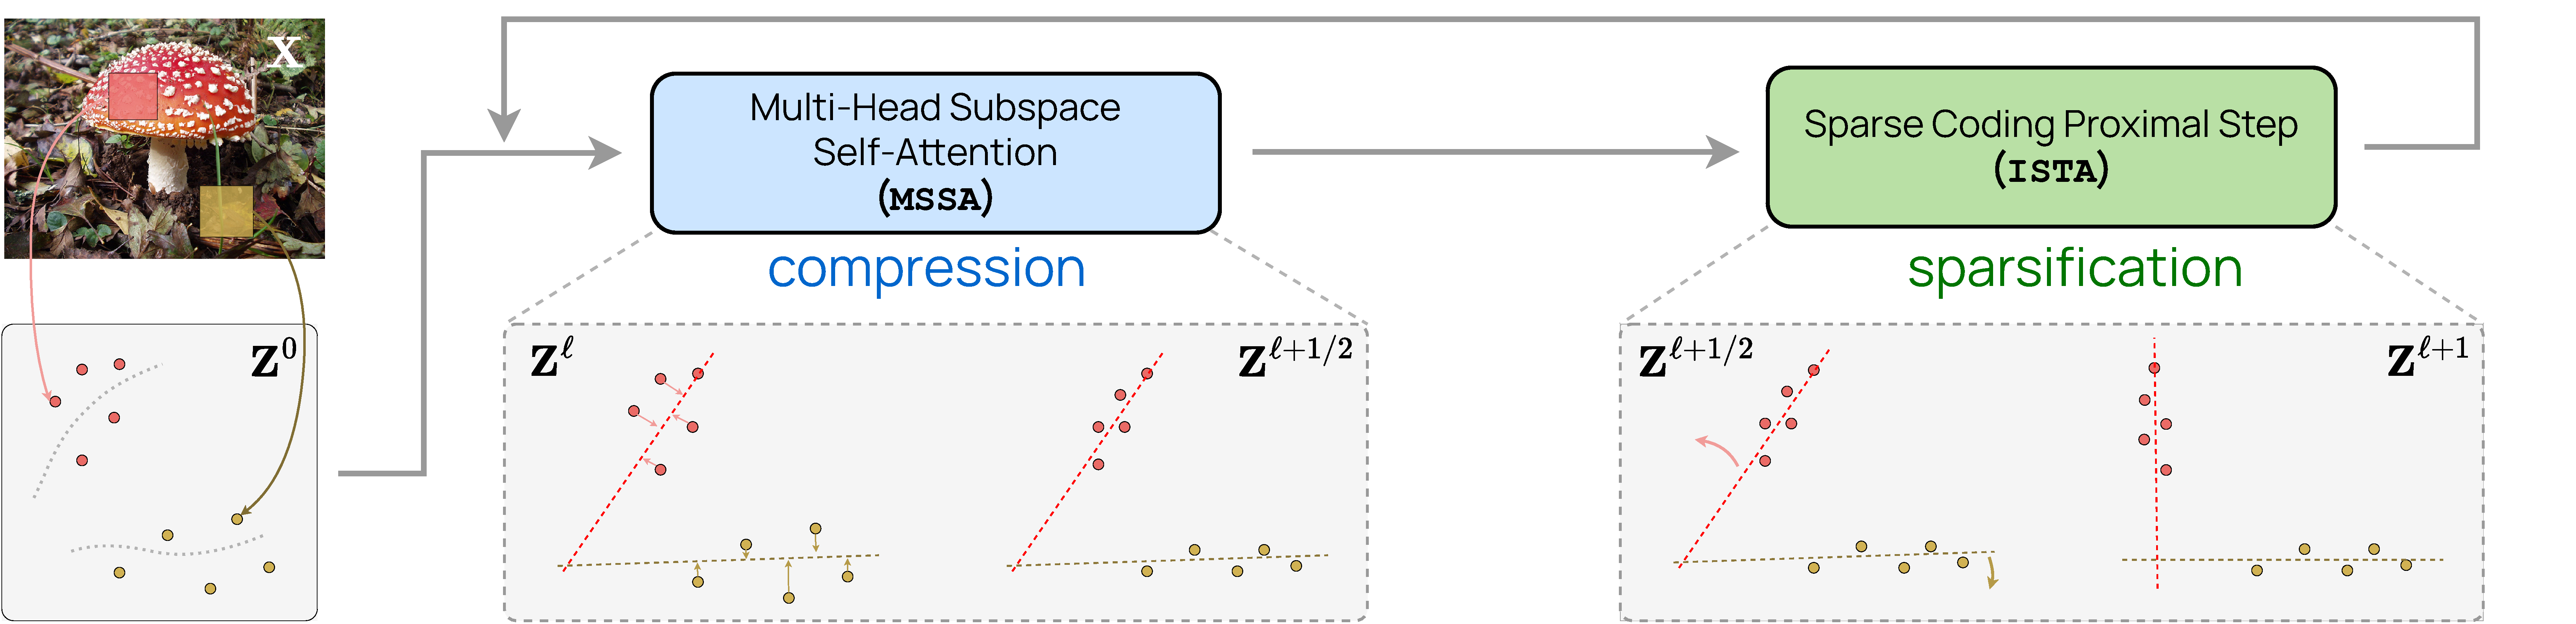
\includegraphics[width=\textwidth]{figs_chap4/CRATE_fig1_patches.pdf}
     \vspace{-0.1in}
     \caption{
     \textbf{\textsc{crate} 白盒深度网络设计的“主循环”。}
     在将输入数据编码为令牌序列 $\vZ^0$ 后,\textsc{crate} 构建一个深度网络,通过连续的{\textit{\textbf{压缩}}}(针对分布的局部模型,生成 $\vZ^{\ell+1/2}$)和{\textit{\textbf{稀疏化}}}(针对全局字典,生成 $\vZ^{\ell+1}$),将数据转换为低维子空间的规范配置。
     重复堆叠这些块并通过反向传播训练模型参数,可以得到一个强大且可解释的数据表示。
     }
        \label{fig:crate-diagram}
\end{figure}

% \begin{figure}
%      \centering
%      \includegraphics[width=0.99\textwidth]{figs_chap4/crate_compression_sparsification.pdf}
%      \caption{\small \textbf{CRATE 白盒深度网络设计的“主循环”。} 在将输入数据 \(\vX\) 预处理成令牌序列 \(\vZ^1\) 后,CRATE 构建一个深度网络,通过连续的{\color{blue!60!black}\bf\textit{压缩}}(针对分布的局部模型,生成 $\vZ^{\ell+1/2}$)和{\color{green!60!black}\bf\textit{稀疏化}}(针对全局字典,生成 $\vZ^{\ell+1}$),将数据转换为低维子空间的规范配置。重复堆叠这些块并通过反向传播训练模型参数,可以得到一个强大且可解释的数据表示。
%         }
%         \label{fig:encoder_compression_sparsification}
% \end{figure}

\begin{remark}[\textbf{前向传播和反向传播的角色}]\label{sub:forward_backward}
    与其他展开优化方法(如 ReduNet \cite{chan2021redunet})相比,我们\textit{显式地建模}每一层 $\vZ^\ell$ 和 $\vZ^{\ell + 1/2}$ 的分布,可以是通过线性子空间的混合,也可以是从字典中稀疏生成。我们引入的解释是,在每一层 \(\ell\),学习到的子空间基 \(\vU_{[K]}^{\ell}\) 和学习到的字典 \(\vD^{\ell}\) 共同充当一个\textit{码本}或\textit{分析滤波器},对每一层 \(\ell\) 的中间表示进行编码和转换。由于第 \(\ell\) 层的输入分布首先由 \(\vU_{[K]}^{\ell}\) 建模,然后由 \(\vD^{\ell}\) 转换,因此每一层的输入分布是不同的,所以我们需要在每一层使用一个单独的码本来获得最简约的编码。这些码本的参数(即子空间基和字典),之前假设是完全已知的,实际上是从数据中学习的(例如,通过端到端训练中的\textit{反向传播})。

    因此,我们的方法在概念上清晰地分离了前向“优化”和后向“学习”,对于如此推导出的白盒深度神经网络。也就是说,在其前向传播中,我们将每一层解释为一个算子,它在给定一个学习到的模型(即一个码本)的情况下,将其输入的分布转换为一个更简约的表示。在其反向传播中,这个模型的码本,即每一层输入的分布,被更新以更好地拟合某个(监督的)输入-输出关系,如图 \ref{fig:forward-backward} 所示。这种概念上的解释意味着模型表示对特定任务和损失具有一定的不可知性;特别是,许多类型的任务和损失都将确保每一层的模型得到拟合,这保证了模型能产生简约的表示。
\end{remark}




% \yima{用图来说明前向和后向传播的作用...}

% \yima{一个例子,演示 CRATE 在像 CIFAR10 这样的简单数据集上如何工作?}
% \yaodong{添加了 CRATE 在 ImageNet-1k 上的结果。}

我们现在通过在 ImageNet-1K 上的 top-1 分类准确率以及在几个广泛使用的下游数据集上的迁移学习性能,来展示所提出的网络 \textsc{crate} 的经验性能。
我们在表 \ref{tab:crate_comparison_with_sota} 中总结了结果。迁移学习的方法是使用交叉熵损失进行微调,并从预训练的网络初始化。
由于设计的白盒 Transformer 架构在注意力块 (\texttt{MSSA}) 和非线性块 (\texttt{ISTA}) 中都利用了参数共享,\textsc{crate}{-Base} 模型 (2280 万)
的参数数量与 ViT-Small (2205 万)~\cite{dosovitskiy2020image} 相似,并且少于同样配置的 ViT-Base (8654 万) 参数的 30%。
从表 \ref{tab:crate_comparison_with_sota} 中,我们发现,在模型参数数量相似的情况下,我们提出的网络在 ImageNet-1K 和迁移学习性能上与 ViT 相当,同时具有简单且有原则的设计。此外,在相同的训练超参数下,我们观察到 \textsc{crate} 具有良好的扩展行为——我们通过扩大模型规模持续提高性能。总而言之,\textsc{crate} 通过直接实现我们的原则性架构,在现实世界的大规模数据集上取得了有希望的性能。我们将在最后的应用章节 \ref{ch:applications} 中提供更多关于图像分类实验结果的实现细节和分析。

\begin{figure}[t]
    \begin{subfigure}[t]{0.48\textwidth}
        \centering
        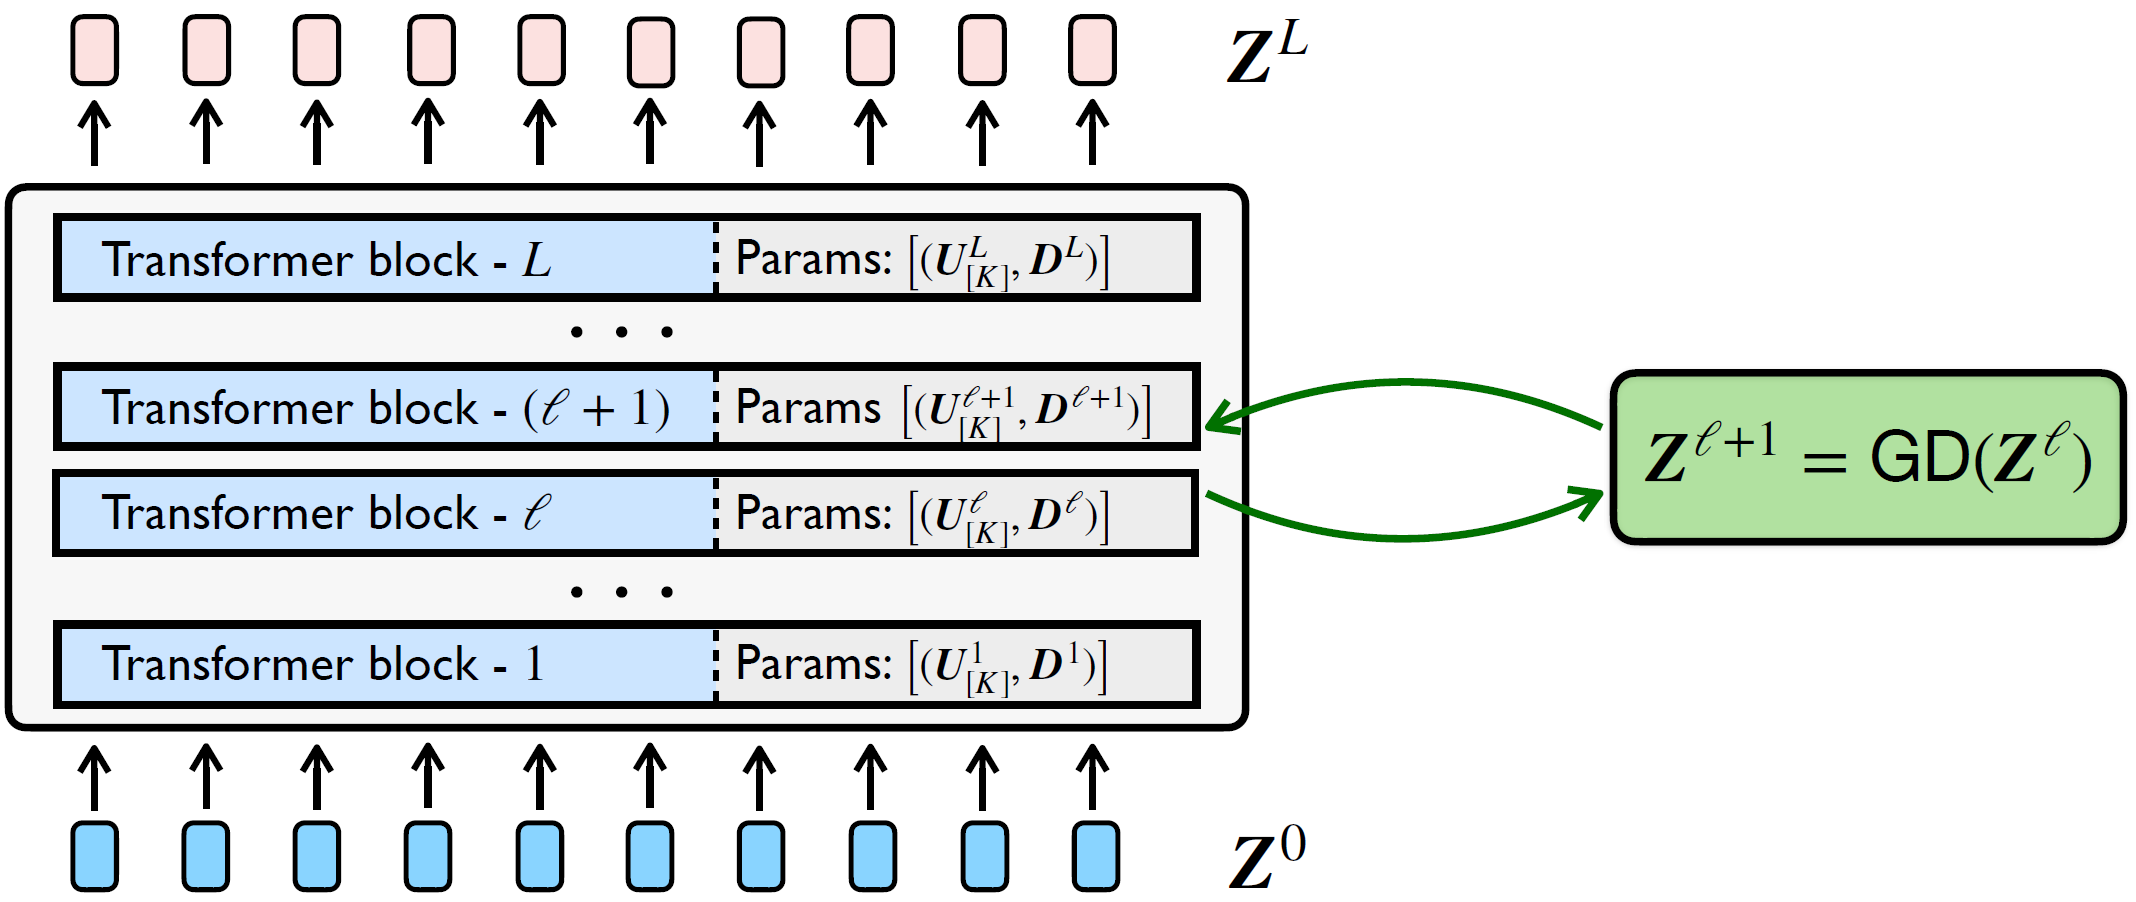
\includegraphics[width=\textwidth]{figs_chap4/forward.png}
        \caption{\bf 前向传播}
    \end{subfigure}
    \hfill
    \begin{subfigure}[t]{0.48\textwidth}
        \centering
        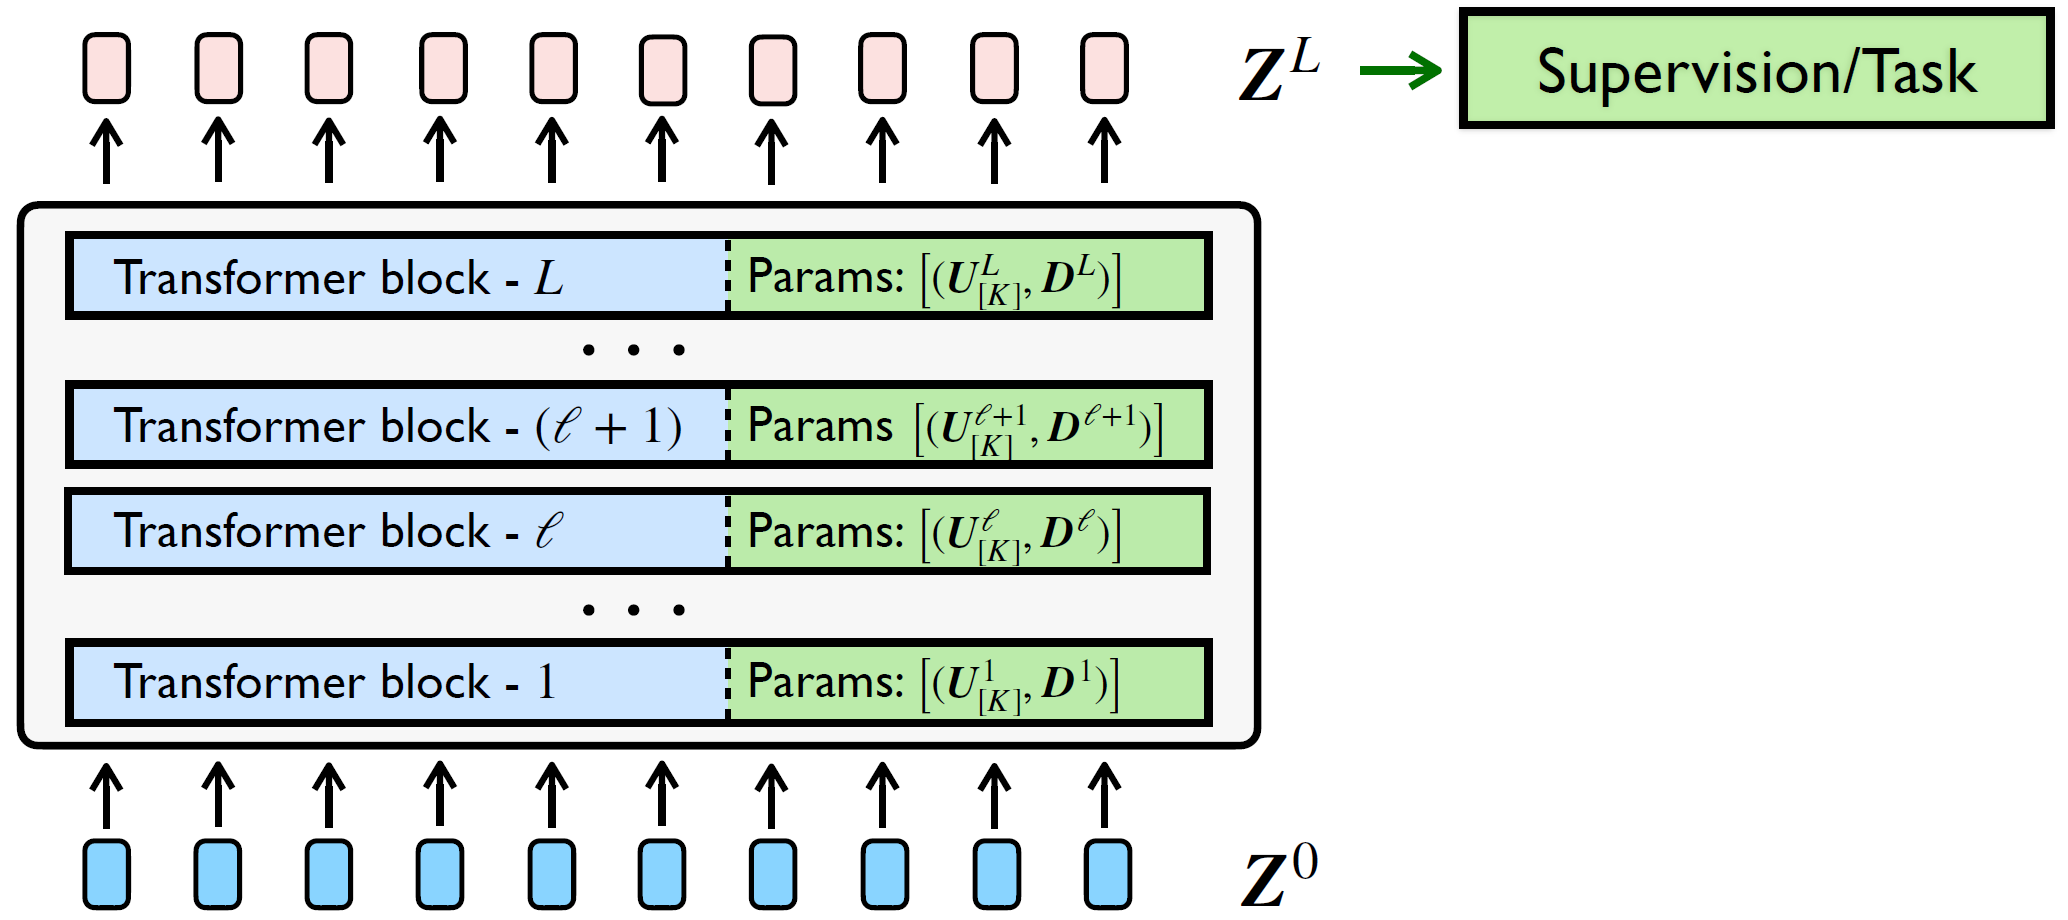
\includegraphics[width=\textwidth]{figs_chap4/backward.png}
        \caption{\bf 反向传播}
    \end{subfigure}
    \caption{\small {\bf 深度网络中前向传播和反向传播的角色}。(a) 给定固定的子空间和字典 $\{(\bm U_{[K]}^{\ell}, \bm D^{\ell})\}_{\ell=1}^L$,每一层在前向传播中对表示进行压缩和稀疏化;(b) 反向传播从训练数据中学习子空间和字典 $\{(\bm U_{[K]}^{\ell}, \bm D^{\ell})\}_{\ell=1}^L$。}
    \label{fig:forward-backward}
\end{figure}


\begin{table*}[t!]
\centering
\caption{\small \textsc{crate} 在不同模型规模下,在 ImageNet-1K 上预训练后,在各种数据集上的 Top-1 分类准确率。对于 ImageNet-1K/ImageNet-1K ReaL,我们直接评估 top-1 准确率。对于其他数据集,我们使用在 ImageNet 上预训练的模型作为初始化,并通过微调评估迁移学习性能。}
\label{tab:crate_comparison_with_sota}
\small
    \setlength{\tabcolsep}{13.6pt}
\resizebox{0.98\textwidth}{!}{\begin{tabular}{@{}lcccc|cc@{}}
\toprule
\textbf{模型} & \textsc{crate}{-T}  &  \textsc{crate}{-S} & \textsc{crate}{-B} & \textsc{crate}{-L} & { \color{gray} ViT-T} &  { \color{gray}ViT-S } \\
\midrule
\midrule
 \# 参数 & 6.09M & 13.12M & 22.80M & 77.64M & { \color{gray} 5.72M} & { \color{gray} 22.05M} \\
\midrule
 ImageNet-1K & 66.7 & 69.2 & 70.8 & 71.3 & { \color{gray} 71.5} & { \color{gray} 72.4} \\
 ImageNet-1K ReaL & 74.0 & 76.0 & 76.5 & 77.4 & { \color{gray} 78.3 } & { \color{gray} 78.4} \\
 \midrule
 CIFAR10 & 95.5 & 96.0 & 96.8 & 97.2 & { \color{gray} 96.6} & { \color{gray} 97.2} \\
 CIFAR100 & 78.9 & 81.0 & 82.7 & 83.6 & { \color{gray} 81.8} & { \color{gray} 83.2}\\
 Oxford Flowers-102 & 84.6 & 87.1 & 88.7 & 88.3 & { \color{gray} 85.1} & { \color{gray} 88.5}\\
 Oxford-IIIT-Pets & 81.4 & 84.9 & 85.3 & 87.4 & { \color{gray} 88.5} & { \color{gray} 88.6} \\
 \bottomrule
\end{tabular}}
\end{table*}



\section{按设计衍生的深度架构变体} \label{sec:chap4-derive-white-box-transformer-variants}

到目前为止,我们希望我们已经提供了令人信服的证据,表明(流行的)深度网络的作用是实现某些优化算法,以最小化学习表示的编码率(或最大化信息增益)。然而,熟悉优化方法的读者可能已经注意到,上述架构(ReduNet 或 CRATE)对应于相当基础的优化技术。它们在效率或有效性方面可能有很大的改进空间。此外,如果我们相信所提出的用于解释深度网络的理论框架是正确的,它不仅应该帮助解释现有架构,还应该指导我们开发更高效和有效的架构。在本节中,我们将展示情况确实如此:由此产生的新架构不仅完全可解释,而且具有保证的正确性和更高的效率。

% \pw{CRATE 网络的新变体,更高效或更有效;添加更多评论}

% \yaodong{待办事项:在这个白盒架构框架下,我们可以从原则出发设计新的架构,而不是通过试错。这里我们展示了 CRATE 的两种替代设计。}



\subsection{纯注意力 Transformer 架构} \label{sub:aot}

在本小节中,我们提出了一个极简的 Transformer 架构,它由基于 MSSA 算子的可解释层组成。为了推导出一个只包含必要组件的完全可解释的 Transformer 架构,
我们主张表示学习的目标是将一组带噪声的初始令牌表示压缩到一个低维子空间的混合模型中。% 为了压缩这些带噪声的令牌表示,相关的去噪操作自然地呈现为 MSSA 算子的形式(见 \eqref{eq:Multi-Head-SSA})。通过将这种迭代去噪操作展开成一个深度网络,我们得到了一个高度紧凑的架构,它在每一层只包含自注意力算子和跳跃连接。
这里,我们假设初始令牌表示 $\bm Z^{(1)}$ 是从一个混合的低秩高斯分布中采样得到的,并受到噪声扰动,如下所示:
\begin{definition}\label{def:MoG}
令 $C_1,\dots,C_K$ 为索引集 $[N]$ 的一个划分,$\bm U_k \in \mathcal{O}^{d \times p_k}$ 表示第 $k$ 个子空间的正交基,对于每个 $k \in [K]$。我们说令牌表示 $\{\bm z_i \}_{i=1}^N \subseteq \R^d$ 是从一个带噪声的低秩高斯分布混合中采样的,如果对于每个 $k \in [K]$,
\begin{align}\label{eq:MoG}
    \bm z_i = \underbrace{\bm U_{k} \bm a_i}_{\bf 信号} + \underbrace{\sum_{j \neq k}^K \bm U_j \bm e_{i,j}}_{\bf 噪声},\ \forall i \in C_k,
\end{align}
其中 $\bm{a}_i \overset{i.i.d.}{\sim} \mathcal{N}(\bm{0},\bm{I}_{p_k})$ 且 $\bm{e}_{i,j} \overset{i.i.d.}{\sim} \mathcal{N}(\bm{0},\delta^2\bm{I}_{p_j})$ 对于所有 $i \in C_k$ 和 $k \in [K]$,$\{\bm{a}_i\}$ 和 $\{\bm{e}_{i,j}\}$ 分别是相互独立的,并且 $\{\bm{a}_i\}$ 独立于 $\{\bm{e}_{i,j}\}$。
\end{definition}
该模型作为一个理想化的框架,用于近似现实世界预训练 LLM 中的令牌表示。它假设令牌表示是从多个带噪声的低秩高斯分布的混合中采样的。在此模型下,表示学习的目标是将一组带噪声的初始令牌表示压缩到相应的子空间中。此外,该模型与关于预训练大型语言模型中令牌表示结构的两个公认假设非常吻合:“线性表示假说” \citep{jiang2024origins,park2023linear} 和“叠加假说” \citep{elhage2022toy,yun2021transformer}。

\begin{remark}
    线性表示假说认为,LLM 中的令牌表示位于编码语义特征的低维线性子空间中。类似地,叠加假说提出,这些表示可以近似地表示为这些特征向量的稀疏线性组合。在 \Cref{def:MoG} 中,子空间的每个基 $\bm U_k$ 可以被解释为一组语义特征,其中每个特征对应于令牌含义的特定方面。然后,令牌表示近似地表示为这些子空间基的稀疏线性组合,捕获令牌的基本语义成分,同时忽略不相关的维度。
\end{remark}

\paragraph{令牌表示的去噪算子。} 现在,我们证明 MSSA 算子(见 \eqref{eq:Multi-Head-SSA})可以增量地对从上述模型生成的令牌表示进行去噪。具体来说,我们考虑对于每个 $\ell =1 ,\dots,L$,
\begin{align}\label{eq:MSSA}
    \bm Z^{(\ell+1)} =  \bm Z^{(\ell)} + \eta \sum_{k=1}^K \bm U_k\bm U_k^T \bm Z^{(\ell)} \varphi \left(\bm Z^{(\ell)^T}\bm U_k\bm U_k^T\bm Z^{(\ell)} \right),
\end{align}
其中 $\{\bm U_k\}_{k=1}^K$ 在 \Cref{def:MoG} 中定义,$\eta > 0$ 是步长,$\varphi$ 是一个逐元素操作的算子,例如 soft-max、ReLU 或其他函数。为了简化我们的推导,我们假设 \Cref{def:MoG} 中的子空间是相互正交的,即对于所有 $k \neq j$,$\bm U_k^T\bm U_j = \bm 0$。请注意,这个假设并不具有限制性,因为在高维空间中,随机的低维子空间以高概率相互不相干,即 $\bm U_k^T\bm U_j \approx \bm 0$ \citep{Wright-Ma-2021}。\footnote{人们可以很直接地将我们的结果推广到非正交子空间,只需进行稍微复杂的分析。}

\begin{figure}[t]
    \begin{subfigure}[t]{0.45\textwidth}
        \centering
        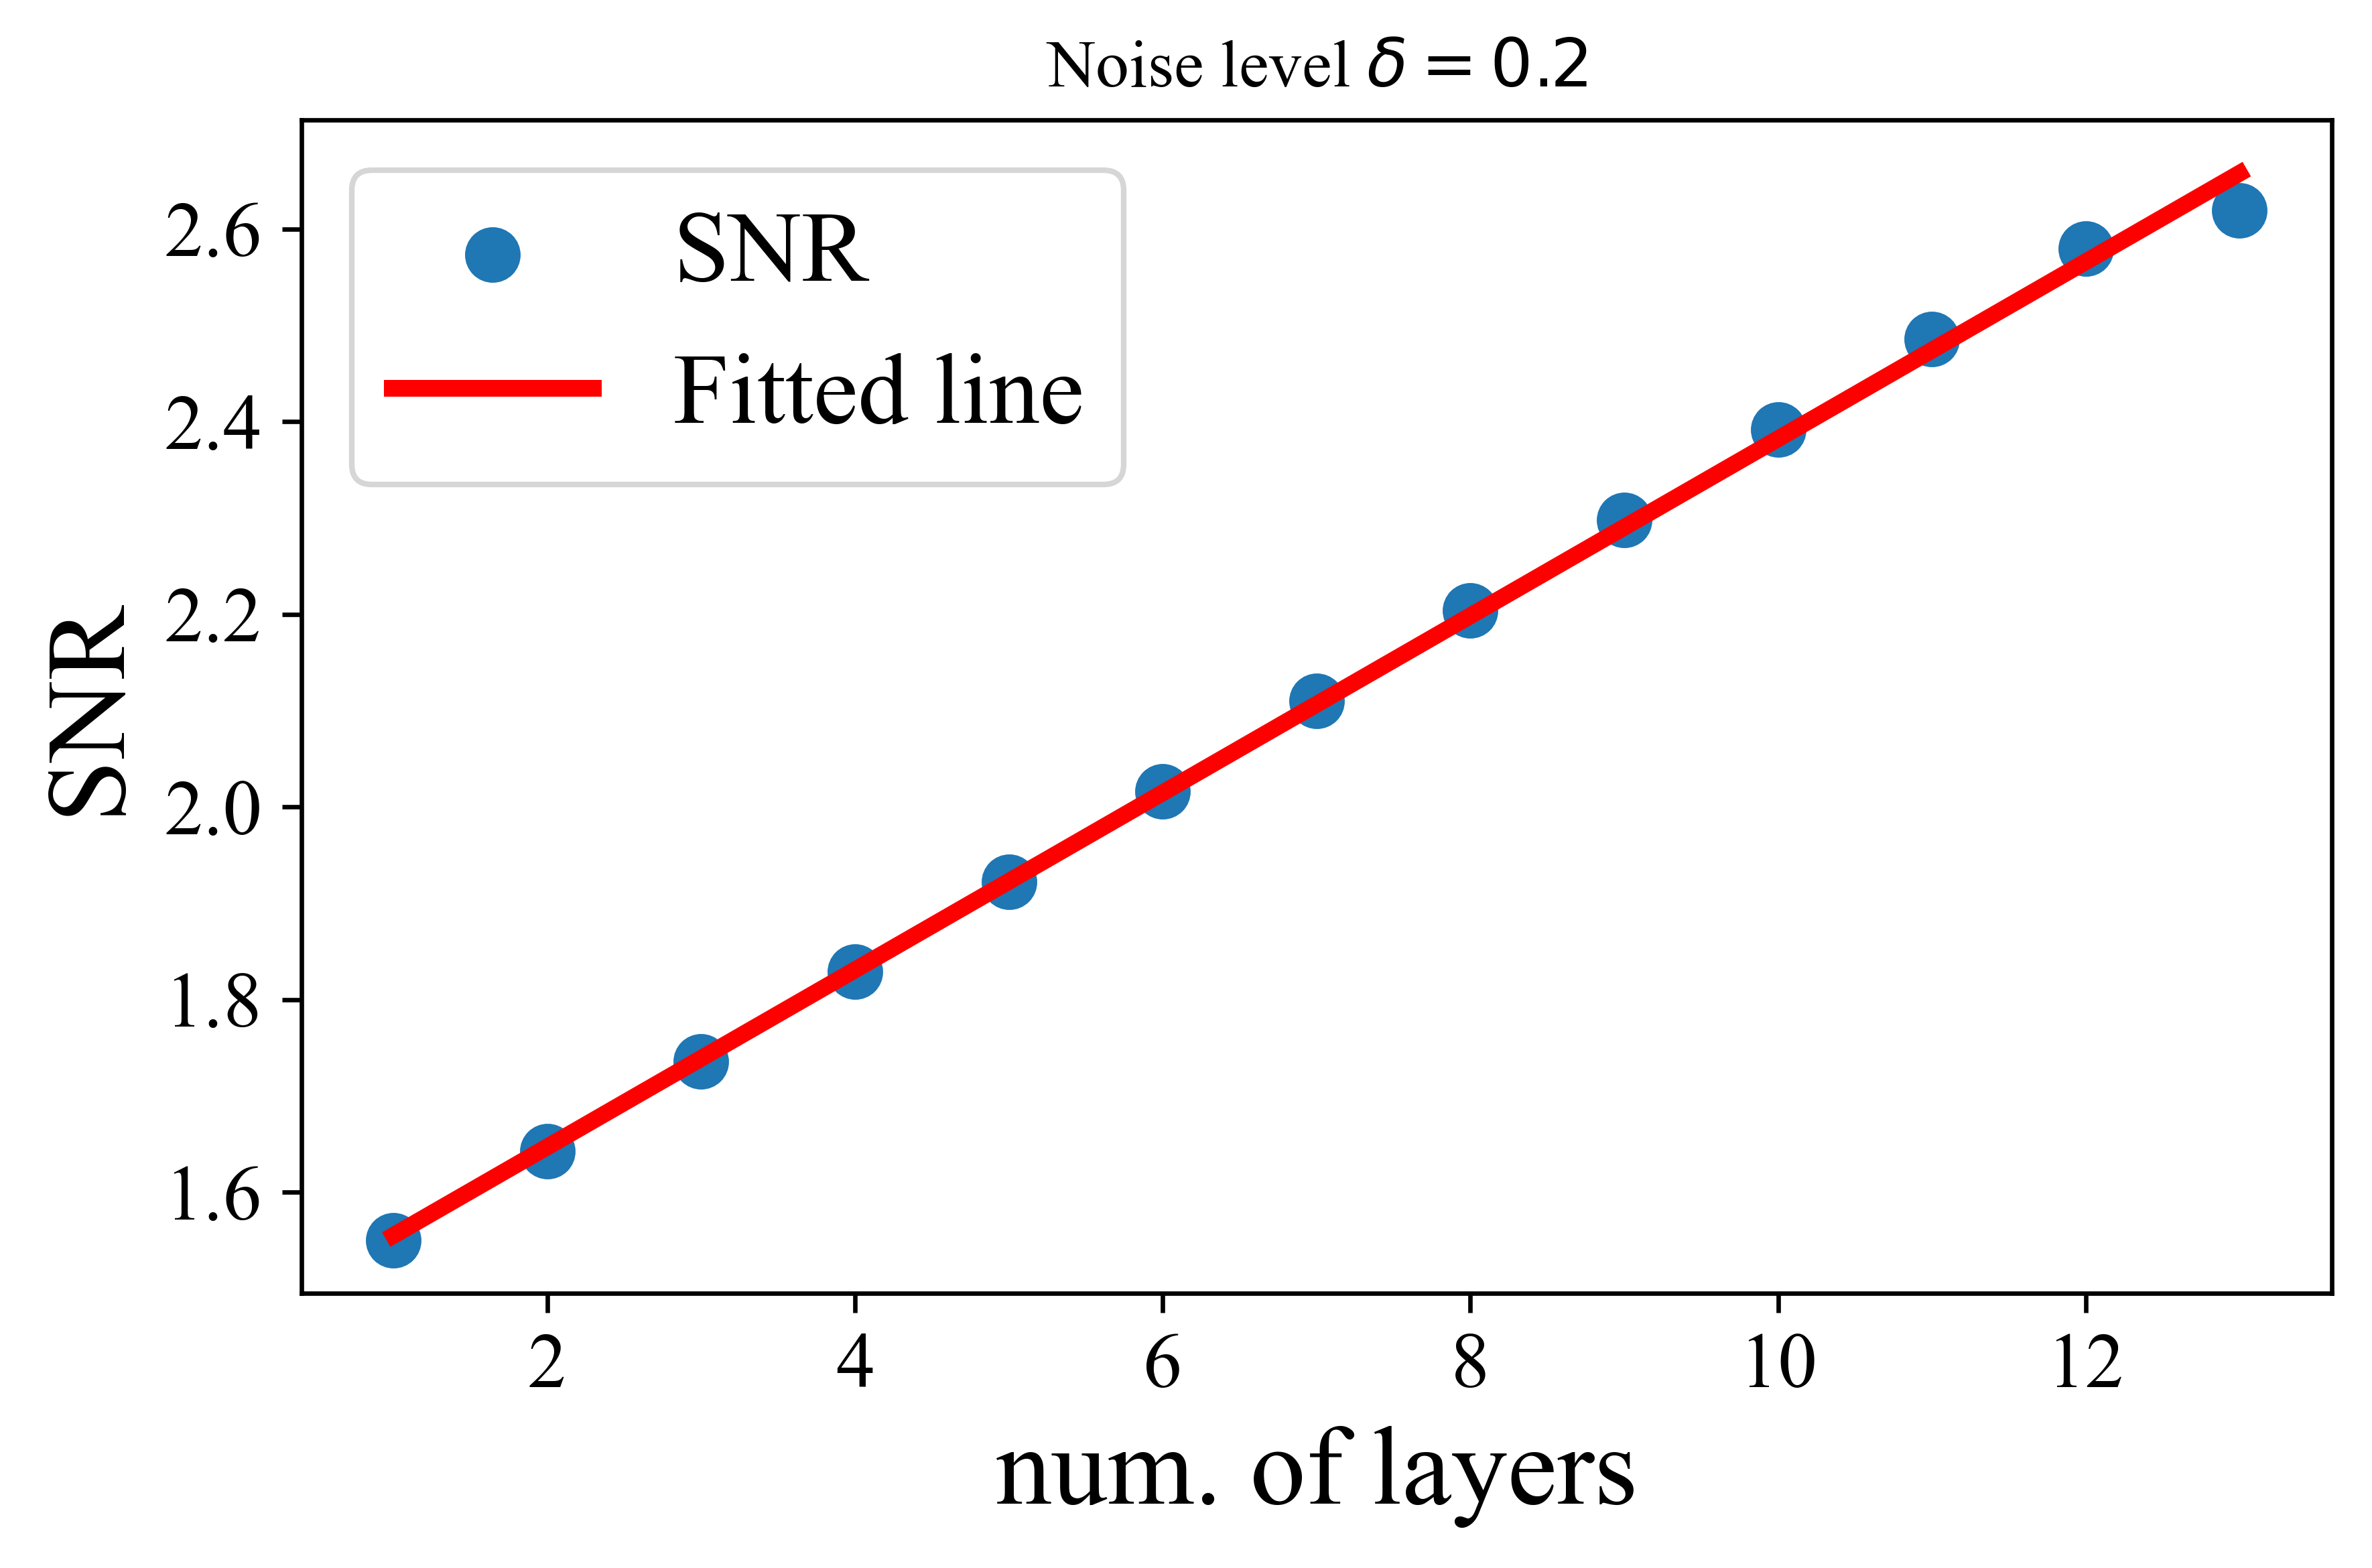
\includegraphics[width=\textwidth]{figs_chap4/SNR1.png}
        \caption{噪声水平 $\delta = 0.2$}
    \end{subfigure}
    \hfill
    \begin{subfigure}[t]{0.45\textwidth}
        \centering
        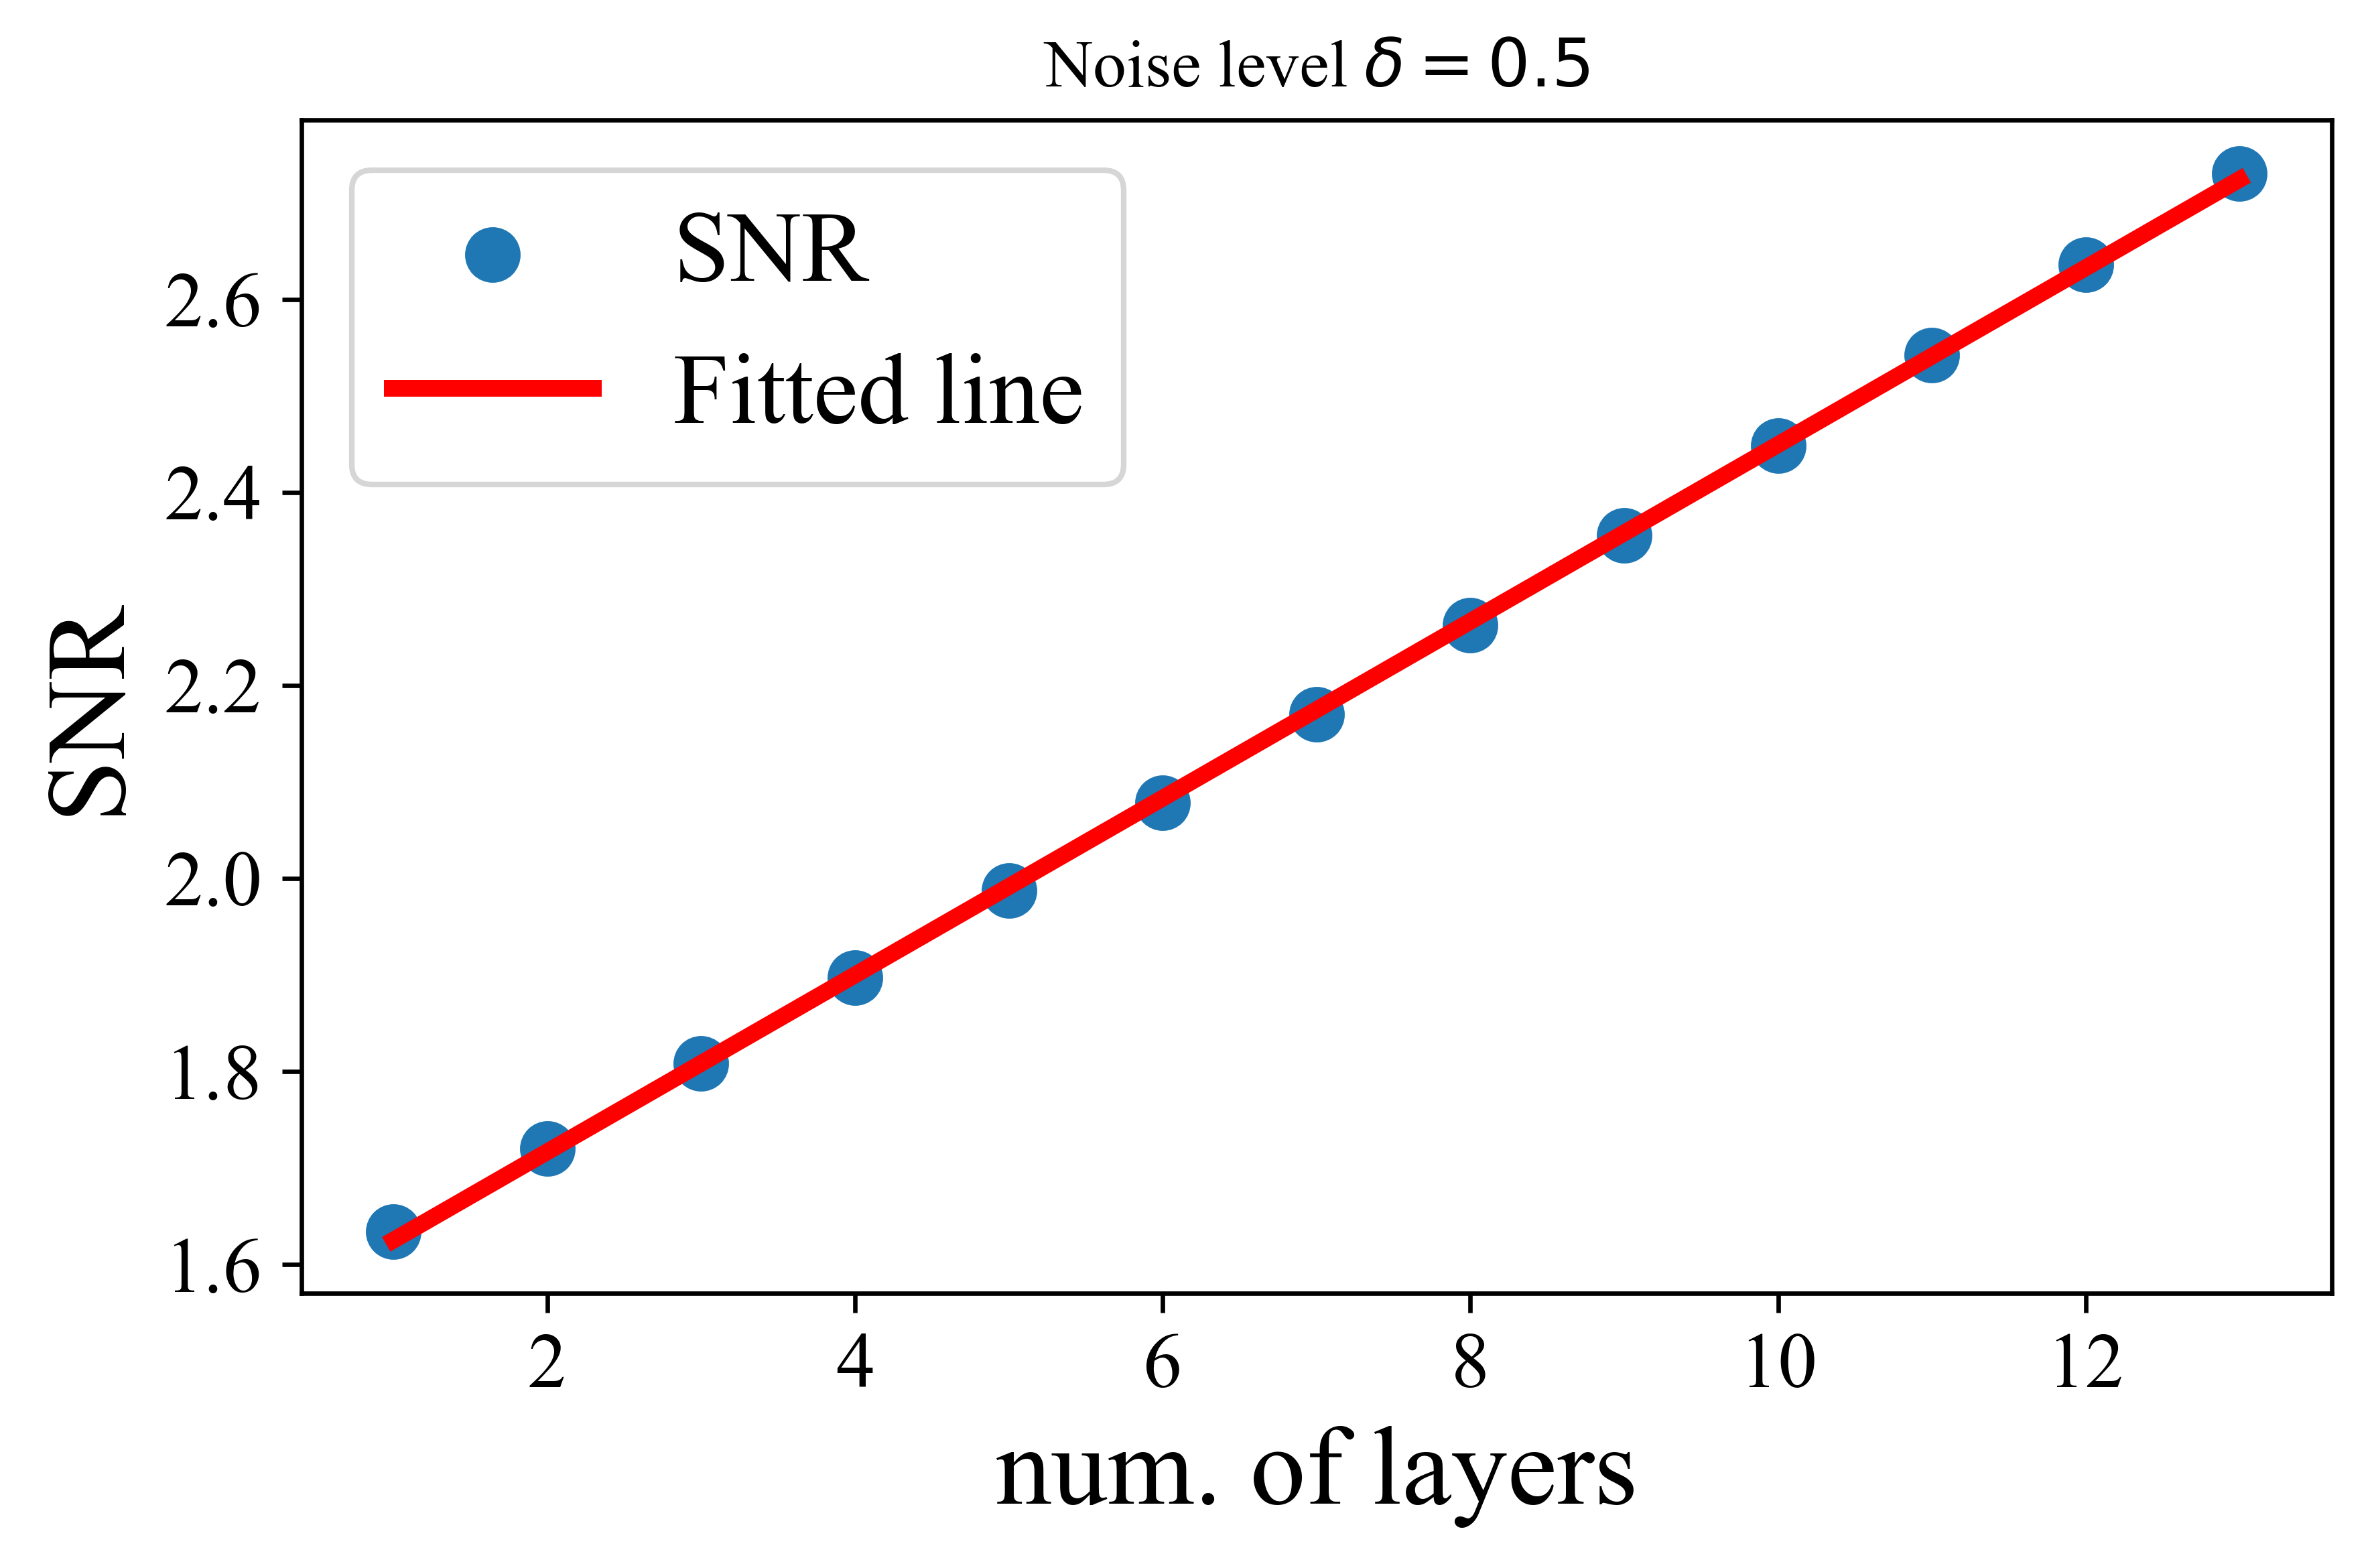
\includegraphics[width=\textwidth]{figs_chap4/SNR2.png}
        \caption{噪声水平 $\delta = 0.5$}
    \end{subfigure}
    \caption{{\bf 纯注意力 Transformer 的去噪性能。} 在这里,我们从 \Cref{def:MoG} 中的低秩高斯混合模型中采样初始令牌表示。然后,我们应用 (\ref{eq:MSSA}) 来更新令牌表示,并报告每一层的信噪比。}  \label{fig:MSSA}
\end{figure}


现在,令 $\bm Z_k^{(\ell)}$ 的列表示第 $\ell$ 层来自第 $k$ 个子空间的令牌表示。为了量化去噪能力,我们定义第 $\ell$ 层令牌表示的每个块的信噪比(SNR)如下:
\begin{align}\label{def:SNR}
\mathrm{SNR}(\bm Z_k^{(\ell)}) :=  \frac{\|\bm U_k\bm U_k^T\bm Z_k^{(\ell)} \|_F}{\|(\bm I - \bm U_k\bm U_k^T)\bm Z_k^{(\ell)} \|_F},\quad \forall k \in [K].
\end{align}
为了简化我们的分析,我们假设 $p=p_1=\dots=p_K$, $N_1=\dots=N_K=N/K$,并且
\begin{align}\label{eq:orth}
\begin{bmatrix}
\bm U_1 & \dots & \bm U_K
\end{bmatrix} \in \mathcal{O}^{d\times Kp}.
\end{align}

基于上述设置,我们现在描述 MSSA 算子的去噪性能。

\begin{figure*}[t]
\begin{center}
        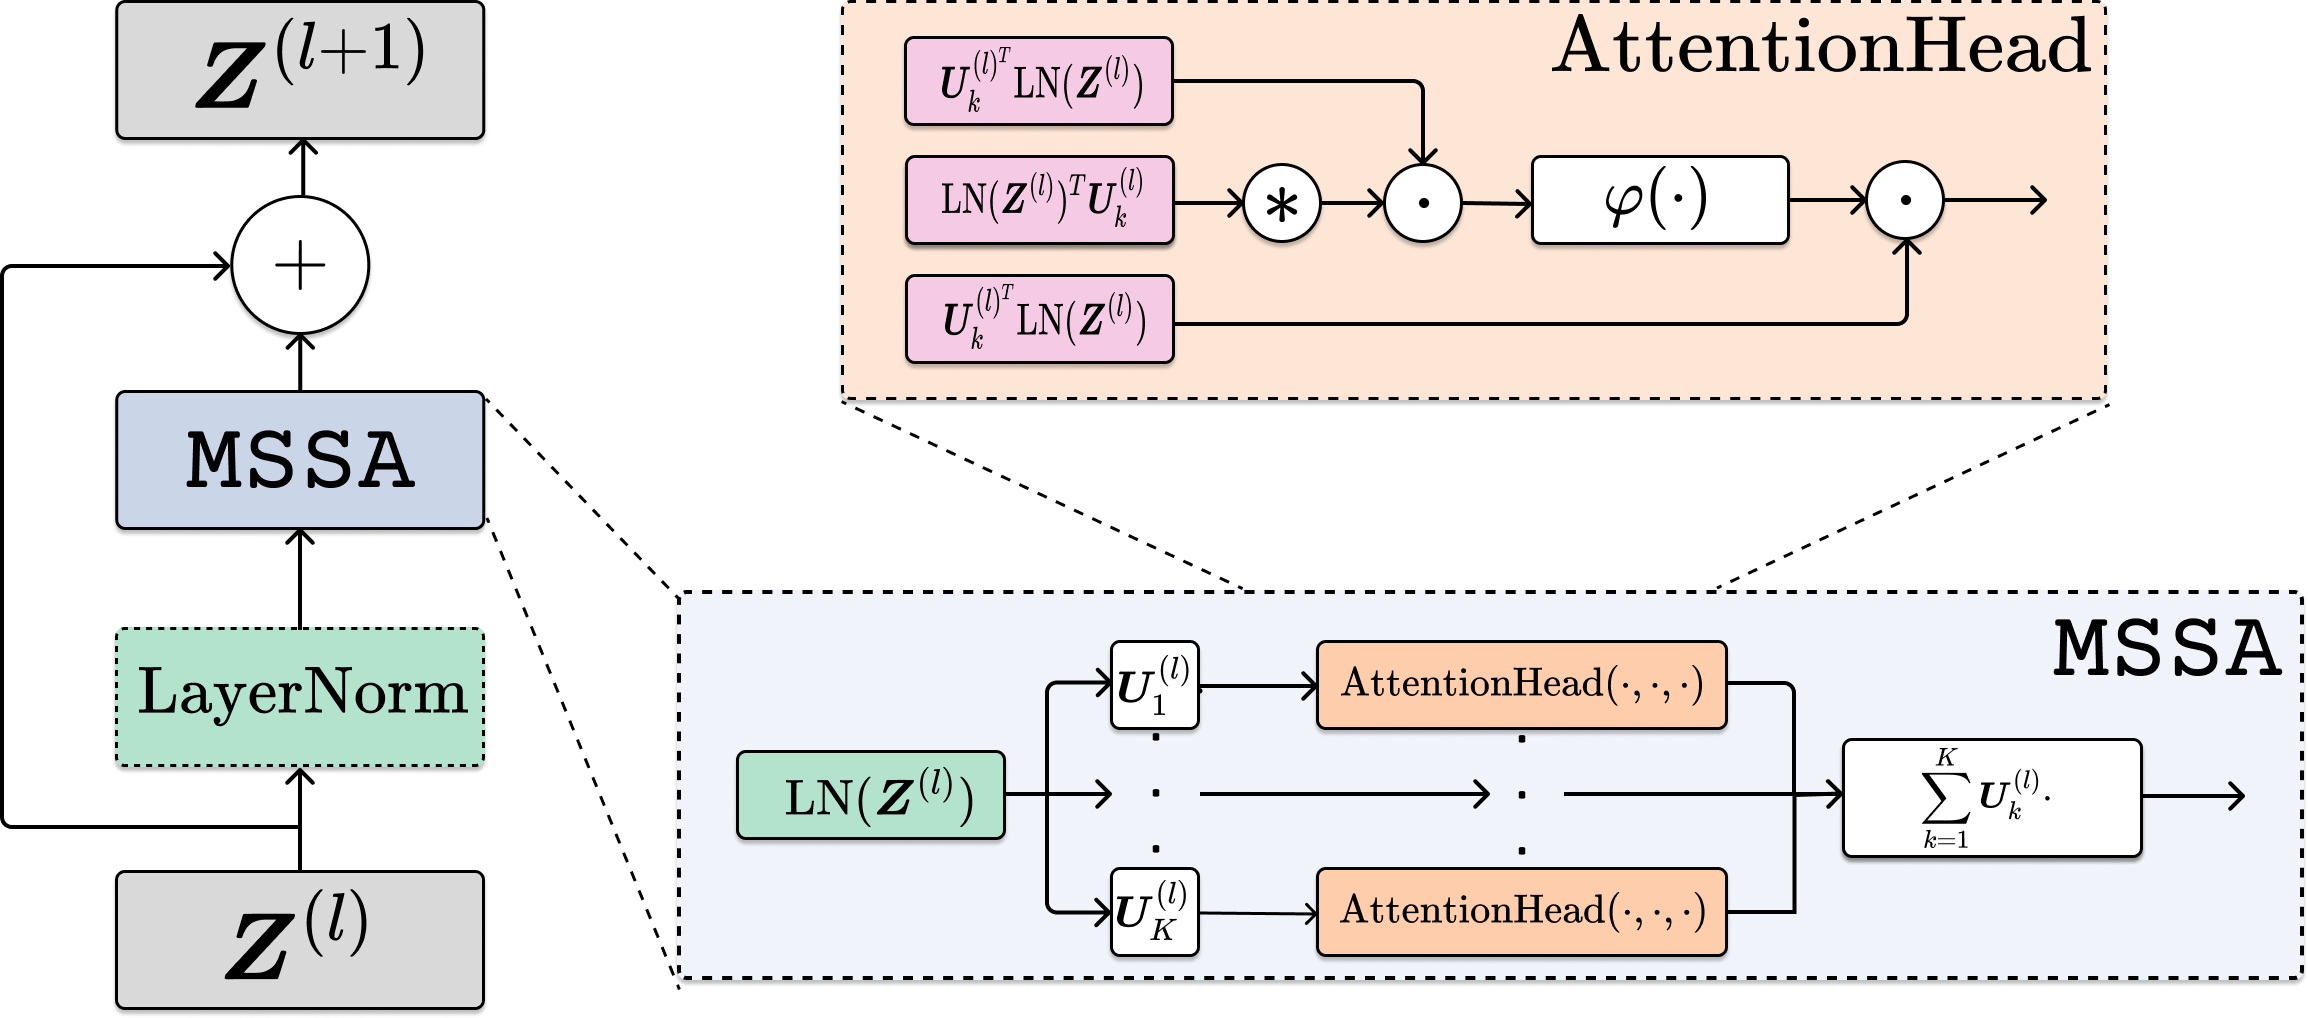
\includegraphics[width=0.75\textwidth]{figs_chap4/MSSA.png}
    \caption{\textbf{纯注意力 Transformer 架构的细节。} 每一层由 MSSA 算子和一个跳跃连接组成。此外,仅在语言任务中包含 LayeNorm。在实践中,应用反向传播来使用训练样本训练模型参数。 % \qq{这个图太大了}
    }\label{fig:transformer}
\end{center}
\end{figure*}

\begin{theorem}\label{thm:1}
令 $\bm Z^{(1)}$ 在 \Cref{def:MoG} 中定义,且公式 (\ref{eq:MSSA}) 中的 $\varphi(\cdot)$ 为
%\begin{align}\label{eq:relu}
$\varphi(\bm x) = h\left(\sigma(\bm x)\right)$,
%\end{align}
其中 $\sigma:\R^N \to \R^N$ 是 soft-max 函数, $h:\R^N \to \R^N$ 是一个逐元素的阈值函数,对于每个 $i \in [N]$,$h(x) = \tau \mathbb{I}\left\{x > \tau\right\}$。假设 $p \gtrsim \log N$,$\delta \lesssim \sqrt{\log N}/\sqrt{p}$,并且
\begin{align*}
\tau \in \left( \frac{1}{2},  \frac{1}{1+N\exp(-9p/32)} \right].
\end{align*}
对于足够大的 $N$,以至少 $1-KLN^{-\Omega(1)}$ 的概率,对于每个 $\ell \in [L]$,下式成立:
    \begin{align}\label{eq:SNR}
        \mathrm{SNR}(\bm Z_k^{(\ell+1)}) = (1+\eta\tau) \mathrm{SNR}(\bm Z_k^{(\ell)}),\ \forall k \in [K].
    \end{align}
\end{theorem}
该定理表明,当初始令牌表示是从噪声水平为 $O(\sqrt{\log N}/\sqrt{p})$ 的低秩高斯分布混合中采样时,我们证明了所提出的 Transformer 的每一层都以线性速率对令牌表示进行去噪。这表明 MSSA 算子在各层之间减少噪声的效率。值得注意的是,我们的理论结果得到了 \Cref{fig:MSSA} 中实验观察的有力支持。该定理为通过展开 (\ref{eq:MSSA}) 推导出的 Transformer 架构的实际去噪能力提供了理论基础。

\begin{remark}
    在这个模型下,表示学习的目标是将一组带噪声的初始令牌表示压缩到相应的子空间中。然而,我们应该指出,在现实世界的应用中,令牌表示展现出更复杂的结构,表示学习的目标是通过压缩令牌集来找到一个紧凑和结构化的表示。
\end{remark}


\paragraph{纯注意力 Transformer。} 现在,我们正式提出一个纯注意力的 Transformer 架构。具体来说,通过将迭代优化步骤 (\ref{eq:MSSA}) 展开为深度网络的层,我们构建了 \Cref{fig:transformer} 中的 Transformer 架构。所提出的架构的每一层仅由 MSSA 算子和一个跳跃连接组成。对于语言任务,我们还在 MSSA 算子之前额外加入了 LayerNorm 以提高性能。完整的架构是通过堆叠这些层,以及必要的任务特定预处理和后处理步骤(如位置编码、令牌嵌入和最终的任务特定头)来构建的,以适应不同的应用。




总的来说,标准的仅解码器 Transformer 架构由以下关键组件组成 \cite{vaswani2017attention}:(1) 位置编码,(2) 多头 QKV 自注意力机制,(3) 前馈 MLP 网络,(4) 层归一化,以及 (5) 残差连接。相比之下,我们提出的 Transformer 架构通过引入几个关键的简化,采用了流线型设计。具体来说,它采用了共享 QKV 的子空间自注意力机制,排除了 MLP 层,并减少了 LayerNorm 的使用频率。

%\yima{这种架构的理论保证。}

% \paragraph{去噪性能的理论保证。}

% 为了研究纯注意力 Transformer 的去噪性能,我们假设初始令牌表示 $\bm Z^{(0)}=[\bm z_1^{(0)},\dots,\bm z_N^{(0)}]$ 是从一个带噪声的低秩高斯分布混合中抽取的,如下所示。







\subsection{线性时间注意力:令牌统计 Transformer}\label{sub:tost}

在本小节中,我们基于编码率缩减目标,提出了一种新的 Transformer 注意力算子,其计算复杂度与令牌数量成线性关系。具体来说,我们推导了 MCR$^2$ 目标的一个新颖的变分形式,并表明从该变分目标的展开梯度下降得到的架构导出了一个名为令牌统计自注意力 (\texttt{TSSA}) 的新注意力模块。\texttt{TSSA} 具有{\em 线性的计算和内存复杂度},并从根本上不同于计算令牌之间成对相似度的典型注意力架构。回顾 \eqref{eq:MCR pi},$\bm \Pi = [\bm \pi_1, \ldots, \bm \pi_K] \in \R^{N \times K}$ 表示一个随机的“组分配”矩阵(即 $\bm \Pi \bm 1 = \bm 1$ 且 $\Pi_{ik} \geq 0, \  \forall (i,k) \in [N] \times [K]$),其中 $\Pi_{ik}$ 表示将第 $i$ 个令牌分配给第 $k$ 组的概率。

% 回顾一下,\(\X = [\x_{1}, \dots, \x_{N}] \in \R^{D \times N}\) 通常是一个矩阵值变量,Transformer 旨在找到一个\textit{表示映射},或者说一个从 \(\R^{D \times N}\) 到 \(\R^{d \times N}\) 的令牌映射 $f$,使得特征 $\Z = f(\X) = [\z_1, \ldots, \z_N] \in \R^{d \times N}$ 适合手头的任务。在 MCR$^2$ 中,令牌被假定属于一个包含 \(K\) 个组的底层集合,这些组可以(例如)代表令牌群体中的不同模式,MCR$^2$ 目标旨在找到每个组的令牌特征,这些特征在组内是\textit{压缩的},而所有令牌特征的集合则尽可能地扩展(见 \eqref{eq:MCR pi})。

%  特别地,令 $\bm \Pi = [\bm \pi_1, \ldots, \bm \pi_K] \in \R^{N \times K}$ 是一个随机的“组分配”矩阵(即 $\bm \Pi \bm 1 = \bm 1$ 且 $\Pi_{ik} \geq 0, \  \forall (i,k) \in [N] \times [K]$),它为每个令牌分配一个组成员概率(即 $\bm\Pi$ 的第 $i$ 行是第 $i$ 个令牌的组成员概率向量)。然后,令 $\epsilon > 0$ 且 $N_k \doteq \langle \bm\pi_k, \bm 1 \rangle$ 对于每个 \(k \in [K]\),MCR$^2$ 目标,记为 $\Delta R(\bm Z,\bm \Pi)$,是:
% \begin{equation}
%     \label{eq:mcr2}
%     \Delta R(\Z,\bm\Pi) \doteq \underbrace{\frac{1}{2} \log \det \left( \I + \frac{d}{\epsilon^{2}} \frac{1}{N} \Z \Z^{\top} \right)}_{\doteq R(\Z)} - \underbrace{\frac{1}{2} \sum_{k=1}^{K} \frac{N_{k}}{N} \log \det \left( \I + \frac{d}{\epsilon^{2}} \frac{1}{N_k}\Z \mathrm{Diag}(\bm \pi_k) \Z^{\top} \right) }_{\doteq R_{c}(\Z, \bm\Pi)}.
% \end{equation}

\paragraph{编码率的新变分形式。} 首先,我们考虑基于矩阵谱的凹函数的一般形式的 MCR$^2$ 类目标。也就是说,对于一个给定的 PSD 矩阵 $\bm M \in \PSD(d)$ 和任何标量 $c \geq 0$,我们有 $\log \det (\I + c \bm M) = \sum_{i=1}^{d} \log( 1 + c \lambda_i(\bm M))$,其中 $\lambda_i (\bm M)$ 是 $\bm M$ 的第 $i$ 大特征值。此外,请注意 $\log(1 + c \sigma)$ 是 $\sigma$ 的一个凹非减函数。因此,我们用一种更一般的 MCR$^2$ 形式来描述我们的结果,该形式基于 PSD 矩阵的一般谱函数,形式为 $F(\bm M) = \sum_{i=1}^{d} f(\lambda_i(\bm M))$,其中 $f$ 是凹且非减的。特别地,回顾我们上面的讨论,注意力机制源于 MCR$^2$ 压缩部分的展开,因此我们考虑一个更一般的 MCR$^2$ 风格的压缩函数:
\vspace{-2mm}
\begin{equation}
    R_{c,f}(\bm Z, \bm \Pi) \doteq \frac{1}{2}\sum_{k=1}^K \frac{N_k}{N} F\left( \frac{1}{N_k}\Z \mathrm{Diag}(\bm \pi_k) \Z^{\top} \right).
    \label{eq:mcr_c_gen}
\end{equation}



对于上述目标,我们现在注意到以下结果:
\begin{theorem}
\label{thm:var_concave}
    令 \(f \colon [0, \infty) \to \R\) 为非减、凹函数,且满足 \(f(0) = 0\),并令 \(F \colon \PSD(d) \to \R\) 的形式为 \(F(\bm M) = \sum_{i = 1}^{d}f(\lambda_{i}(\bm M))\)。则对于每个 \(\bm M \in \PSD(d)\) 和 \(\bm Q \in \O(d)\),我们有
    \begin{equation}
        \label{eq:U_bound}
        F(\bm M) \leq  \sum_{i=1}^{d} f\left( (\bm Q^{\top} \bm M \bm Q)_{ii} \right).
    \end{equation}
    此外,\eqref{eq:U_bound} 中的不等式在任何对角化 $\bm M$ 的 $\bm Q$ 下都取等号,如果 $f$ 是严格凹的,则 \eqref{eq:U_bound} 中的不等式取等号的条件是\textit{当且仅当} $\bm Q$ 对角化 $\bm M$。
\end{theorem}

利用上述结果,我们可以用一个等价的变分目标替换 \eqref{eq:mcr_c_gen},其形式为
\vspace{-2mm}
\begin{equation}
    \label{eq:var_comp}
    R^{\rm var}_{c,f} (\Z,\bm \Pi \mid \bm U_{[K]}) \doteq \frac{1}{2}\sum_{k=1}^K \frac{N_k}{N} \sum_{i=1}^{d} f\left(\frac{1}{N_k} (\bm U_{k}^{\top} \Z \mathrm{Diag}(\bm \pi_k) \bm Z^{\top} \bm U_{k})_{ii} \right),
\end{equation}
这里的等价性是指,对于 \Cref{thm:var_concave} 中描述的最优 $\{ \bm U_k \in \O(d)\}_{k=1}^K$ 矩阵选择(即对角化每个 $\Z \mathrm{Diag}(\bm \pi_k) \Z^\top $ 的正交矩阵),我们将得到一个紧界,使得 $ R^{\rm var}_{c,f} (\Z,\bm \Pi \mid \bm U_{[K]}) = R_{c,f} (\Z,\bm \Pi)$。请注意,通常情况下,要达到这个界限,需要为每个 $\Z$ 的采样实例选择一个新的最优 $\bm U_{k}$ 参数集,以对角化每个 $\Z\mathrm{Diag}(\bm \pi_{k})\Z^{\top}$,这对于网络架构来说显然是不切实际的。
作为一种替代观点,我们不是将数据($\Z$)视为固定的,并试图优化 $\bm U_k$ 参数以达到紧的变分界,而是可以采用上面描述的算法展开设计原则,设计一个算子来扰动 $\Z$,以增量地最小化 $R_{c, f}^{\rm var}(\cdot \mid \bm U_{[K]})$。为了明确这一点,每个变分界在 $\Z \mathrm{Diag}(\bm \pi_k) \Z^\top$ 的特征空间与 $\bm U_k$ 的列对齐时变得紧密,因此通过旋转 $\Z$ 的适当列(即对应于 $\bm \pi_k$ 中大值的列)以与 $\bm U_k$ 对齐,我们可以接近一个紧的变分界。也就是说,我们不是旋转 $\bm U_k$ 以与每个 $\Z$ 实例的数据对齐,而是可以旋转每个 $\Z$ 中的令牌特征以与 $\bm U_k$ 对齐。

遵循这种方法,我们计算 $R_{c,f}^{\rm var}$ 关于 $\Z$ 的梯度下降步骤。
为了开始这个计算,首先令 $\bm \pi \in \Re^N$ 为任何逐元素非负的向量。那么我们有
\begin{equation}\label{eq1:grad Rcf}
\nabla_{\Z} \ \frac{1}{2} \sum_{i = 1}^{d} f(  (\Z \mathrm{Diag}(\bm \pi) \Z^{\top} )_{ii}) %&
%\; \Diag \left( \nabla f\left[ \diag(\Z \Diag(\p) \Z^{\top}) \right] \right) \Z  \Diag(\p) \\
= \; \mathrm{Diag}(\nabla f[ \Z^{\odot 2} \bm \pi] ) \Z \mathrm{Diag}(\bm \pi),
\end{equation}
%
%其中 $\Z^{\odot 2}$ 表示将 $\Z$ 逐元素二次幂(即 $(\Z^{\odot 2})_{ij} = Z_{ij}^2$),$\nabla f[\cdot]$ 表示将 $f(x)$ 关于 $x$ 的梯度逐元素应用于向量。
其中 $\nabla f$ 是 $f$ 的梯度,并且(回顾一下)$\nabla f[\cdot]$ 将 $\nabla f$ 应用于括号中向量的每个元素。特别地,对于 $ f(x) = \log(1 + (d/\epsilon^{2}) x)$,$\nabla f(x) = (d / \epsilon^{2}) (1+ (d / \epsilon^{2}) x)^{-1}$ 只是一个非线性激活函数。另外,(回顾一下)$N_{k} = \langle \bm \pi_{k}, \bm 1\rangle$。因此,$R^{\rm var}_{c,f}$ 关于 $\Z$ 的梯度是:
\begin{align}\label{eq2:grad Rcf}
    \nabla_{\Z} R^{\rm var}_{c,f}(\Z,\bm \Pi \mid \bm U_{[K]}) =  \frac{1}{n} \sum_{k=1}^K \bm U_{k} \underbrace{\mathrm{Diag} \left( \nabla f\left[ (\bm U_{k}^{\top} \Z)^{\odot 2}  \frac{\bm \pi_k}{\langle \bm \pi_{k}, \bm 1\rangle} \right] \right)}_{\doteq \bm D(\Z, \bm \pi_{k} \mid \bm U_{k})} \bm U_{k}^{\top} \Z \mathrm{Diag}(\bm \pi_k).
\end{align}
(注意,常数 $1/N$ 来自于求和中每一项的 $(N_{k}/N)\cdot (1/N_{k}) = 1/N$ 常数。)如果我们现在考虑关于第 $j$ 个令牌 $\z_j$ 的梯度步骤,我们就能得到我们提出的增量压缩算子,即我们对\textit{自注意力} + 残差算子的替代:
%
\vspace{-2mm}
\begin{equation}\label{eq:layer-operation-orig}
    \z_j^+ = \z_{j} - \tau \nabla_{\z_{j}}R_{c, f}^{\rm var}(\Z, \bm \Pi \mid \bm U_{[K]}) = \z_j - \frac{\tau}{N} \sum_{k=1}^K \Pi_{jk} \bm U_{k} \bm D(\Z, \bm \pi_{k} \mid \bm U_{k}) \bm U_{k}^{\top} \z_j
\end{equation}
对于每个 \(j \in [n]\),其中 $\tau > 0$ 是增量优化的步长参数。然后,我们可以在 \Cref{fig:vcrate-architecture} 中构建一个 TOST 层。

\begin{figure}[t]
    \centering 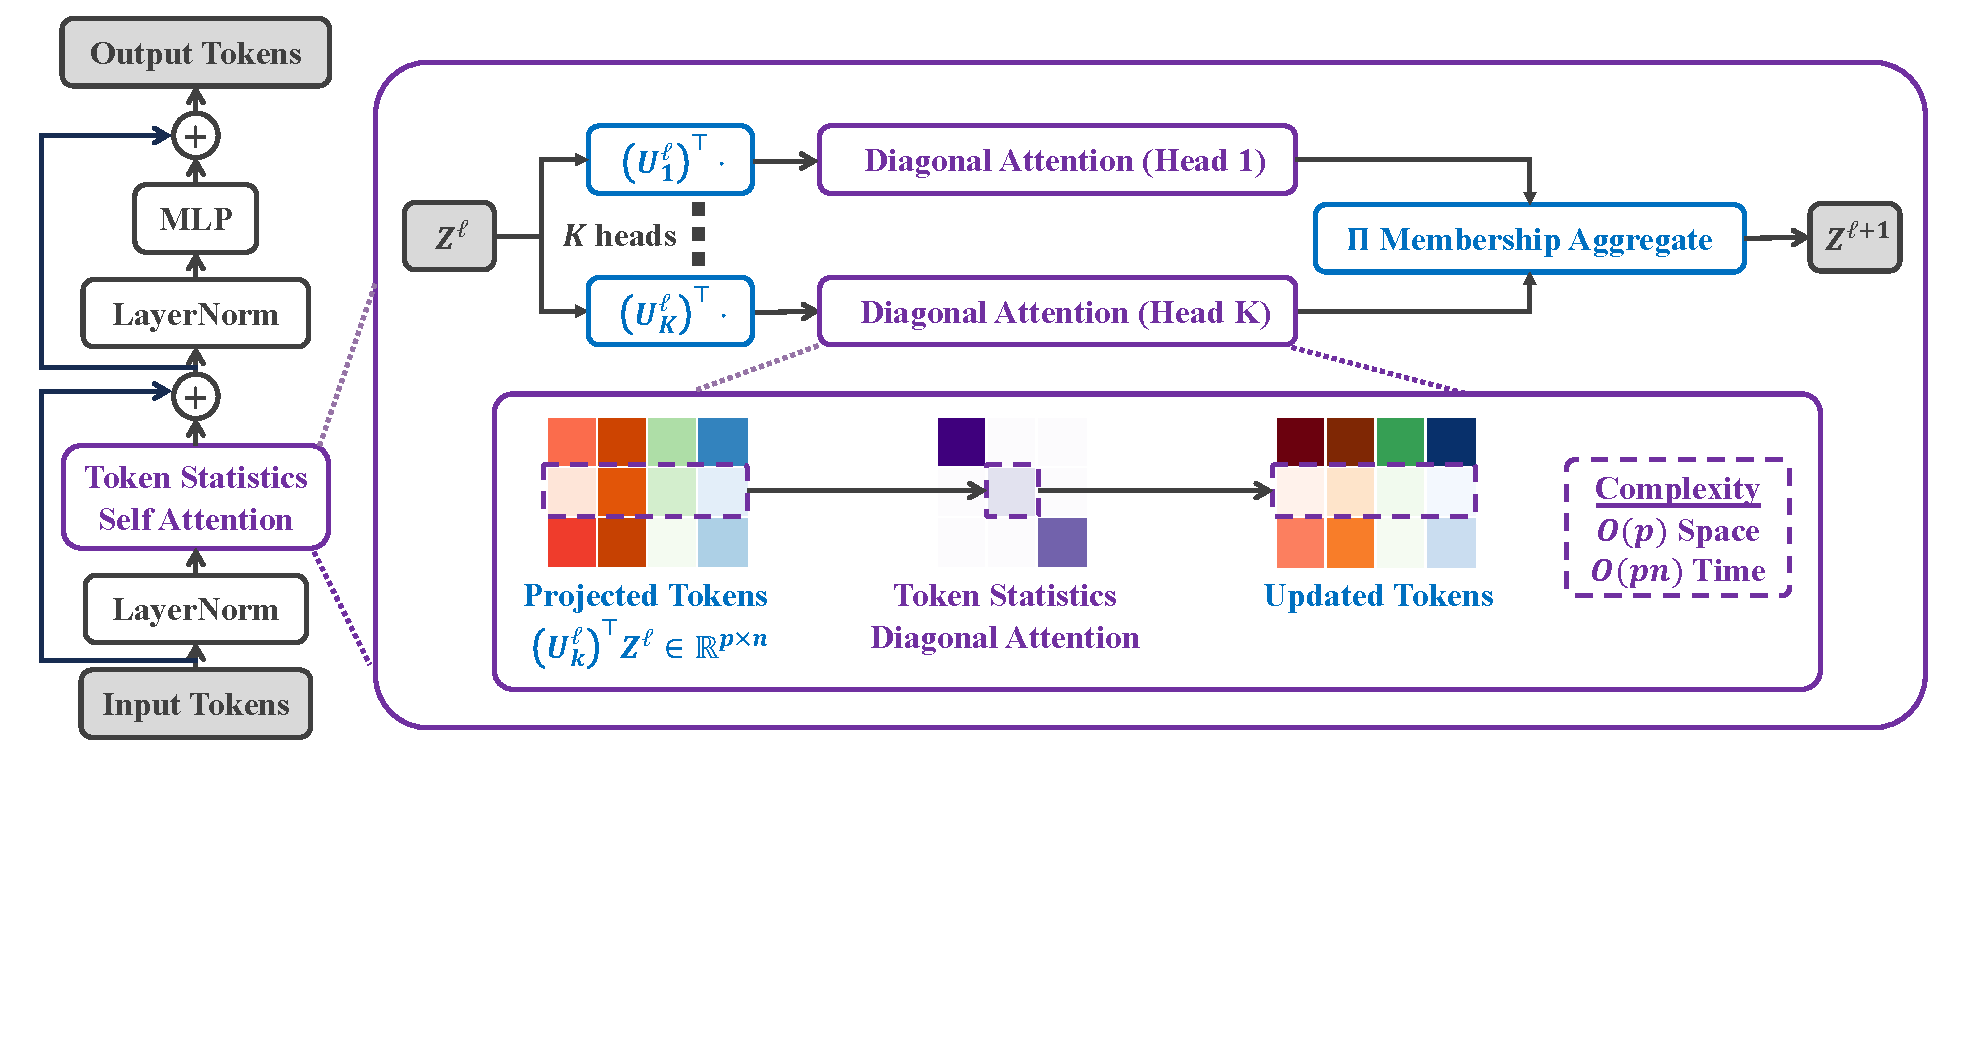
\includegraphics[width=1\textwidth,trim={0 5.0cm 0 0},clip]{figs_chap4/V-CRATE.pdf}
    \vspace{-1mm}
    \caption{\small \textbf{所提出的令牌统计 Transformer (ToST) 的一个层 $\ell$。} 值得注意的是,ToST 的自注意力通过将投影令牌的每一行\textit{仅乘以一个标量},从而高效地将令牌 $\Z^{\ell}$ 转换为 $\Z^{\ell+1}$。这降低了注意力的复杂度:其空间复杂度为 $O(p)$,时间复杂度为 $O(pn)$,其中 $p$ 是每个头的投影令牌的维度,n 是令牌的数量。
    }
    \label{fig:vcrate-architecture}
\end{figure}

\paragraph{模型解释。} 给定所提出的注意力算子 \eqref{eq:layer-operation-orig},首先回顾一下,$\bm\Pi$ 的行是非负的且和为 1
%(我们将在下一节讨论如何构建 $\P$)
,所以我们的算子取 $K$ 个“注意力头”式算子的加权平均,然后添加一个残差连接。利用 \(\sum_{k = 1}^{K}\Pi_{jk} = 1\),我们可以将 \eqref{eq:layer-operation-orig} 重写为: %可以等价地将我们的注意力算子重新表述为:
\vspace{-2mm}
\begin{equation}
\label{eq:z_up}
    \z_j^+ = \sum_{k=1}^K \Pi_{jk} \Big[ \z_j \underbrace{- \frac{\tau}{n} \bm U_{k} \bm D(\Z, \bm \pi_{k} \mid \bm U_{k}) \bm U_{k}^{\top}}_{\text{一个注意力头的动作}} \z_j \Big].
\end{equation}
也就是说,我们可以将每个注意力头看作是首先通过乘以 $\bm U_k^\top$ 将令牌特征投影到基 $\bm U_{k}$ 上,然后乘以对角矩阵 $\bm D(\Z, \bm \pi_{k} \mid \bm U_{k})$(简写为 \(\bm D_{k}\)),再通过乘以 $\bm U_{k}$ 投影回标准基,最后通过残差连接从原始令牌特征中减去这个结果。我们注意力层的核心是计算 $\bm D_{k}$。也就是说,\(\Pi_{jk} \geq 0\),所以 $\bm \pi_k / \langle \bm \pi_{k}, \bm 1\rangle \in \Re^N$ 构成了一个关于哪些令牌属于第 $k$ 组的概率分布。因此,$(\bm U^\top_k \Z)^{\odot 2} \bm \pi_k / \langle \bm \pi_{k}, \bm 1\rangle$ 估计了在由 $\bm \pi_k /  \langle \bm \pi_{k}, \bm 1\rangle$ 给出的分布下 $\bm U_k^\top \Z$ 的二阶矩。此外,由于 $f$ 是一个凹非减函数,$\nabla f(x)$ 随着 $x$ 的增加单调递减至 $0$,所以 $\bm D_{k}$ 的项(形式为 $\nabla f(x)$)在 $x=0$ 时达到最大值 %当 $x \approx 0$ 时接近 $\nabla f(0) > 0$
并随着 $x$ 的增加单调衰减至 $0$。

由此,我们得出了对我们的注意力头 + 残差算子 $[\I - (\tau/n)\bm U_{k}\bm D_{k}\bm U_{k}^{\top}]$ 的核心解释。也就是说,这个算子做了一个近似的低秩数据依赖投影,其中在投影 $\bm U_k^\top \Z$ 后具有大量“能量”的方向(即具有大二阶矩 $(\bm U_{k}^{\top}\Z)^{\odot 2}\bm \pi_k / \langle \bm \pi_{k}, \bm 1\rangle$ 的方向)被保留,而没有的则被抑制。要理解这一点,回顾一下 $\bm D_k$ 的项随着二阶矩的增加单调递减至 0,所以对于具有大二阶矩的方向,注意力 + 残差算子的作用很大程度上是恒等算子。相反,对于具有小二阶矩的方向,我们的算子减去沿这些方向的令牌投影,导致这些方向被抑制。与标准的自注意力算子相比,我们的方法显然不计算令牌之间的任何成对相似性。相反,$\Z$ 中令牌之间的相互作用仅通过它们对用于构建 $\bm D_{k}$ 的二阶矩统计量的贡献来影响算子。然而,与标准的自注意力算子类似,我们的方法仍然有一个清晰的解释,即执行一种朝向数据依赖的低秩结构的压缩,因为它执行了一个近似的低秩投影,其中被抑制的特定方向是那些与组中其他令牌没有强烈对齐的方向。

\paragraph{实际实现细节。} 在介绍了我们提出的注意力算子之后,我们现在讨论进一步的实际考虑。首先,到目前为止,我们一直避免讨论如何通过 $\bm\Pi$ 矩阵将令牌“分组”到各个注意力头中,但显然需要一种构建 $\bm\Pi$ 的方法来实现我们的方法。此外,我们在 \Cref{thm:var_concave} 中的变分形式要求 $\bm U$ 矩阵是方的和正交的,但理想情况下,人们希望使用更小的矩阵(即减少 $\bm U$ 中的列数)以提高效率,并放弃正交性约束。

在实践中,我们不强制执行正交性约束。为了减少 $\bm U$ 矩阵中的列数,我们注意到,与 CRATE \citep{yu2023white} 类似,如果我们假设组 \(k\) 内的特征 $\bm Z$(近似地)聚集在一个低维子空间周围——比如说维度为 \(p\)——那么组内-\(k\) 协方差 \(\Z\mathrm{Diag}(\bm \pi_{k})\Z^{\top}\) 是低秩的,其中回顾一下 \cite{yu2020learning} 表明 $\Z$ 的最优几何形状是每个组都是一个低秩子空间,与其他组正交。因此,我们可以明确地找到这个协方差的像的一个低维正交基,即组 \(k\) 中数据的线性张成。如果维度是 $p \leq d$,基可以由一个 $d\times p$ 的正交矩阵 $\bm U_k \in \O(d, p)$ 表示。在这种情况下,我们可以更有效地使用这些低秩正交基矩阵来上界 \(R_{c,f}\)。为了证明这一点,我们使用 \Cref{thm:var_concave} 的一个更通用的版本来得到以下推论。
\begin{corollary}\label{cor:var_concave_logdet}
    令 \(f \colon [0, \infty) \to \R\) 为非减、凹函数,且满足 \(f(0) = 0\),并令 \(F \colon \PSD(p) \to \R\) 的形式为 \(F(\bm M) = \sum_{i = 1}^{p}f(\lambda_{i}(\bm M))\)。令 \(\Z\)、\(\bm \Pi\) 固定。那么,对于所有 \(\bm U_{1}, \dots, \bm U_{K} \in \O(d, p)\) 使得对于所有 \(k \in [K]\),\(\mathrm{image}(\Z\diag(\bm \pi_{k})\Z^{\top}) \subset \mathrm{image}(\bm U_{k})\),我们有
    \begin{equation}
        R_{c, f}(\Z, \bm\Pi) \leq R_{c, f}^{\rm var}(\Z, \bm\Pi \mid \bm U_{[K]}),
    \end{equation}
     其中 \(R_{c, f}^{\rm var}\) 在 \eqref{eq:var_comp} 中正式定义。如果对于每个 \(k \in [K]\),\(\bm U_{k}\) 对角化 \(\Z\diag(\bm \pi_{k})\Z^{\top}\),则等式成立;如果 \(f\) 是强凹的,则此等式条件变为“当且仅当”。
\end{corollary}

定义我们的注意力算子的最后一步是估计组隶属度 $\bm\Pi$。为此,我们假设一个简单的模型,描述每个特征 \(\z_{j}\) 如何偏离其支撑子空间,然后找到最优的子空间分配。\cite{yu2023white} 表明,如果我们独立地将每个 \(\z_{j}\) 建模为属于一个低维高斯混合模型,其中每个高斯分布具有相同的谱,并支撑在以正交基 \(\bm U_{k}\) 为基础的子空间上,再加上协方差为 \(\eta \I\) 的独立高斯噪声,那么每个令牌 \(\z_{j}\) 属于每个子空间的后验概率由分配矩阵 \(\bm \Pi = \bm \Pi(\bm Z \mid \bm U_{[K]})\) 给出,如下所示:
\begin{align}\label{eq:pi}
    \bm \Pi = \begin{bmatrix} \boldsymbol{\nu}(\z_1 \mid \bm U_{[K]})^\top \\ \vdots \\ \boldsymbol{\nu}(\z_n \mid \bm U_{[K]})^\top \end{bmatrix}, \quad
\text{其中} \quad
\boldsymbol{\nu}(\z_j \mid \bm U_{[K]}) \doteq \operatorname{softmax}\left( \frac{1}{2\eta} \begin{bmatrix} \|  \bm U_{1}^{\top} \z_j \|_2^2 \\ \vdots \\ \| \bm U_{K}^{\top} \z_j \|_2^2 \end{bmatrix} \right), \quad \forall j \in [n],
\end{align}
其中 $\eta$ 成为一个可学习的温度参数。因此,给定一个输入特征 \(\Z\),我们使用 \eqref{eq:pi} 估计 \(\bm\Pi\),然后计算注意力算子。将 \eqref{eq:pi} 中 \(\bm\Pi\) 的构造与
\eqref{eq:layer-operation-orig} 结合,我们得到了{\em 令牌统计自注意力}算子:
\begin{equation}
    \label{eq:tssa}
   \texttt{TSSA}(\Z \mid \bm U_{[K]}) \doteq -\frac{\tau}{n}\sum_{k = 1}^{K}\bm U_{k}\bm D(\Z, \bm\pi_{k} \mid \bm U_{k})\bm U_{k}^{\top}\Z\diag(\bm \pi_{k}),
\end{equation}
其中 \(\bm\pi_{k}\) 是在 \eqref{eq:pi} 中定义的 \(\bm\Pi = \bm\Pi(\Z \mid \bm U_{[K]})\) 的列,\(\bm D\) 在 \eqref{eq2:grad Rcf} 中定义。




\section{总结与注释}

%\yima{一个黑盒和白盒的比较表...}

% 随着深度学习的出现,经验设计的深度网络在捕捉复杂的非线性结构方面表现出了卓越的成功。诸如 CNN、RNN、LSTM、ResNet 和 Transformer 等架构已在各个领域得到广泛采用。然而,这些模型的设计在很大程度上是经验性的,由试错、消融研究和大规模超参数搜索驱动,对其内部工作原理的理论理解甚少。


本章介绍的材料基于关于该主题的一系列近期工作,包括 \cite{chan2021redunet, wang2024global, wang2025attention, wu2025token, yu2023white}。这些贡献涵盖了通过展开优化构建可解释深度网络的理论进展和实用方法。本章讨论的许多关键结果和证明直接源自或受这些基础工作的启发。


将优化算法展开以构建神经网络的想法可以追溯到开创性的工作 \cite{gregor2010learning}。在这项工作中,作者证明了稀疏编码算法——如迭代收缩阈值算法(ISTA)——可以展开形成多层感知器(MLP),有效地连接了迭代优化和神经网络设计。值得注意的是,\cite{monga2019algorithm} 证明了与通用网络相比,这种展开的网络更具可解释性、参数效率更高且更有效。在本章中,我们基于这一观点,通过展开旨在最小化有充分动机的目标——如前面介绍的(稀疏)率缩减目标——的优化算法,来开发有原则的、白盒的深度网络架构。这种方法不仅阐明了网络中每一层的作用,还为架构选择提供了理论基础,超越了经验试错,走向了可解释和目标驱动的设计。下面,我们将通过经验设计和启发式调整构建的传统 DNN 与我们基于数学基础的 ReduNet 架构进行比较:

\begin{center}
%\begin{small}
\begin{tabular}{| l || c | c |}
\hline
  & 传统 DNN & ReduNets\\ [0.5ex]
  \hline \hline
目标 & 输入/输出拟合 & 信息增益\\ [0.5ex]
  \hline
深度架构 & 试错法 & 迭代优化 \\  [0.5ex]
\hline
层算子 & 经验性的 & 投影梯度 \\  [0.5ex]
\hline
平移不变性 & CNN+数据增强 & 不变 ReduNets \\  [0.5ex]
\hline
初始化 & 随机/预设计 & 前向展开 \\ [0.5ex]
\hline
训练/微调 & 反向传播 & 前向/反向传播\\ [0.5ex]
\hline
可解释性 & 黑盒 & 白盒 \\ [0.5ex]
\hline
表示 & 隐藏/潜在 & 不相干子空间 \\ [0.5ex]
\hline
\end{tabular}
%\end{small}
\end{center}




\section{练习与扩展}


\begin{exercise}
    令 $\bm Z = [\bm Z_1,\dots,\bm Z_K] \in \R^{d\times m}$,其中对于每个 $k \in [K]$,$\bm Z_k \in \R^{d\times m_k}$。对于某个 $\alpha > 0$,令
    \begin{align*}
        R(\bm Z) = \log\det\left(\bm I + \alpha\bm Z\bm Z^T \right).
    \end{align*}
1. 给定任何方向 $\bm D \in \R^{d\times m}$,请证明 $\nabla R(\bm Z) = \alpha\bm X^{-1}\bm Z$ 且
    \begin{align*}
 \nabla^2 R(\bm Z)[\bm D, \bm D] =\alpha \mathrm{Tr}\left( \bm X^{-1}\bm D\bm D^T\right) - \frac{\alpha^2}{2}\mathrm{Tr}\left(\bm X^{-1}\left( \bm Z\bm D^T+\bm D\bm Z^T\right) \bm X^{-1}\left( \bm Z\bm D^T+\bm D\bm Z^T\right)\right),
    \end{align*}
    其中 $\bm X := \bm I + \alpha\bm Z\bm Z^T$。{\em 提示:} 注意
    \begin{align*}
        \nabla^2 R(\bm Z)[\bm D, \bm D] := \left\langle \lim_{t \to 0} \frac{\nabla R(\bm Z+ t\bm D) - \nabla R(\bm Z)}{t}, \bm D \right\rangle.
    \end{align*}

\noindent
2. 请证明
\begin{align*}
    R(\bm Z) \le \sum_{k=1}^K \log\det\left(\bm I + \alpha\bm Z_k\bm Z_k^T \right),
\end{align*}
其中等号成立当且仅当对于所有 $k \neq l \in [K]$,$\bm Z_k^T\bm Z_l = \bm 0$。
\medskip

\noindent
3. 给定某个 $\alpha >0$,令对于每个 $k \in [K]$,$\alpha_k=m\alpha/m_k$。请推导以下函数的一阶临界点的闭式解:
\begin{align*}
    f(\bm Z_k) = \frac{1}{2}\log\det\left(\bm I + \alpha\bm Z_k\bm Z_k^T \right) - \frac{m_k}{2m}\log\det\left(\bm I + \alpha_k \bm Z_k\bm Z_k^T \right) - \frac{\lambda}{2}\|\bm Z_k\|_F^2.
\end{align*}
{\em 提示:} 令 $r_k=\mathrm{rank}(\bm Z_k)$。考虑 $\bm Z_k$ 的以下奇异值分解:
\begin{align*}
    \bm Z_k = \bm P_k\bm \Sigma_k\bm Q_k^T = \begin{bmatrix}
        \bm P_{k,1} & \bm P_{k,2}
    \end{bmatrix} \begin{bmatrix}
        \tilde{\bm \Sigma}_{k} & \bm 0 \\
        \bm 0 & \bm 0
    \end{bmatrix}
    \begin{bmatrix}
        \bm Q_{k,1}^T \\ \bm Q_{k,2}^T
    \end{bmatrix},
\end{align*}
其中 $\bm P_k \in \mathcal{O}^d$,$\bm P_{k,1} \in \R^{d\times r_k}$ 且 $\bm P_{k,2} \in \R^{d\times (d-r_k)}$,$\bm \Sigma_k \in \R^{d\times m_k}$,$\tilde{\bm \Sigma}_{k} \in \R^{r_k\times r_k}$ 是一个对角矩阵,$\bm Q_k \in \mathcal{O}^{m_k}$,$\bm Q_{k,1} \in \R^{m_k\times r_k}$ 且 $\bm P_{k,2} \in \R^{m_k \times (m_k-r_k)}$。
\medskip

% \noindent
% 4. 令 $[\bm U_1,\dots,\bm U_K] \in \mathcal{O}^d$,其中对于每个 $k \in [K]$,$\bm U_k \in \R^{d \times d_k}$。
\end{exercise}


\begin{exercise}[矩阵逆的诺伊曼级数]\label{ex:neumannn}
令 $\bm A \in \mathbb{R}^{n\times n}$。如果 $\|\bm A\| < 1$,请证明
\begin{align}\label{eq:neumann}
    \left( \bm I - \bm A\right)^{-1} = \sum_{k=1}^\infty \bm A^k.
\end{align}
{\em 提示:} 证明包含两个步骤。\\
(i) {\bf 步骤 1}:请使用 $\|\bm A^k\| \le \|\bm A\|^k$ 证明当 $\bm A < 1$ 时,无穷级数 $\sum_{k=1}^\infty \bm A^k$ 收敛。\\
(ii) {\bf 步骤 2}:计算矩阵乘积 $(\bm I - \bm A) \sum_{k=1}^\infty \bm A^k$。
\end{exercise}


\begin{exercise}
    请计算 \eqref{eq1:grad Rcf} 和 \eqref{eq2:grad Rcf} 中的梯度。
\end{exercise}


\begin{exercise}
    当 $Kp \le d$ 时,请证明 \Cref{cor:var_concave_logdet}。
\end{exercise}

\end{document}